\documentclass[12pt]{report}
\usepackage[top=1in,bottom=1in,left=1.5in,right=1.5in]{geometry}
 \usepackage[utf8]{inputenc}
\usepackage[T1]{fontenc}
\usepackage{amsmath,amsthm,amssymb,amsfonts, enumitem, fancyhdr, color, comment, graphicx, environ, algorithm, stmaryrd,tabu,bbm,titlesec,booktabs,array,lscape,float,longtable, tikz, subcaption, algpseudocode, listings, setspace, pgf-pie}
\usetikzlibrary{automata,arrows,positioning,calc}
\usepackage[nottoc]{tocbibind}
\usepackage[english]{babel}
\usepackage{hyperref}
%\usepackage[ruled,vlined]{algorithm2e}
\usepackage{musicography}
% \usepackage{biblatex}
% \addbibresource{biblio/Dissertation.bib}
\usepackage{helvet}
\usepackage{datetime}
\newdateformat{mydate}{\twodigit{\THEDAY}\ \monthname[\THEMONTH] \THEYEAR}
\renewcommand{\baselinestretch}{1.6}
% \renewcommand{\contentsname}{\center TABLE OF CONTENTS}
\addto\captionsenglish{% Replace "english" with the language you use
    \renewcommand{\contentsname}{TABLE OF CONTENTS}%
    \renewcommand{\listfigurename}{LIST OF FIGURES}
    \renewcommand{\listtablename}{LIST OF TABLES}
}
% \newtheorem{theorem}{Theorem}
% \newtheorem{lemma}{Lemma}
% \newtheorem{proposition}{Proposition}


\titleformat
    {\chapter} % command
    [display] % shape
    {\bfseries\Large} % format
    {\centering CHAPTER \thechapter} % label
    {0.5ex} % sep
    {
        \vspace{1ex}
        \centering
    } % before-code
\titlespacing{\chapter}{0cm}{0cm}{1cm}

\setcounter{secnumdepth}{5}
\setcounter{tocdepth}{4}

\renewcommand{\algorithmicrequire}{\textbf{Input:}}
\renewcommand{\algorithmicensure}{\textbf{Output:}}

% The content of the thesis should be in the following order:
%   - Title page
%   - Declaration page
%   - Acknowledgements
%   - Table of Contents
%   - Summary
%   - List of Tables
%   - List of Figures
%   - List of Illustrations
%   - List of Symbols
%   - Main body of thesis
%   - Bibliography
%   - Appendices
 
\begin{document}

% ####################################################################################################
% ####################################################################################################
% Thesis Cover
% ####################################################################################################
% ####################################################################################################

% The thesis cover should contain the following information in BLOCK LETTERS not exceeding 16 points:
%   - Thesis Title
%   - Candidate’s Name
%   - Name of University
%   - Year of first submission

% \pagestyle{empty}
% \setlength{\parindent}{0cm}
% \begin{center}
%     {\textbf{\Large Generating new music with deep probabilistic models}}\\
%     \vspace{7cm}
%     {\textbf{\Large Valentin Vignal}}\\
%     \vspace{7cm}
%   {\textbf{\Large NATIONAL UNIVERSITY OF SINGAPORE\\}}
%     \vspace{1cm}
%     {\textbf{\Large 2020}}\\
% \end{center}
% \newpage


% ####################################################################################################
% ####################################################################################################
% First page with titles
% ####################################################################################################
% ####################################################################################################

% ----- Specification -----
% The title page should contain the following information in BLOCK LETTERS not exceeding 16 points:
%   - Thesis title
%   - Name of Candidate (with qualification(s) in brackets)
%   - The words: “A THESIS SUBMITTED FOR THE DEGREE OF <NAME OF DEGREE>”
%   - Department: DEPARTMENT OF <NAME OF DEPARTMENT>
%   - Name of University: NATIONAL UNIVERSITY OF SINGAPORE
%   - Year of first submission of thesis: If the thesis is resubmitted in a subsequent year, the year of submission to be indicated on the title page should remain as year of first submission.


\pagestyle{empty}
\setlength{\parindent}{0cm}
\begin{center}
    {\textbf{\Large Music completion with deep probabilistic models}}\\
    \vspace{2cm}
    {\textbf{\Large Valentin Vignal}}\\
    \textbf{(BSc, CentraleSupélec)}\\
    \vspace{2cm}
   {\textbf{\Large A THESIS SUBMITTED FOR THE DEGREE OF MASTER OF COMPUTING\\ DEPARTEMENT OF COMPUTING\\ NATIONAL UNIVERSITY OF SINGAPORE\\}}
    \vspace{2.5cm}
    {\textbf{\Large 2020}}\\
    \vspace{2.5cm}
    {\textbf{\large Supervisor:}}\\
    Assistant Professor Harold Soh\\
    {\textbf{\large Examiners:}}\\
    Assistant Professor Gim Hee Lee\\
    Assistant Professor Jun Han
\end{center}
\newpage

% ####################################################################################################
% ####################################################################################################
% Declaration
% ####################################################################################################
% ####################################################################################################

% ----- Specification -----
% The words on this page should be of a font size of 11 to 12 points. The following should be stated:
% 
% “I hereby declare that this thesis is my original work and it has been written by me in its entirety. I have duly acknowledged all the sources of information which have been used in the thesis.
% This thesis has also not been submitted for any degree in any university previously.”
%
% Candidate should sign at the bottom of the page with the candidate’s name and the date indicated.
% 
%One way for the candidate to insert the scanned page into the thesis (word) document is to save the page as a .jpg file and insert it as a picture into the thesis document before converting the whole document into pdf for submission.

\pagestyle{plain}
\pagenumbering{roman}
\setcounter{page}{2}
\begin{center}
    \textbf{\Large DECLARATION}\\
    \vspace{2cm}
    I hereby declare that this thesis is my original work and it has been written by me in its entirety.
    I have duly acknowledged all the sources of information which have been used in the thesis.\\
    This thesis has also not been submitted for any degree in any university previously.\\
    \vspace{5cm}
    \begin{figure}[H]
        \centering
        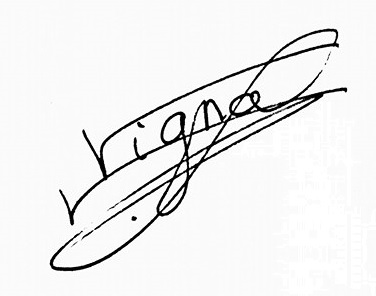
\includegraphics[scale=0.5]{images/Signature2.jpg}
    \end{figure}
    \begin{tabular}{c}
 \hrulefill \\
 Valentin Vignal \\
 \mydate\today\\
\end{tabular}
\end{center}
\newpage

% ####################################################################################################
% ####################################################################################################
% Acknowledgements
% ####################################################################################################
% ####################################################################################################

\begin{center}
    \textbf{\Large ACKNOWLEDGEMENTS}\\
\end{center}

I would like to express my special thanks and gratitude to my supervisor Harold Soh who gave me the opportunity to work on this project combining Artificial Intelligence and Music.

Secondly I would also like to thank all the members of the research team, and especially the PhD. students Abdul Fatir and Yaqi Xie who, despite their busy schedules, taught me, and help me in many scenarios.

I also would like to thank the Doctor Dorien Herremans who gave me precious advises at the beginning of my project.

\newpage
\tableofcontents
\newpage

% ####################################################################################################
% ####################################################################################################
% Summary
% ####################################################################################################
% ####################################################################################################

\setlength{\parindent}{0.6cm}

% ----- Specification -----
% The thesis must contain a summary of not more than 500 words written in the English Language. If prior approval from the Faculty has been obtained at the time of admission for a thesis to be written in a language other than English, it must contain a summary of not more than 500 words written in that language in addition to a summary not exceeding 500 words written in the English Language. The summary must be included in the thesis.

% \begin{center}
%     \textbf{\Large SUMMARY}
% \end{center}
\chapter*{Summary}
\addcontentsline{toc}{chapter}{Summary}      % To not display number of chapter in table of content

This paper introduces the work I have done for my Dissertation.
As a musician, I like to play music, improvise and create or arrange songs.

However, most of the related works about music generation with a deep neural network aim to perform one and only one task.
The main goal of this Dissertation is to create a neural network architecture able to handle several tasks a musician or a composer could perform with only one trained model.
These tasks are, completing or generating one or several musical parts, creating an accompaniment from a melody, creating a melody from an accompaniment, creating one or several musical parts from one or several other musical parts.

To this purpose, I created a new architecture that I call \textbf{RMVAE} (Recurrent Multimodal Variational AutoEncoder) which combines the MVAE architecture \cite{wu_multimodal_2018} and LSTM cells.
Only one trained model can be used to create a melody, or several musical parts at the same time, harmonize a melody or reconstruct missing parts in a song.

As a musician, I have some knowledge about musical rules and tendencies.
Therefore, I tried to incorporate some prior knowledge to the neural network with some additional custom loss functions.
I came up with 3 different functions that I named \textit{Scale}, \textit{Rhythm} and \textit{Harmony}.

For this project, I used a MIDI dataset which is Bach's Chorales dataset from the music21 corpus \cite{noauthor_music21corpuschorales_nodate} and used their framework \cite{noauthor_music21_nodate} to open and create MIDI files.
The deep learning framework I used is Tensorflow/Keras \cite{noauthor_tensorflow_nodate, noauthor_keras_nodate}.
I made my python code for this dissertation available online: \url{https://github.com/ValentinVignal/midiGenerator}.

I constructed the \textbf{RMVAE} architecture in a way that, it is easy to implement a script to handle different tasks.
The tasks I have implemented are, generate several musical parts, complete several musical parts, create a musical part from other musical parts, and re-write a song by replacing one by one all the musical parts.
Other tasks can easily be derived from the one I have already implemented.

Unfortunately, the created samples from the \textbf{RMVAE} don't match my expectations.
The model is consistent through its generation, but the quality of the created samples is poor.
The created notes are mostly Quarter notes (\musQuarter).
The model tends to generated only around 3 different notes per voice and repeat a simple sequence over and over.

I conducted some experiments and created some google forms to evaluate whether the additional loss functions actually help the model or not.
Much to my disappointment, the results of these experiments and polls weren't in favour of my custom losses.
Indeed, the results with a custom loss function are either equivalent or worse than without.


% ####################################################################################################
% ####################################################################################################
% List of Tables
% ####################################################################################################
% ####################################################################################################

\listoftables

% ####################################################################################################
% ####################################################################################################
% List of Figures
% ####################################################################################################
% ####################################################################################################

\listoffigures

% ####################################################################################################
% ####################################################################################################
% List of Illustration
% ####################################################################################################
% ####################################################################################################


% ####################################################################################################
% ####################################################################################################
% List of Syhmbols
% #####################################################################################################
% #####################################################################################################
\newpage
\begin{center}
    \textbf{\Large LIST OF SYMBOLS}\\
    \vspace{2cm}
    \begin{longtable}{ll}
        AE & Auto Encoder \\
        AI & Artificial Intelligence \\
        AMAE & ArgMax AutoEncoder \\
        C-RBM & Convolutional Restricted Boltzmann Machine \\
        CNN & Convolutional Neural Network \\
        EDM & Electronic Dance Music \\
        ELBO & Evidence Lower BOund \\
        EQL & EQuation Learner \\
        FC & Fully Connected \\
        GAN & Generative Adversarial Network \\
        GP & Gaussian Process \\
        GPU & Graphic Processing Unit \\
        GRU & Gated Recurrent Unit \\
        KLD & Kullback-Leibler Divergence \\
        LSTM & Long Short-Term Memory \\
        MCMC & Markov Chain Monte Carlo \\
        MDMM & Multimodal Deep Markov Model \\
        MiB & MebiByte \\
        MIDI & Musical Instrument Digital Interface \\
        ML & Machine Learning \\
        MVAE & Multimodal Variational AutoEncoder \\
        NADE & Neural Autoregressive Distribution Estimation \\
        NN & Neural Network \\
        PoE & Product of Experts \\
        RBM & Restricted Bolzmann Machine \\
        ReLU & Rectified Linear Unit \\
        RL & Reinforcement Learning \\
        RMVAE & Recurrent Multimodal Variational AutoEncoder \\
        RNN & Recurrent Neural Network \\
        RPoE & Recurrent Product of Experts \\
        RTRBM & Recurrent Temporal Restricted Boltzmann Machine \\
        SGD & Stochastic Gradient Descent \\
        VAE & Variational AutoEncoder \\
        VQ-VAE & Vectore Quantisation - Variational AutoEncoder \\
        VRAE & Variational Recurrent AutoEncoder \\
        VST & Virtual Studio Technology
    \end{longtable}
    
\end{center}
\newpage

\pagenumbering{arabic}

% ####################################################################################################
% ####################################################################################################
% Main body of the thesis
% #####################################################################################################
% #####################################################################################################


% ----------------------------------------------------------------------------------------------------
% Introduction
% ----------------------------------------------------------------------------------------------------
\chapter{Introduction}

As a musician, I like to play music alone or within a band.
I spend some time to create songs and arrange them. And finally, I enjoy jamming with a band and improvise.

On the deep learning part, music generation has recently considerably improved.
Models like DeepBach \cite{hadjeres_deepbach:_2016}, BachBot \cite{liang_automatic_2017}, BachDoodle \cite{huang_bach_2019} can generate, harmonized music in Bach's style.
Other non-musical model came up recently.
New architectures are being created and are able to generalize data in a more meaningful way, be more consistent through time \cite{vaswani_attention_2017}, and handle more complex data with several modalities \cite{wu_multimodal_2018-1, tan_factorized_2019}.

Therefore, I try in this work to combine my understanding of music, the knowledge so far on music generation and the capability to handle complex data with several modalities.
My goal is to create a unique model able to execute as many tasks as I could perform as a musician, which means create a song, harmonize a melody, arrange a music or jam with someone...

While I was spending my time learning about music, training my musical skills or playing with other people, I have learnt, understood and integrated some musical concepts.
Instead of letting the model learn everything from scratch from the data, I also want to give it some prior knowledge about music.

Thus, the first objective of my Dissertation is to create a unique trained model able to generate or complete a melody, generate or complete several musical parts, create an accompaniment from a melody, create a melody from an accompaniment...
The second objective is to insert some prior knowledge about music to the model.

The choices I have made for this project were mostly relying on my musical instinct.
I tried to stay as close as possible to my musical thoughts in the way I constructed a model, process the data and so on.

The chapter \ref{chap:background} will introduce to the reader some background knowledge about music and deep learning.
The chapter \ref{chap:related-works} will summarize what has already been done about music generation in deep learning, including how the data are represented, what are the objectives of these different works, what architecture they chose, and what is the generation process used.
The chapter \ref{chap:contribution} will present what are my contributions and what novel ideas I had for my Dissertation.
This will include the architecture I created (RMVAE) and how I created 3 additional loss functions to give some prior knowledge to the model.
Finally the chapters \ref{chap:results} and \ref{chap:experiments} will enumerate the results I got and what experiments I managed to conduct.


% ----------------------------------------------------------------------------------------------------
% Background
% ----------------------------------------------------------------------------------------------------
\chapter{Background}
\label{chap:background}

In this chapter, I will introduce some background knowledge that might be useful to the reader. Since this project is about music generation, I will explain and illustrate some basic concepts about music.

I will consider the Western music using equal temperament and don't consider the inharmonicity of stringed instruments. These are common assumptions in all the existing works about music generation.

The section \ref{sec:back:musical-representation} will explain how music is represented by musicians and computers and how it is possible to use those representations to create tensors.
The sections \ref{sec:back:music-theory} and \ref{sec:back:music-arrangement} will introduce the reader to basic musical rules, phenomena and definitions.
Finally, the section \ref{sec:back:nn-architectures} will enumerate several neural network architectures which are useful to understand my Dissertation.

% -------------------- Music Representation --------------------

\section{Music representation}
\label{sec:back:musical-representation}

In this section I will explain how musicians represent music on paper, and from it, how it is possible to represent music in a abstract way in a computer without encoding any waveforms or actual \textit{sounds}.

\subsection{Musical stave}

It is very useful for anyone to be able to write down their work to save it or share it with someone else. Musicians faced this issue too. They came up with the musical stave (figure \ref{fig:musical_stave_example}).

\begin{figure}[H]
    \centering
    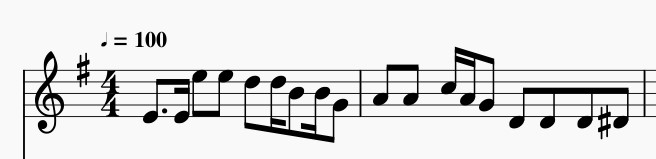
\includegraphics[scale=0.75]{images/music/stave/musical_stave_example.jpg}
    \caption{Musical Stave example}
    \label{fig:musical_stave_example}
\end{figure}

The vertical axis is the frequency axis an the horizontal axis corresponds to the time axis.
In the figure \ref{fig:musical_stave_example}, it is written that the tempo is $100 bpm$, the scale is \textit{G major} (one \musSharp) and the measure are divided with 4 beats ($4/4$ inscription).
As said previously, the vertical position of a note indicates its frequency.

\begin{figure}[H]
   \begin{minipage}{0.5\textwidth}
     \centering
     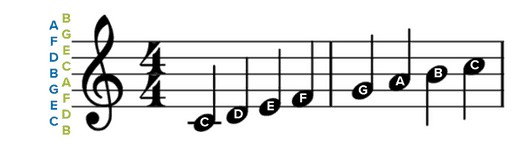
\includegraphics[width=.9\linewidth]{images/music/stave/note_names.jpg}
     \caption{Notes on a musical stave}
     \label{fig:note_names}
   \end{minipage}\hfill
   \begin{minipage}{0.5\textwidth}
     \centering
     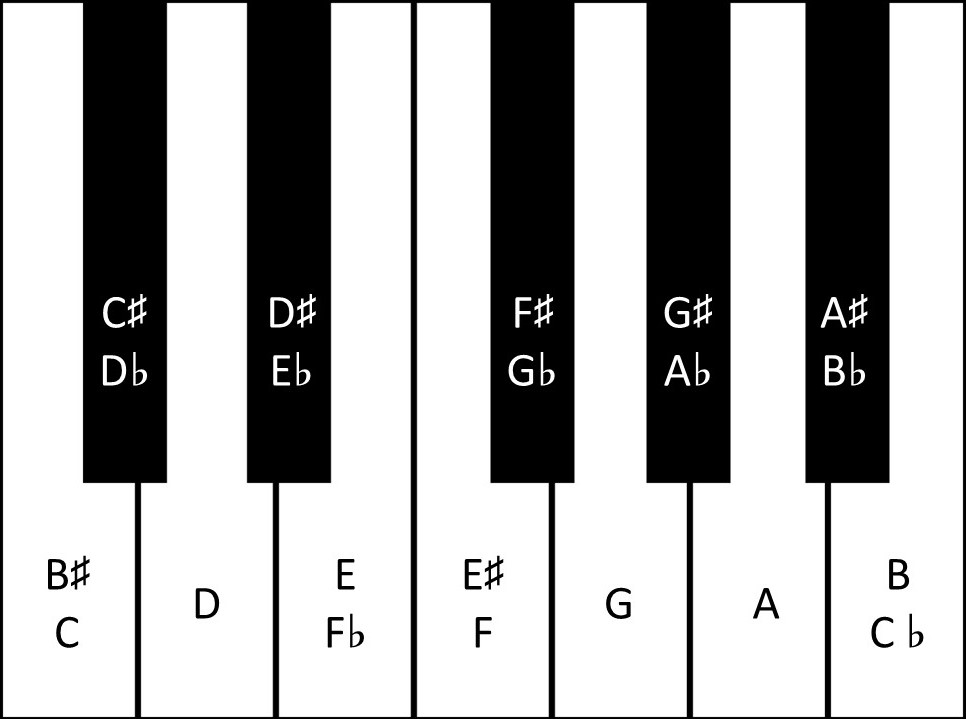
\includegraphics[width=.9\linewidth]{images/music/piano/piano_keys.jpg}
     \caption{Notes on Piano}
     \label{fig:piano_keys}
   \end{minipage}
\end{figure}

The figures \ref{fig:note_names} and \ref{fig:piano_keys} show the correspondence between the notes on a musical stave and on a piano keyboard.
By default the notes correspond to the white keys of the piano (it is the C major scale).

One thing to know is that, between 2 followings notes (or piano keys, including white and black keys), the ratio between the fundamental frequencies of the 2 notes is always equal to $\sqrt{12}$.
It means that if we consider the notes $A4$ and $A5$ (2 $A$ notes in the octaves 4 and 5), the ratio between the fundamental frequencies is $2$.
This information will help to understand chords construction.

The length of a note is defined by its shape as shown in the table \ref{tab:notes_duration}.
This table describes the relation between the length of a note, and its shape on the musical stave.

\begin{table} [ht]
    \begin{center}
        \begin{tabular} {c|c|c}
            Name & Duration & Symbol \\
            \hline
            Whole note & $4$ beats & {\Large \musWhole} \\ 
            Half note & $2$ beats & {\Large \musHalf} \\
            Quarter note & $1$ beat & {\Large \musQuarter} \\
            Eighth note & $1/2$ beat & {\Large \musEighth} \\
            Sixteenth note & $1/4$ beat & {\Large \musSixteenth} \\
        \end{tabular}
        \caption{Note names and durations}
        \label{tab:notes_duration}
    \end{center}
\end{table}

In this work, I won't consider shorter notes than Sixteenth notes because most of the songs are not using them. This is a common assumption in the existing works.


\subsection{MIDI}
\label{sec:midi}

% The \textit{MIDI} format ($.mid$) is a format to save music as a file. However, it doesn't save the actual \textit{sound} of it. The way it works is very similar to the representation of a musical stave.

% In a midi file is a set of instructions. It will save for each instruments, for each notes (pitch) the times when the note starts and ends and some other information (like the velocity et caetera).

% To read a midi file, the computer has a collection of sound for every instruments, notes, velocity et caetera, and plays these sounds depending of the instructions read in the file.

The \textit{MIDI} format ($.mid$) is a technical standard that describes a protocol.
It was first used to carry musical messages between electronic instruments, software and any musical devices.
These messages are musical events. It contains note information as the pitch, the velocity, or the panning, and some other parameters (for example, vibrato, volume...). 
The most important messages I will consider are:
\begin{itemize}
    \item \textit{Note on} which indicates that a note has to be played. It contains the channel information (which can be considered as an instrument), the pitch information (what note should be played) and the velocity. We could right an event as follow :
    \begin{equation}
        <NoteOn, 0, 50, 127>
    \end{equation}
    to describe the event \textit{"Start to play the note $D3$ (50) with the maximum velocity (127) for the channel (instrument) 0"}.
    \item \textit{Note off} which indicates to stop playing a note (for instance, release the keyboard key). The given parameters are the same as the ones given to the \textit{Note On} event.
    \begin{equation}
        <NoteOff, 0, 50, 127>
    \end{equation}
    will stop the note started with the previous \textit{Note On} event.
\end{itemize}

Each note is associated with a time value.
It can be expressed in number of ticks (time division). The header of file specifies how may ticks there are per quarter note.

\subsection{Pianoroll}

The pianoroll is a common representation of a musical stale in music production softwares.

\begin{figure}[H]
    \centering
    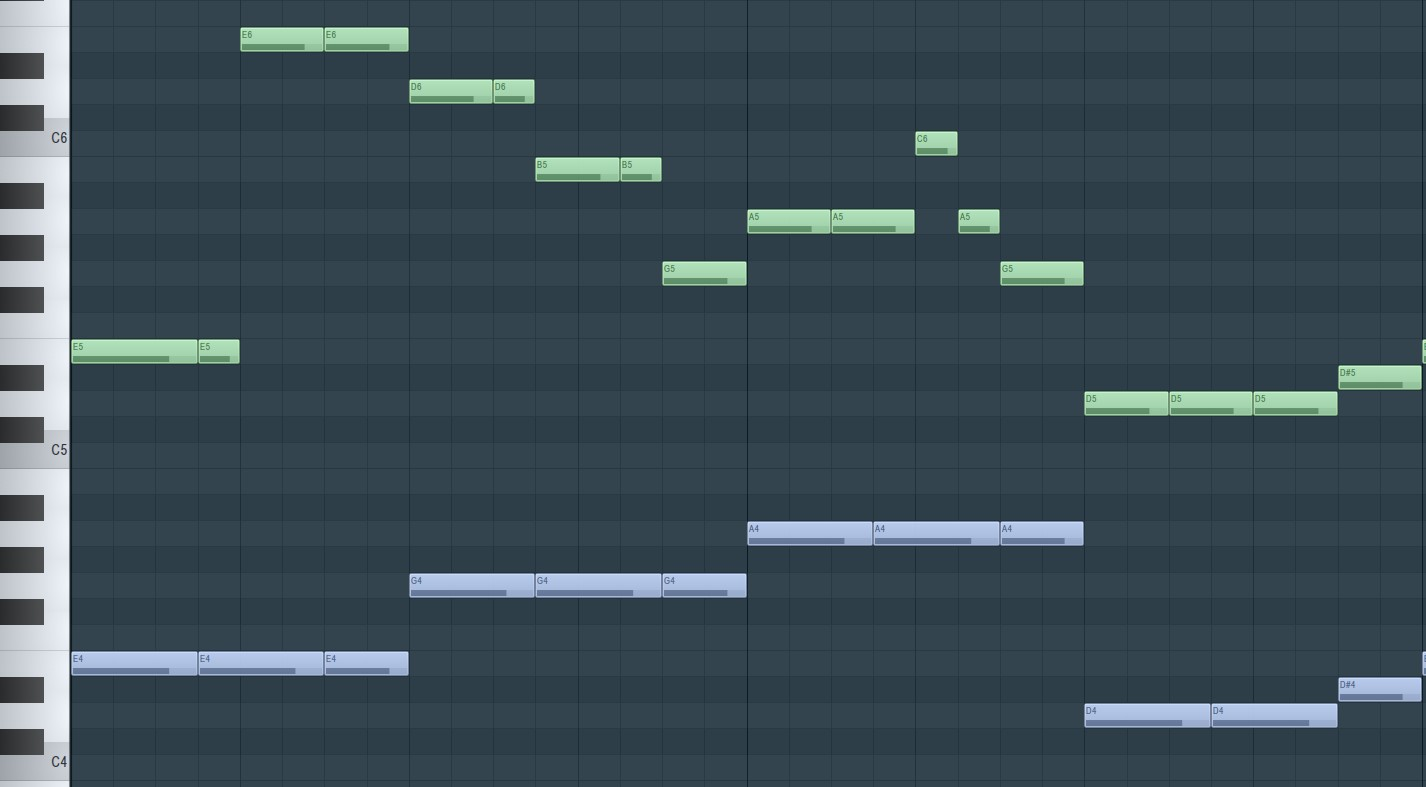
\includegraphics[width=0.75 \textwidth]{images/music/pianoroll/pianoroll_flstudio.jpg}
    \caption{Pianoroll example from the software FL Studio \cite{noauthor_fl_nodate}}
    \label{fig:pianoroll_flstudio}
\end{figure}

The figure \ref{fig:pianoroll_flstudio} shows a view of the pianoroll in the famous software \textit{FL Studio} \cite{noauthor_fl_nodate}. The composers of electronic music like EDM, Techno and so on use this view to compose and arrange their songs.

% -------------------- Music Theory --------------------

\section{Music theory}
\label{sec:back:music-theory}

In this section, I will describe and explain some rules from music theory which are related to this work.
The rules I am going to explain are the most common ones and most of the songs tend to follow them.

\subsection{Scale and Rhythm}

\subsubsection{Scale}

A \textit{scale} is a set of notes.
Because the human ear is now used to it, the notes of a scale will sound nice when they are played together.
In traditional Western music, it generally consists of 7 notes.
There are several types of scales.
The most common one is the \textit{Major Scale} or the \textit{Natural Minor Scale}.
For example, the C Major scale uses all the white keys of the piano (figure \ref{fig:piano_keys}: A, B, C, D, E, F and G), as well as the A Natural Minor scale.

Another type of scale, often used by the musicians to creates their \textit{solos}, is the \textit{Pentatonic} scale.


\begin{figure}[H]
    \centering
    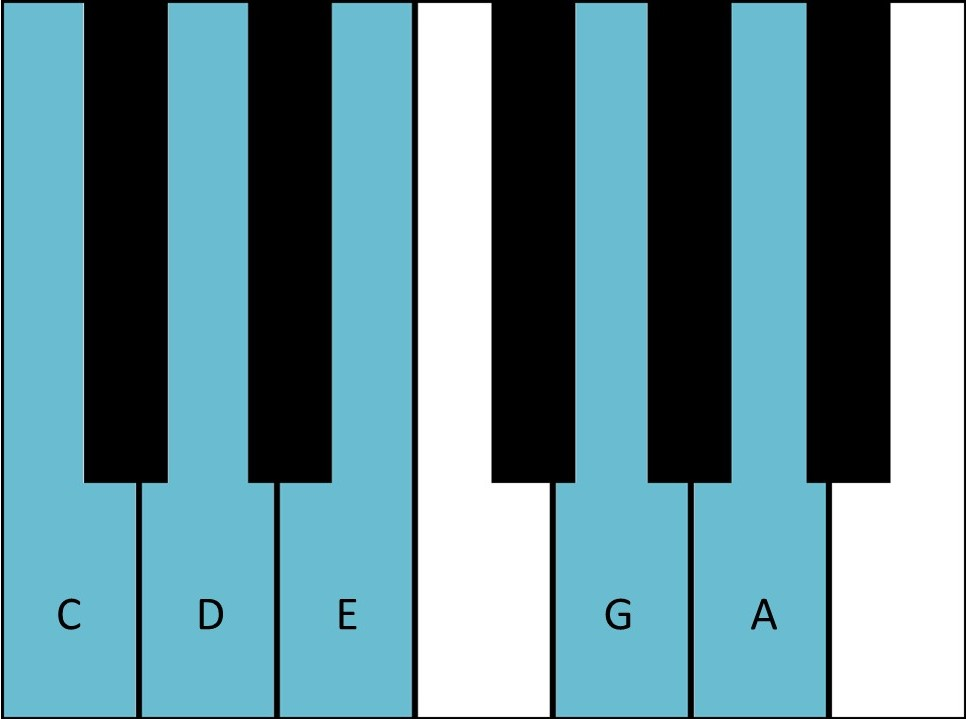
\includegraphics[width=0.5 \textwidth]{images/music/piano/pentatonic_scale.jpg}
    \caption{C Major Pentatonic scale (or A Minor Pentatonic scale)}
    \label{fig:pentatonic_scale_piano}
\end{figure}

As seen in the figure \ref{fig:pentatonic_scale_piano}, the C Major pentatonic scale (which uses the same notes as the A Minor pentatonic scale) uses only five notes (A, C, D, E and G) which are contained in the C Major Scale.
It is known that playing in this scale will easily produce enjoyable and in-tune melodies or any musical parts.


\subsubsection{Rhythm}

The rhythm is an important part of current music like \textit{Pop Music}.
It has the tendency to remain consistent through the song and repeat some patterns.
It helps the listener to easily follow the progression and allows him to listen what he's expecting to.

However, rhythm is more flexible than scale and harmonies, and there is no rhythm theory someone could follow.
This is why classical music is not considered as a rhythmic music.

I this work, I considered and will consider only binary rhythm (each beat is divided into 2 smaller equal beats) and not ternary rhythm (each beat is divided into 3 smaller equal beats) because the binary rhythm is the most common one.


\subsection{Harmonics}
\label{sec:harmonics}

In this section, I will introduce some physical concept about musical sounds and timbres and then illustrate how it can explain some musical rules.

\subsubsection{Harmonics}

A sound is a sum of harmonics (equation \ref{eq:harmonics}).

\begin{equation}
    s(t) = \sum_{n=1}^{\infty} \alpha_{n} \sin(n f t + \phi_{n})
    \label{eq:harmonics}
\end{equation}
where $f$ is the fundamental frequency and $\phi$ the phase.

Let us take an example with the $A4$ note which has its fundamental frequency equals to $440 Hz$.
The $2^{nd}$ harmonic is $A5$ $880Hz$.
The consequence is, when an instrument plays a $A4$, all the harmonics of a $A5$ are also present.
Let us take one step further, the $3^{rd}$ harmonic of $A4$ is $E5$ $1320Hz$.
It means it is possible to hear a $E5$ from a played $A4$.
The table \ref{tab:A4_harmonics} references the first harmonics of the $A4$ note.

\begin{table} [ht]
    \begin{center}
        \begin{tabular} {c||c|c|c}
            Harmonic number & Frequency ($Hz$) & Note Name & Musical Interval \\
            \hline
            $1$ & $440$ & $A4$ & Unison \\
            $2$ & $880$ & $A5$ & Octave \\
            $3$ & $1320$ & $E5$ & Fifth \\
            $4$ & $1760$ & $A6$ & Octave \\
            $5$ & $2200$ & $C\sh6$ & Major Third \\
            $6$ & $2640$ & $E6$ & Fifth \\
        \end{tabular}
        \caption{Harmonics of $A4$}
        \label{tab:A4_harmonics}
    \end{center}
\end{table}

From the table \ref{tab:A4_harmonics}, we can notice:
\begin{itemize}
    \item The $A$ and $E$ notes are linked together (\textit{Fifth} or reversed \textit{Fourth} interval).
    \item The $A$ and $C\sh$ notes are linked together (\textit{Major Third} interval).
\end{itemize}


\subsubsection{Chords}

The links between notes illustrated in the table \ref{tab:A4_harmonics} explain why a Major chord sounds \textit{nice} or \textit{smooth}.
A $A$ $Major$ chord is composed with 3 notes : $A$, $C\sh$ and $E$. All the notes are already contained in the harmonics of a $A$ sound.

A Minor chords ($A$ $Minor$ is $A$, $C$, $E$) will also sounds acceptable to the human ears because $A$ and $C$ share $E$ in their harmonics (respectively the \textit{Fifth} interval and \textit{Third Major} interval) 

\subsubsection{Dissonance}

When 2 frequencies are close to each other and added up, a resonance phenomena is observed.

\begin{figure}[H]
    \centering
    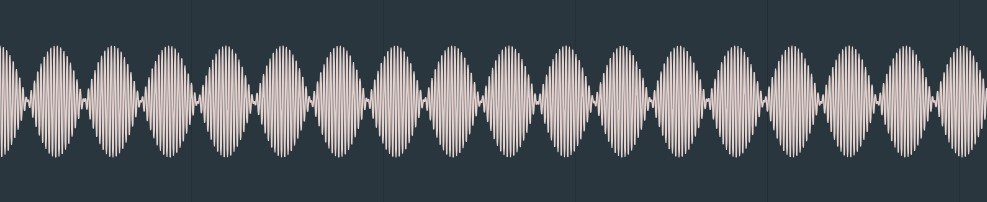
\includegraphics[width=\textwidth]{images/music/waveform/resonance.jpg}
    \caption{Resonance waveform}
    \label{fig:resonance}
\end{figure}
The figure \ref{fig:resonance} shows the waveform generated by a $B4$ ($494Hz$) and a $C5$ ($523Hz$) (\textit{semitone} interval).
This resonance is explained by the trigonometric identity written in the equation \ref{eq:resonance}.

\begin{equation}
    \cos(f) + \cos(f + \delta f) = 2 \cos(\frac{2f + \delta f}{2}) \cos(\frac{\delta f}{2})
    \label{eq:resonance}
\end{equation}

This phenomena is unpleasant to hear and this is why, musicians usually avoid to play notes that generate a resonance with their harmonics:
\begin{itemize}
    \item \textit{Semitone} interval (ex: $A$ and $A\sh$)
    \item \textit{Tone} interval (ex: $A$ and $B$)
    \item \textit{Tritone} interval (ex: $A$ and $D\sh$)
\end{itemize}


\subsubsection{Harmony}

Either for classical music (Bach Chorales) or pop music (back singers), a common method to \textit{fill a song} is to add harmony parts to the lead melody. The harmony parts usually follow the lead melody but on other notes.
An example is provided in the figure \ref{fig:harmony_example}.

\begin{figure}[H]
    \centering
    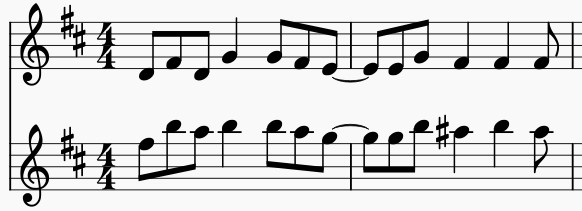
\includegraphics[width=0.75 \textwidth]{images/music/stave/harmony.jpg}
    \caption{Lead voice and its harmony part}
    \label{fig:harmony_example}
\end{figure}

The harmony parts will usually avoid unpleasant interval and mostly try to create the following ones: 
\begin{itemize}
    \item \textit{Octave} and \textit{Unison} interval
    \item \textit{Fifth} interval
    \item \textit{Fourth} interval
    \item \textit{Major Third} interval
    \item \textit{Minor Third} interval
\end{itemize}


% -------------------- Music arrangement  --------------------

\section{Music arrangement}
\label{sec:back:music-arrangement}

Arranging a song is an entire musical field an a job.
It is the art of giving to an existing melody musical variety.
To put it more simply, it means creating a accompaniment from a melody.
To do so, the musician can include chords, change the rhythm, add other musical parts...

To give an example, arranging a song could be creating piano, guitar, drums and bass parts from a voice melody with lyrics.


% -------------------- Neural Network architecture --------------------

\section{Neural Network architectures}
\label{sec:back:nn-architectures}

In this section, I will briefly describe some neural network architectures.

\subsection{Convolutional neural network}

Convolutional neural networks are often used on images because of their ability to preserve the spatial information.
A CNN usually includes two types of layers:
\begin{itemize}
    \item A convolutional layer
    \item A pooling layer
\end{itemize}

\subsubsection{Convolutional Layer}

For a 2D convolution, a convolutional layer takes as an input a tensor of shape \texttt{(height, width, channels)}.
The \textit{filter} of the convolutional layer will have a shape \texttt{(h, w, channels)}.
Then the layer will do a $2D$ convolutional operation between the filter and the input through the axes corresponding to the \texttt{height} and the \texttt{width}.

\begin{equation}
    y_{\tau} = \sum_{t=0}^{l-1} w_{t} \times x_{\tau + t}
    \label{eq:convo}
\end{equation}

The equation \ref{eq:convo} shows the mathematical transformation for a 1D convolution with $x$ as the input, $w$ as the filter/kernel and $y$ as the output.

\subsubsection{Pooling Layer}

A pooling layer is used to reduce the size of a tensor. It extracts a value from a region of the tensor. Two common pooling operations are:
\begin{itemize}
    \item The \textit{Average pooling} which takes the average of the region
    \item The \textit{Max pooling} which takes the maximum of the region
\end{itemize}
The figure \ref{fig:max_pooling} illustrates how the max pooling operation works.

\begin{figure}[H]
    \centering
    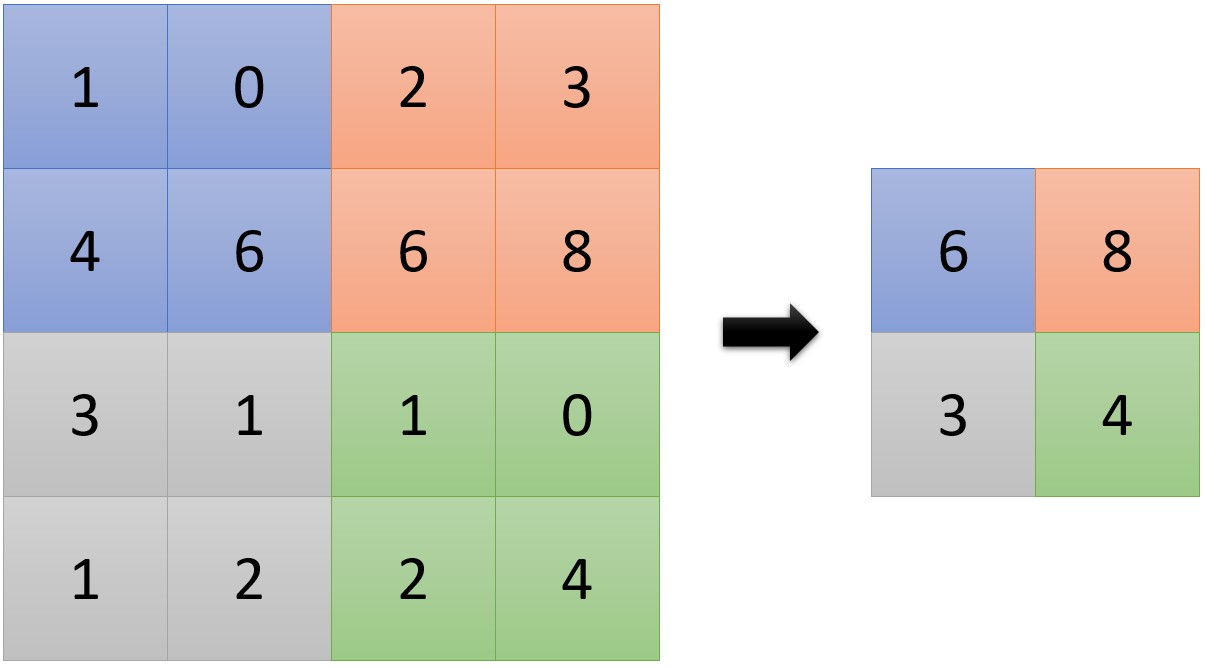
\includegraphics[width=0.75 \textwidth]{images/nn/layers/max_pooling.jpg}
    \caption{Max pooling operation}
    \label{fig:max_pooling}
\end{figure}

\subsection{AutoEncoder}
\label{sec:back:ae}

An AE \cite{moor_topological_2020, tschannen_recent_2018, rudolph_structuring_2019} is composed of a \textit{encoder} and a \textit{decoder}.
First, the input goes into the encoder.
The output of the encoder is the latent space (the hidden layer), which is smaller than the input.
The output of the encoder becomes the input of the decoder.
The goal of the decoder is to reconstruct the input from the latent space.
The hidden layers of the AE are smaller than the input.
It forces the network to compress the input and reduce its dimensions.
Therefore, the AE has to learn "high level features" about the inputs.
The figure \ref{fig:autoencoder} summarizes this architecture.

\begin{figure}[H]
    \centering
    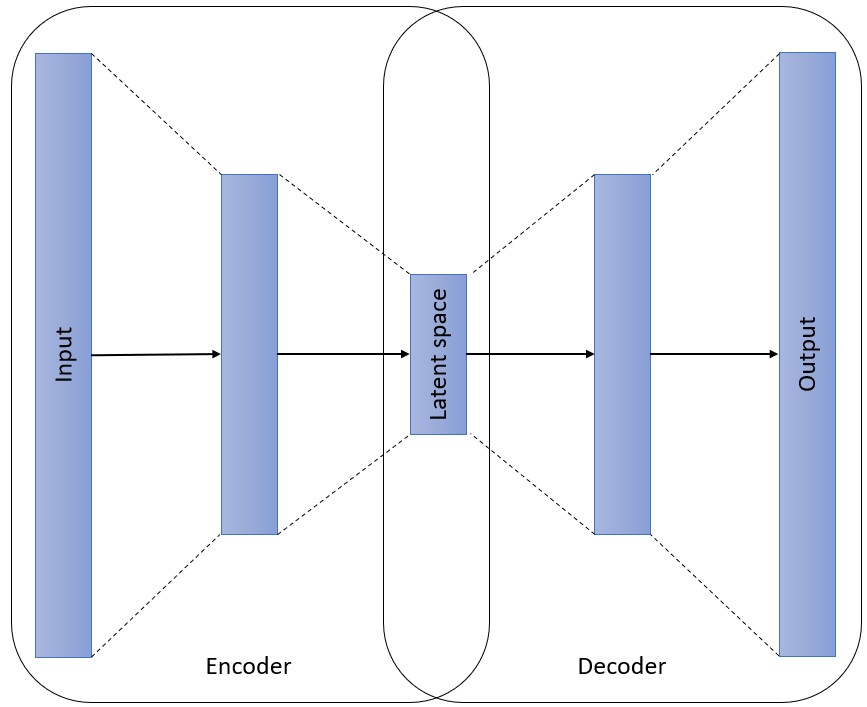
\includegraphics[width=0.9 \textwidth]{images/nn/architectures/autoencoder.jpg}
    \caption{AutoEncoder}
    Source: \href{https://commons.wikimedia.org/wiki/File:Autoencoder_structure.png}{Wikipedia}
    \label{fig:autoencoder}
\end{figure}

\subsection{Variational AutoEncoder}
\label{sec:back:vae}

The VAE \cite{doersch_tutorial_2016, noauthor_variational_nodate, noauthor_tutorial_nodate, akrami_robust_2019, liu_towards_2020} comes from the Bayesian Theorem (equation \ref{eq:bayesian-theorem}).

\begin{equation}
    p(x|z) = \frac{p(z|x) p(x)}{p(z)}
    \label{eq:bayesian-theorem}
\end{equation}

It is a latent variable generative model of the form $p_{\theta}(x, z) = p(z)p_{\theta}(x|z)$ where $p(z)$ is the prior.
$z$ is usually a standard Gaussian distribution: $z \sim \mathcal{N} (0, I)$.
The decoder $p_{\theta}(x|z)$ is a neural network, with the parameters $\theta$ composed with a simple likelihood (for example, a Bernoulli or Gaussian distribution).
The training's objective is to maximize the marginal likelihood of the data (called the \textit{"evidence"}) (equation \ref{eq:vae:argmax}).
\begin{equation}
    \text{argmax}_{\theta} (\log(p_{\theta} (x)))
    \label{eq:vae:argmax}
\end{equation}
However, since it is intractable (equation \ref{eq:vae:intractable}), the evidence lower bound is instead optimized. The ELBO is defined via a neural network $q_{\phi}(z|x)$, with parameters $\phi$ which serves as a intractable importance distribution (equation \ref{eq:vae:elbo}).
\begin{equation}
    \log (p_{\theta} (x)) = \log \left( \int_{z} p_{\theta} (x|z) p(z) dz\right)
    \label{eq:vae:intractable}
\end{equation}
\begin{equation}
    \text{ELBO}(x) = \mathbb{E}_{q_{\phi}(z|x)} \left[ \log (p_{\theta}(x|z)) \right] - \mathbb{D}_{KL} \left( q_{\phi}(z|x), p(z) \right)
    \label{eq:vae:elbo}
\end{equation}
Where $\mathbb{D}_{KL}(p, q)$ is the Kullback-Leibler divergence between distributions $p$ and $q$.
The ELBO is usually optimized via stochastic gradient descent, using reparameterization trick to estimate the gradient \cite{kingma_auto-encoding_2014}.

The figure \ref{fig:vae:reparameterization-trick} shows the reparameterization trick.
At training-time, VAE is implemented as a feed forward neural network, where $p(x|z)$ is Gaussian.
Left is without the reparameterization trick, and right is with it.
Red shows sampling operations that are non-differentiable.
Blue shows loss layers.
The feed forward behavior of these networks is identical, but the backpropagation can be applied only to the right network.

\begin{figure}[htbp]
    \centering
    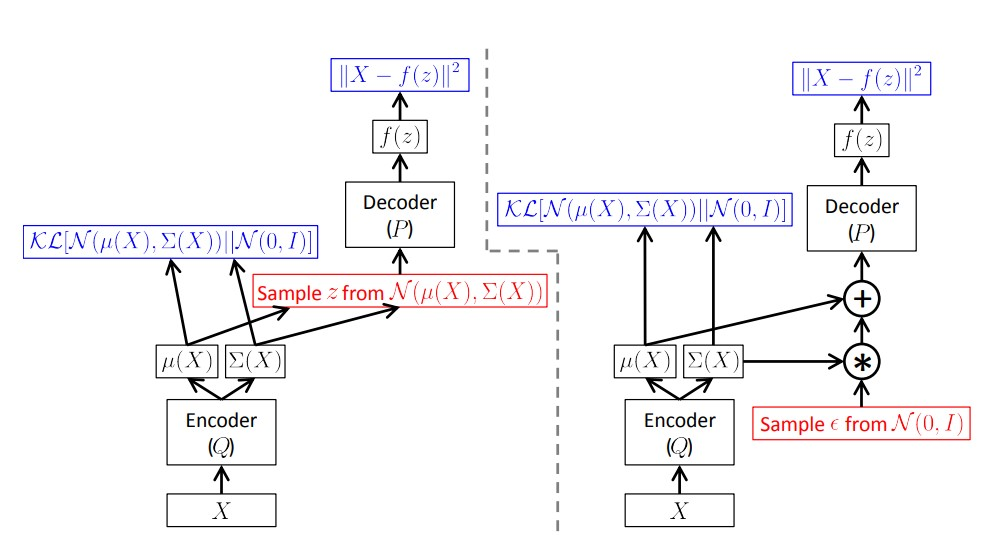
\includegraphics[width=\textwidth]{images/nn/architectures/reparameterization-trick.jpg}
    \caption{Reparameterization trick for VAE}
    Source: Tutorial on Variational Autoencoders \cite{doersch_tutorial_2016}
    \label{fig:vae:reparameterization-trick}
\end{figure}

\subsubsection{Summary and vulgarization of VAE}

A VAE  is an autoencoder. The steps are the following:
\begin{enumerate}
    \item The input goes first in the encoder which encodes it as a Gaussian distribution over the latent space.
    \item A point is sample from this distribution.
    \item This point is decoded by the decoder to reconstruct the input.
\end{enumerate}

By encoding the normal distribution and not directly the latent space, it is possible to regularize the output of the encoder to avoid overfitting and ensure that the latent space has good properties to enable generative process.

To regularize the output of the decoder, an extra term is added to the loss function : Kullback-Leibler Divergence (KLD) between the encoded distribution and the centred and reduced normal distribution :

\begin{equation}
    \mathbb{D}_{KL} (\mathcal{N}(\mu_{encoded}, \sigma_{encoded}), \mathcal{N}(0, 1))
\end{equation}

\subsection{Generative Adversarial Network}
\label{sec:back:gan}

The idea of GANs \cite{noauthor_gan_2017, goodfellow_generative_2016, goodfellow_generative_2014, goodfellow_nips_2017} is to set up a game between two players.
The first player is called the \textit{generator} and creates samples.
These samples are intended to come from the same distribution as the training data.
The second player is called the \textit{discriminator}.
He examines samples to determine whether they are real or fake.
The discriminator learns using traditional supervised learning techniques, dividing inputs into two classes (real or fake).
The generator is trained to fool the discriminator.

GANs are a structured probabilistic model containing latent variables $z$ and observed variables $x$ (figure \ref{fig:gan-latent-space}).

\begin{figure}[htbp]
\begin{center}
    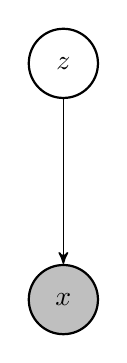
\begin{tikzpicture}[->, >=stealth', auto, semithick, node distance=3cm]
    \tikzstyle{every state}=[fill=white,draw=black,thick,text=black,scale=1]
    
    \node[state](z){$z$};
    \node[state, fill=lightgray](x)[below of=z]{$x$};
    
    \path
        (z) edge    node{}    (x);
    \end{tikzpicture}
\caption{The graphical model structure of GANs}
\label{fig:gan-latent-space}
\end{center}
\end{figure}

The two players in the game are represented by two differentiable functions.
The discriminator is a function $D$ that takes $x$ as input and uses $\theta^{(D)}$ as parameters.
The generator is defined by a function $G$ that takes $z$ as input and uses $\theta^{(G)}$ as parameters.

Both players have a cost function which depends on the parameters of both players.
The discriminator tries to minimize $J^{(D)} (\theta^{(D)}, \theta^{(G)})$ by controlling $\theta^{(D)}$.
The generator tries to minimize $J^{(G)} (\theta^{(D)}, \theta^{(G)})$ by controlling $\theta^{(G)}$.
Because each player’s cost depends on the other player’s parameters, but each player can only modify its own parameters, this scenario can be described as a game.
The solution to a game is a called a Nash equilibrium.
For us, a Nash equilibrium is a tuple $(\theta^{(D)}, \theta^{(G)})$ that is a local minimum of $J^{(D)}$ with respect to $\theta^{(D)}$ and a local minimum of $J^{(G)}$ with respect to $\theta^{(G)}$.

The generator is simply a differentiable function $G$ represented by a deep neural network.
When $z$ is sampled from some simple prior distribution, $G(z)$ yields a sample of $x$ drawn from $p_{model}$.

The figure \ref{fig:gan-framework} illustrates the framework of GANs.

\begin{figure}[htbp]
    \centering
    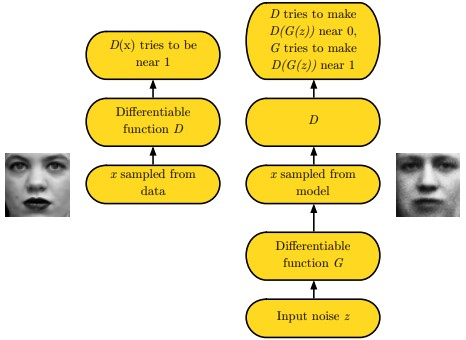
\includegraphics[width=\textwidth]{images/nn/architectures/gan-framework.jpg}
    \caption{GAN framework}
    \label{fig:gan-framework}
    Source: Ian Goodfellow's paper \cite{goodfellow_nips_2017}
\end{figure}

\subsubsection{Discriminator cost function}

The cost function used for the discriminator is showed in the equation \ref{eq:gan:cost-d}.
\begin{equation}
    J^{(D)}(\theta^{(D)}, \theta^{(G)}) = -\frac{1}{2}\mathbb{E}_{x \sim p_{data}} (\log (D(x))) - \frac{1}{2} \mathbb{E}_{z} ( \log (1 -D(G(z)))
    \label{eq:gan:cost-d}
\end{equation}

\subsubsection{Generator cost functions}

There are several possibilities for the cost function of the generator.

\paragraph{Minimax}:

The first one is the \textbf{Minimax} cost function: $J^{(G)} = - J^{(D)}$.
This a \textit{zero-sum game}.
Zero-sum games are also called \textbf{minimax} games because of the form of the solution (equation \ref{eq:gan:minimax}).
\begin{equation}
    \theta^{(G)*} = \text{argmin}_{\theta^{(G)}} \left[ \text{argmax}_{\theta^{(D)}} \left[ J^{(G)} \left( \theta^{(D)}, \theta^{(G)} \right) \right] \right]
    \label{eq:gan:minimax}
\end{equation}

\paragraph{Heuristic, non-saturating game}:

The second one is the \textbf{Heuristic, non-saturating game}.
The minimax cost function doesn't perform well in practice.
If the discriminator performs too well compared to the generator, it will successfully reject the samples from the generator with high confidence.
The gradient of the generator will then start to vanish.
In the Heuristic, non-saturating game version, the generator cost is the equation \ref{eq:gan:heuristic}
\begin{equation}
    J^{(G)} = - \frac{1}{2} \mathbb{E} (\log(D(G(z))))
    \label{eq:gan:heuristic}
\end{equation}
The motivation of this cost function is to ensure that each player has a strong gradient when it is \textit{"losing"} the game.

\paragraph{Maximum likelihood game}:

The third one is the \textbf{Maximum likelihood game}.
This version maximizes the likelihood learning with GANs.
It means it minimizes the KLD between the data and the model.
In its paper \cite{goodfellow_generative_2014}, Goodfellow showed that using the equation \ref{eq:gan:likelihood} is equivalent to minimize the KLD between the data and the model.
In the equation \ref{eq:gan:likelihood}, $\sigma$ is the logistic function.
\begin{equation}
    G^{(G)} = - \frac{1}{2} \mathbb{E}_{z} \left[ \exp \left( \sigma^{-1} (D(G(z))) \right) \right]
    \label{eq:gan:likelihood}
\end{equation}

\subsubsection{Divergence choice}

The choice of the divergence will influence the results of the training.
The KLD is not symmetric.
Minimizing $\mathbb{D}_{KL}(p_{data}, p_{model})$ is different from minimizing $\mathbb{D}_{KL}(p_{model}, p_{data})$.
The figure \ref{fig:gan:directions-kld} shows the differences between the two directions of the KLD.
\begin{figure}[htbp]
    \centering
    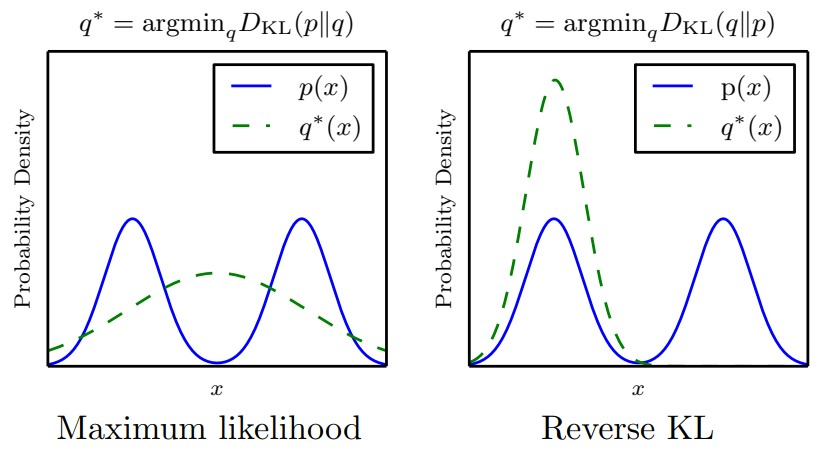
\includegraphics[width=\textwidth]{images/nn/graphs/reverse-kl.jpg}
    \caption{Differences between the two direction of the KLD}
    Source: Ian Goodfellow's paper \cite{goodfellow_nips_2017}
    \label{fig:gan:directions-kld}
\end{figure}
Minimizing the reverse KL might be expected to yield better samples because the model will generate samples that come only from modes in the training distribution.
It will ignore some modes and won't try to include all of them with the risk of generating some samples that don't belong to any training set mode.

\subsubsection{Summary and vulgarization of GANs}

GANs are composed of two models that are trained simultaneously:
\begin{itemize}
    \item The \textit{Generator} will learn how to create data that look real.
    \item The \textit{Discriminator} will learn how to differentiate real and generated data.
\end{itemize}

The discriminator is trained with real data and data generated by the generator.
The goal of the discriminator is to classify the real data as \textit{"Real"} and the generated data as \textit{"Fake"}.
On the other side, the generator takes some noise as an input to generate a datum.
Its goal is to make the discriminator classify its generated data as \textit{"Real"}.

Through training, the generator will get better and create more consistent data so the discriminator classify them as \textit{"Real"}.
It will then force the discriminator to become better and classify real and fake data more precisely.
Thus, the generator is forced to create data which look more real.
And so on...

\subsection{Recurrent Neural Networks}
\label{sec:back:rnn}

A RNN \cite{chen_gentle_2018} is a neural network where connections between nodes form a direct graph along a temporal sequence. The general architecture is showed in the figure \ref{fig:rnn}.

\begin{figure}[htbp]
    \centering
    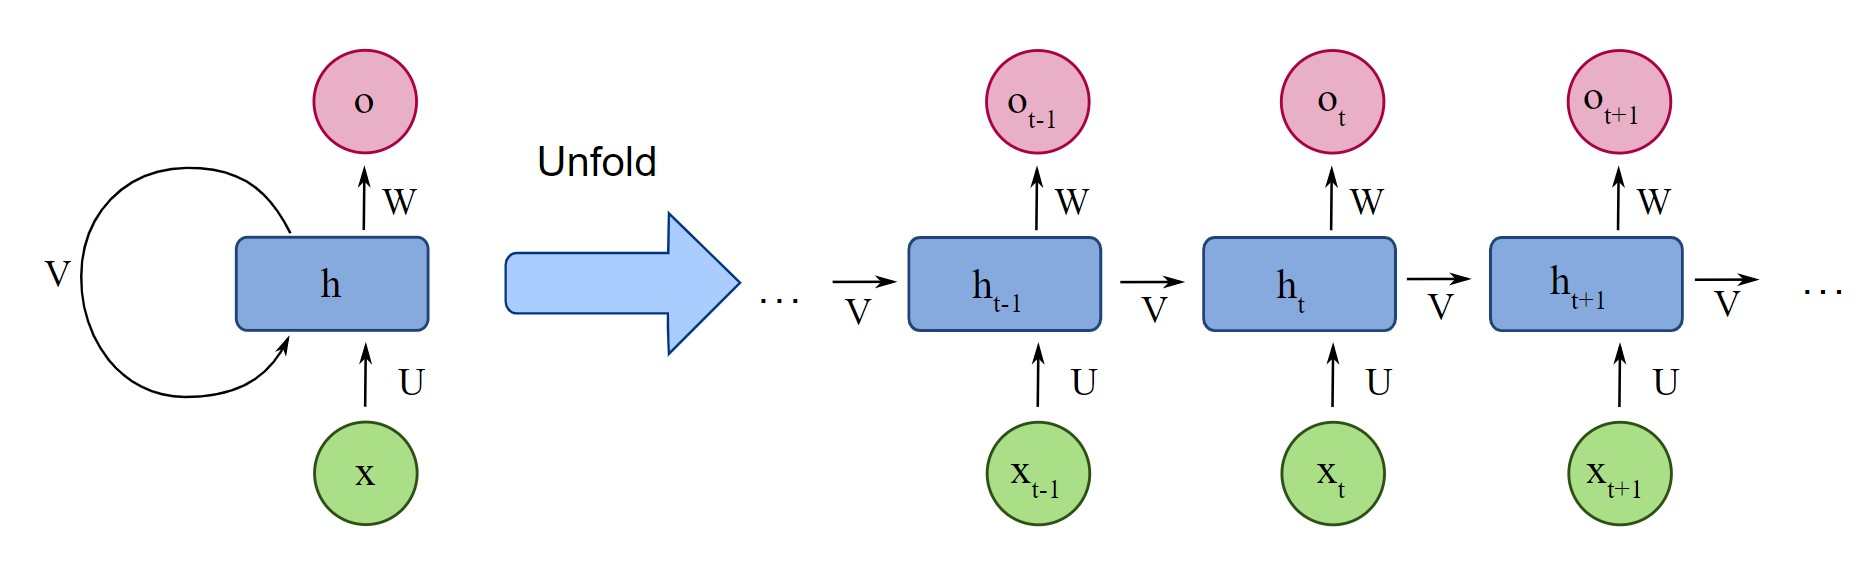
\includegraphics[width=0.9\textwidth]{images/nn/architectures/rnn.jpg}
    \caption{Recurrent Neural Network}
    Source: Gang Chen's paper \cite{chen_gentle_2018}
    \label{fig:rnn}
\end{figure}

The most used cells are the LSTM cell and the GRU cell. The architectures are showed in the figures \ref{fig:lstm-gru}.

\begin{figure}[htbp]
    \centering
    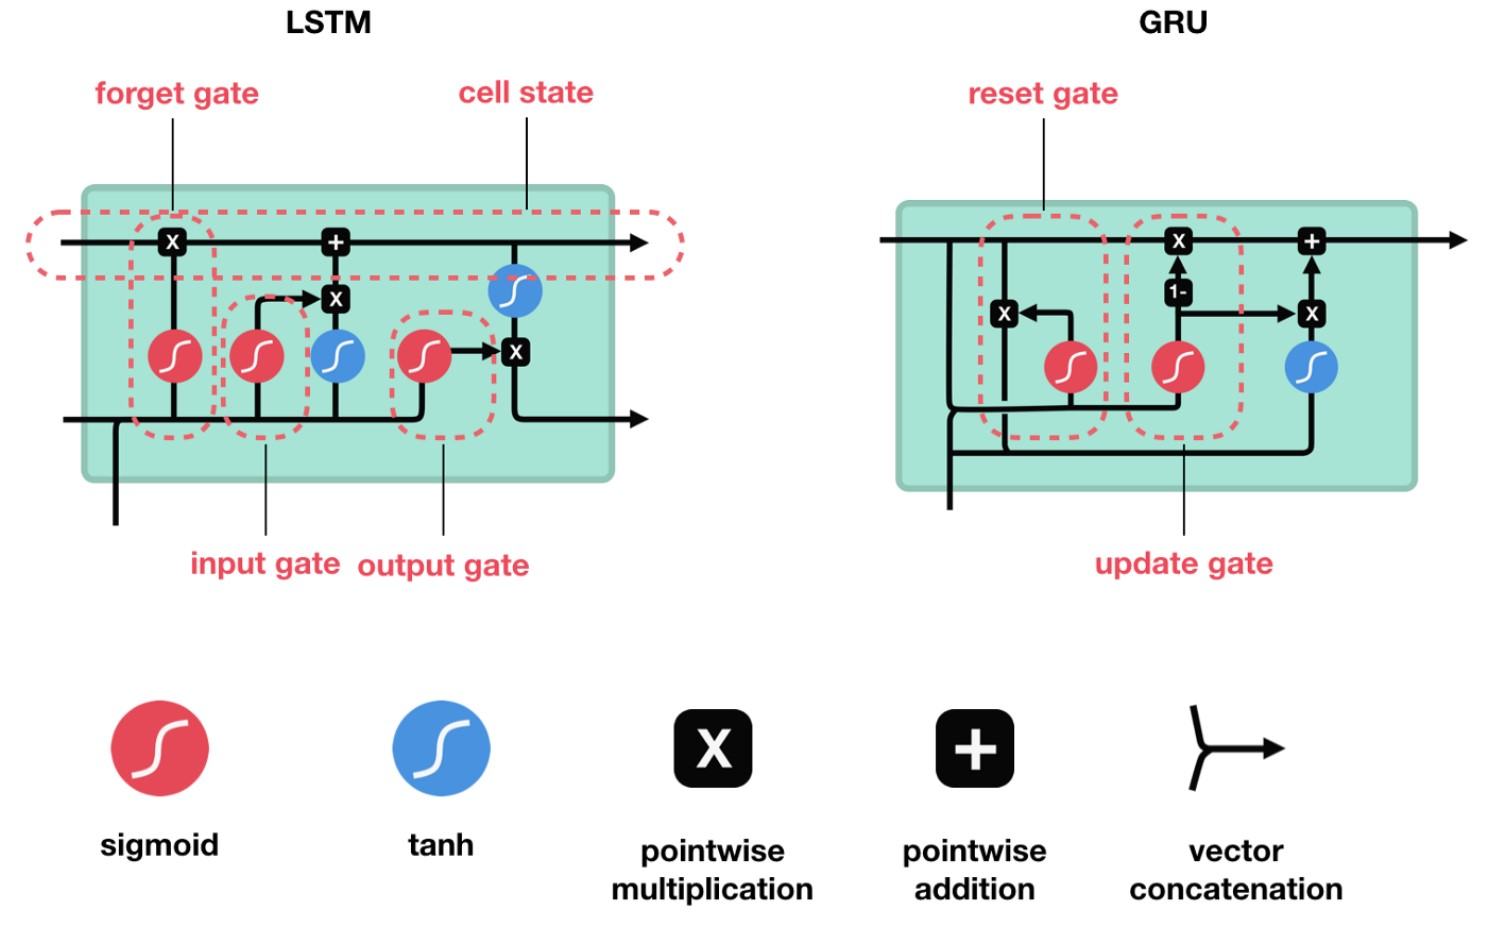
\includegraphics[width=\textwidth]{images/nn/layers/lstm-gru.jpg}
    \caption{LSTM and GRU cell}
    Source: Michael Nguyen's tutorial \cite{nguyen_illustrated_2019}
    \label{fig:lstm-gru}
\end{figure}


\subsection{Transformers}
\label{sec:back:transformers}

Transformers \cite{vaswani_attention_2017, noauthor_transformer_nodate, giacaglia_transformers_2019, allard_what_2020, alammar_illustrated_nodate} have been introduced to the world by Ashish Vaswani et al. \cite{vaswani_attention_2017-1}.
It is an attention mechanism illustrated in the figure \ref{fig:arch:transformer}.
On this figure, the encoder is on the left and the decoder on the right.

The scaled dot-product attention and multi-head attention layers are drawn in the figures \ref{fig:scaled_dot_product_attention} and \ref{fig:multi_head_attention}.

\begin{figure}[htbp]
    \centering
    \newlength{\MyOtherHeightFour}
    \settoheight{\MyOtherHeightFour}{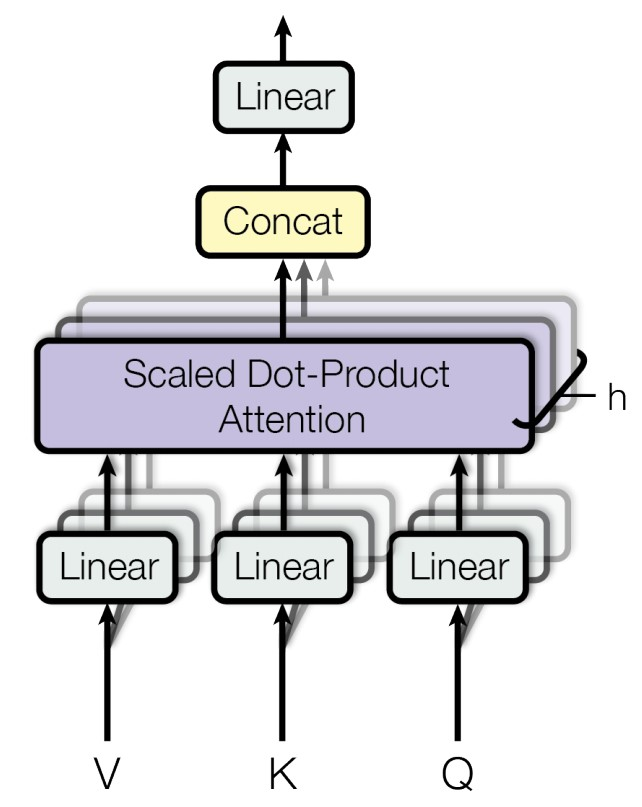
\includegraphics[width=0.9 \textwidth]{images/related_works/transformer/multi_head_attention.jpg}}
    \begin{subfigure}[t]{0.49\textwidth}
        \centering
        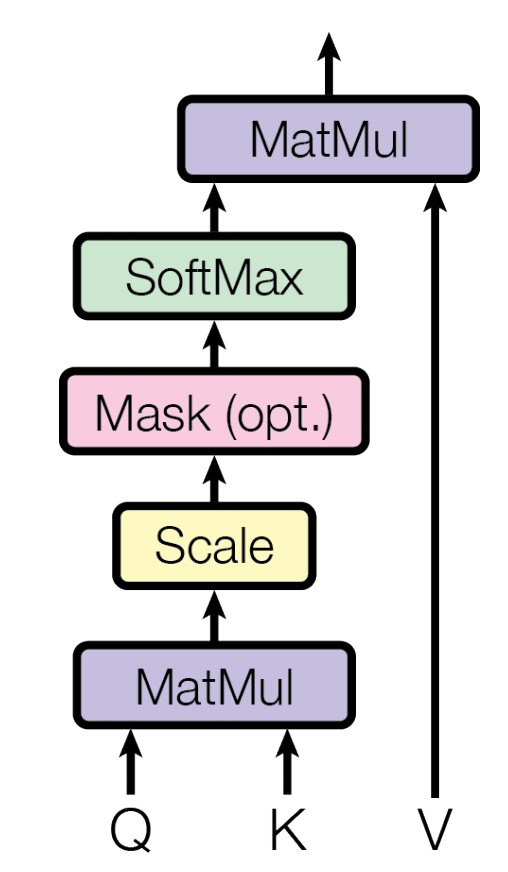
\includegraphics[width=.6\textwidth]{images/related_works/transformer/scaled_dot_product_attention.jpg}
        \caption{Scaled Dot-Product Attention}
        Source: Ashish Vaswani et al.'s paper \cite{vaswani_attention_2017-1}
        \label{fig:scaled_dot_product_attention}
    \end{subfigure}
    \hfill
    \begin{subfigure}[t]{0.49\textwidth}
        \centering
        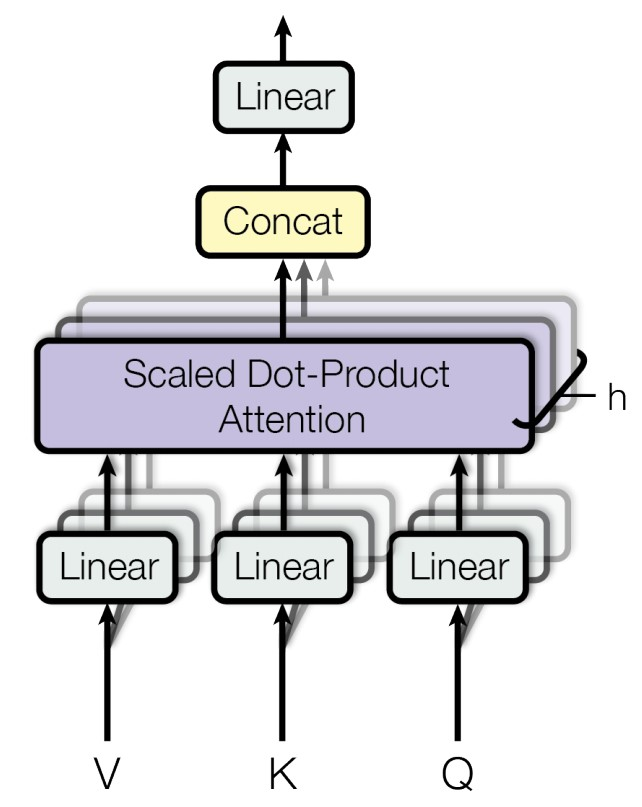
\includegraphics[width=.9 \textwidth]{images/related_works/transformer/multi_head_attention.jpg}
        \caption{Multi-Head Attention}
        Source: Ashish Vaswani et al.'s paper \cite{vaswani_attention_2017-1}
        \label{fig:multi_head_attention}
    \end{subfigure}
    \caption{Scaled Dot-Product Attention and Multi-Head Attention}
    Source: Ashish Vaswani et al.'s paper \cite{vaswani_attention_2017-1}
    \label{fig:arch:attention}
\end{figure}

The scaled dot-product attention operation is the follows the equation \ref{eq:scaled_dot_product_attention}.
\begin{equation}
    \text{Attention} (Q, K, V) = \text{softmax}(\frac{QK^T}{\sqrt{d_k}})V
    \label{eq:scaled_dot_product_attention}
\end{equation}
where $d_k$ is the number of dimensions.

And the multi-head attention operation follows the the equation \ref{eq:multi_head_attention}.
\begin{equation}
    \text{MultiHead}(Q, K, V) = \text{Concat}(\text{head}_1, \dots, \text{head}_d) W^O
    \label{eq:multi_head_attention}
\end{equation}
where $\text{head}_i = \text{Attention}(QW_i^Q, KW_i^K, VW_i^V)$.

To summarise the process, Q, K and V are respectively called the queries, the keys and the values.
Their attention function can be described as mapping a query and a set of key-value pairs to an output, where the queries, keys, values, and outputs are all vectors.
The output is a weighted sum of the values.
The weight assigned to each value is computed by a compatibility function of the query with the corresponding key.

The advantage of the transformer is that it is able to learn long-range dependencies which is a challenge in many sequences tasks.
However, a transformer doesn't take into account the position of the input from a sequence. 
Therefore, a positional encoding must be added in the input.

\subsection{Multimodal Variational AutoEncoder}
\label{sec:back:mvae}

The MVAE has been introduced by Mike Wu et al. \cite{wu_multimodal_2018}.
The figure \ref{fig:mvae_graph} represent the graphical model of the MVAE.
The gray circles represent the observed variables.
To solve the multi-model inference problem, he MVAE uses a \textit{Product of Experts} (PoE) inference network and a sub-sampled training paradigm.

% Good example how to use tikz:
% https://tex.stackexchange.com/questions/193694/drawing-graph-of-markov-chain-with-patches-using-tikz
\begin{figure}[htbp]
\begin{center}
    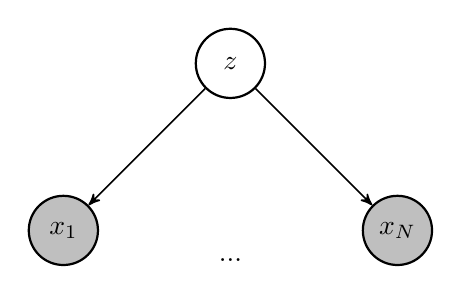
\begin{tikzpicture}[->, >=stealth', auto, semithick, node distance=3cm]
    \tikzstyle{every state}=[fill=white,draw=black,thick,text=black,scale=1]
    \node[state](z){$z$};
    \node[state, fill=lightgray](x1)[below left of=z]{$x_1$};
    \node[above=0.5cm](dots)[below of=z]{$...$};
    \node[state, fill=lightgray](xn)[below right of=z]{$x_N$};
    \path
        (z) edge    node{}    (x1)
            edge    node{}    (xn);
    \end{tikzpicture}
\caption{Graphical model of the MVAE}
\label{fig:mvae_graph}
\end{center}
\end{figure}


The conditional independence assumptions in the generative model (figure \ref{fig:mvae_graph}) imply a relation among joint and single modality posteriors (equation \ref{eq:poe}).

\begin{equation}
    \begin{split}
        p(z|x_1, ..., x_N) & = \frac{p(x_1, ..., x_N | z) p(z)}{p(x_1, ..., x_N)} \\
        & = \frac{p(z)}{p(x_1, ..., x_N)} \prod_{i=1}^{N} p(x_i | z) \\
        & = \frac{p(z)}{p(x_1, ... x_N)} \prod_{i=1}^{N} \frac{p(z|x_i)p(x_i)}{p(z)} \\
        & = \frac{\prod_{i=1}^{N} p(z|x_i)}{\prod_{i=1}^{N-1} p(z)} \frac{\prod_{i=1}^{N}p(x_i)}{p(x_1, ..., x_N)} \\
        & \propto \frac{\prod_{i=1}^{N} p(z|x_i)}{\prod_{i=1}^{N-1} p(z)}
        \approx \frac{\prod_{i=1}^{N} (\widetilde{q}(z|x_i)p(z))}{\prod_{i=1}^{N-1} p(z)}
        = p(z) \prod_{i=1}^{N} \widetilde{q}(z | x_i) \\
        & \text{With $\widetilde{q}(z|x_i)$ the model approximation of $\frac{p(z|x_i)}{p(z)}$}
    \label{eq:poe}
    \end{split}
\end{equation}

Thus, the joint posterior distribution can be approximated by a product of experts (PoE) which includes a \textit{"prior expert"}.

\begin{figure}[h]
    \centering
    \newlength{\MyOtherHeight}
    \settoheight{\MyOtherHeight}{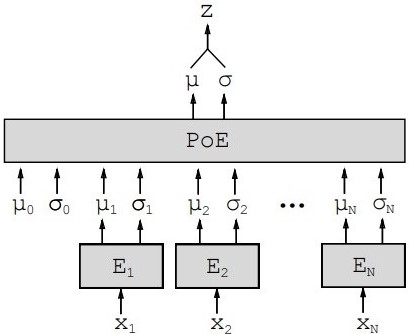
\includegraphics[width=0.9 \textwidth]{images/nn/architectures/mvae_all.jpg}}
    \begin{subfigure}[t]{0.49\textwidth}
        \centering
        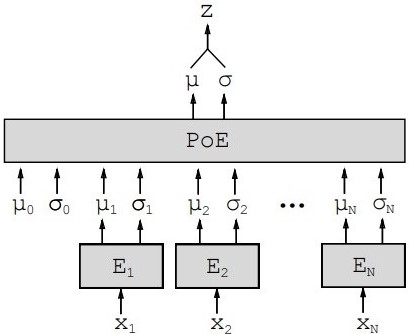
\includegraphics[width=.9 \textwidth]{images/nn/architectures/mvae_all.jpg}
        \caption{With all the modalities}
        \label{fig:mvae_architecture_all}
    \end{subfigure}
    \hfill
    \begin{subfigure}[t]{0.49\textwidth}
        \centering
        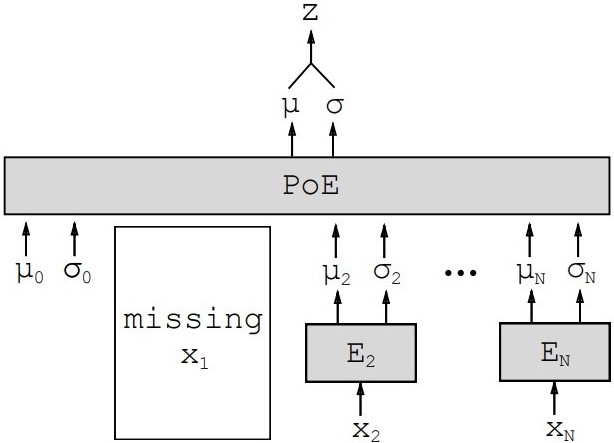
\includegraphics[width=.9 \textwidth]{images/nn/architectures/mvae_missing.jpg}
        \caption{With missing modalities}
        \label{fig:mvae_architecture_missing}
    \end{subfigure}
    \caption{MVAE architecture}
    Source: Mike Wu's paper \cite{wu_multimodal_2018}.
    \label{fig:mvae_architecture}
\end{figure}

The figure \ref{fig:mvae_architecture} and equation \ref{eq:poe} show how the PoE can handle missing modalities by simply ignoring them.

\subsection{Neural Autoregressive Distribution Estimation}
\label{sec:back:nade}

A NADE \cite{uria_neural_2016, uria_deep_2014} is a neural network made to support a $D$-dimensional distribution $p(x)$ which verify the equation \ref{eq:background:nade:eq1}.
\begin{equation}
    p(x) = \prod_{d=1}^{D} p(x_{o_{d}} | x_{o_{<d}})
    \label{eq:background:nade:eq1}
\end{equation}

It is a feed forward network parameterized as in the equations \ref{eq:background:nade:eq2} and \ref{eq:background:nade:eq3}.
\begin{equation}
    p(x_{o_{d}} = 1 | x_{o_{<d}}) = \text{sigm}(V_{o_{d}, .} h_{d} + b_{o_{d}})
    \label{eq:background:nade:eq2}
\end{equation}
\begin{equation}
    h_d = \text{sigm}(W_{., o_{<d}} x_{o_{<d}} + c)
    \label{eq:background:nade:eq3}
\end{equation}
where, with $H$ as the number of hidden units, $V \in \mathbb{R}^{D \times R}$, $b \in \mathbb{R}^{D}$, $W \in \mathbb{R}^{H \times D}$, $c \in \mathbb{R}^{H}$.

The hidden matrix $W$ and bias $c$ are shared by each hidden layer $h_{d}$.
\begin{figure}[ht]
    \centering
    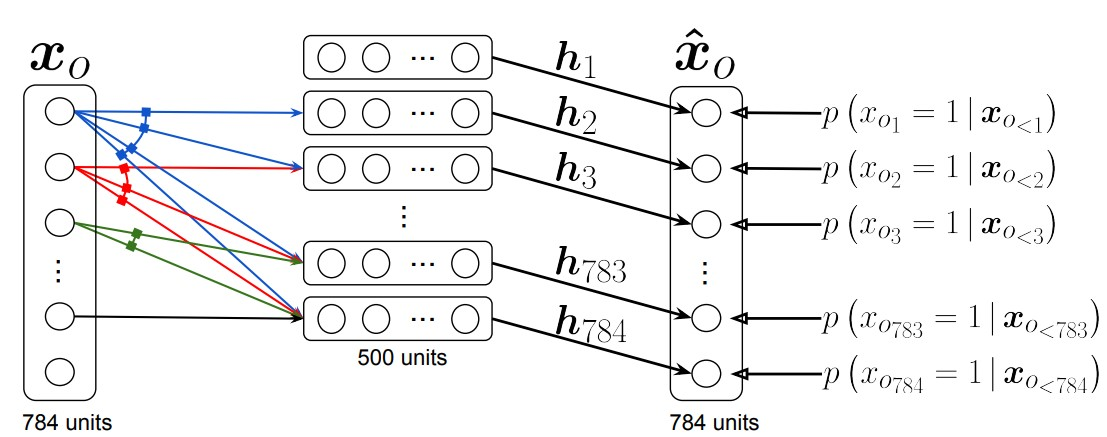
\includegraphics[width=0.8 \textwidth]{images/nn/architectures/nade_architecture.jpg}
    \caption{NADE architectue}
    Source: Benigno Uria et al.'s paper \cite{uria_neural_2016}
    \label{fig:arch:nade}
\end{figure}
The figure \ref{fig:arch:nade} illustrates the Nade model.
There is no path of connections between an output and the value being predicted, or element $x_O$ later in the ordering.
Arrows connected together correspond to connections with shared (tied) parameters.

\subsection{Restricted Bolzmann Machine}
\label{sec:back:rbm}

A RBM is an undirected graphical model \cite{noauthor_restricted_2018, montufar_restricted_2018, salakhutdinov_restricted_2007, fischer_introduction_2012} showed in the figure \ref{fig:arch:rbm}.
As an AE, it encodes the input $x$ in a latent space $h$ where:
\begin{equation}
    h_{i} = \text{sigmoid}(x^{T} W_{i} + a)
\end{equation}
where $x$ is the input, $h$ is the vector corresponding to the hidden layer, $W$ are the weights, $a$ is the hidden layer bias vector.
This is the endoding phase.

For the decoding, or reconstruction phase, the predicted output by the model is:
\begin{equation}
    x^{*}_{i} = \text{sigmoid}(h W^{T} + b)
\end{equation}
where $x^{*}$ is the reconstructed input, $W$ are the same weights as the forward pass, and $b$ are the observed layer bias vector.

\begin{figure}[htbp]
    \centering
    \begin{subfigure}[t]{0.49\textwidth}
        \begin{center}
            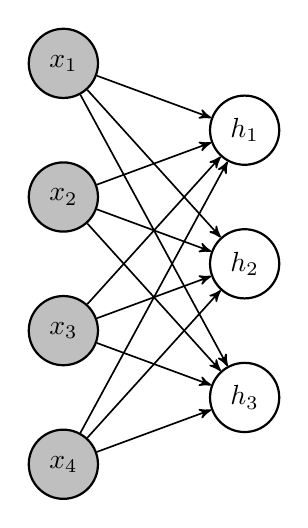
\begin{tikzpicture}[->, >=stealth', auto, semithick, node distance=1.2cm]
            \tikzstyle{every state}=[fill=white,draw=black,thick,text=black,scale=1]
            \node[state, fill=lightgray](x1)[left=1cm]{$x_1$};
            \node[state](h1)[below right of=x1, right=1cm]{$h_1$};
            \node[state, fill=lightgray](x2)[below left of=h1, left=1cm]{$x_2$};
            \node[state](h2)[below right of=x2, right=1cm]{$h_2$};
            \node[state, fill=lightgray](x3)[below left of=h2, left=1cm]{$x_3$};
            \node[state](h3)[below right of=x3, right=1cm]{$h_3$};
            \node[state, fill=lightgray](x4)[below left of=h3, left=1cm]{$x_4$};
            
            \draw (x1) -> (h1);
            \draw (x2) -> (h1);
            \draw (x3) -> (h1);
            \draw (x4) -> (h1);
            \draw (x1) -> (h2);
            \draw (x2) -> (h2);
            \draw (x3) -> (h2);
            \draw (x4) -> (h2);
            \draw (x1) -> (h3);
            \draw (x2) -> (h3);
            \draw (x3) -> (h3);
            \draw (x4) -> (h3);
            \end{tikzpicture}
        \end{center}
        \caption{RBM forward pass}
        \label{fig:rmb_forward}
    \end{subfigure}
    \begin{subfigure}[t]{0.49\textwidth}
        \begin{center}
            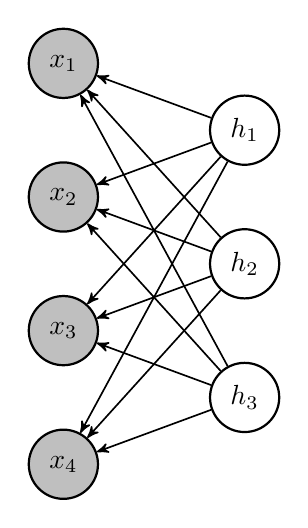
\begin{tikzpicture}[->, >=stealth', auto, semithick, node distance=1.2cm]
            \tikzstyle{every state}=[fill=white,draw=black,thick,text=black,scale=1]
            \node[state, fill=lightgray](x1)[left=1cm]{$x_1$};
            \node[state](h1)[below right of=x1, right=1cm]{$h_1$};
            \node[state, fill=lightgray](x2)[below left of=h1, left=1cm]{$x_2$};
            \node[state](h2)[below right of=x2, right=1cm]{$h_2$};
            \node[state, fill=lightgray](x3)[below left of=h2, left=1cm]{$x_3$};
            \node[state](h3)[below right of=x3, right=1cm]{$h_3$};
            \node[state, fill=lightgray](x4)[below left of=h3, left=1cm]{$x_4$};
            
            \draw (h1) -> (x1);
            \draw (h2) -> (x1);
            \draw (h3) -> (x1);
            \draw (h1) -> (x2);
            \draw (h2) -> (x2);
            \draw (h3) -> (x2);
            \draw (h1) -> (x3);
            \draw (h2) -> (x3);
            \draw (h3) -> (x3);
            \draw (h1) -> (x4);
            \draw (h2) -> (x4);
            \draw (h3) -> (x4);
            
            \end{tikzpicture}
        \end{center}
        \caption{RBM backward pass}
        \label{fig:rmb_backward}
    \end{subfigure}
    \caption{RBM architecture}
    \label{fig:arch:rbm}
\end{figure}

RBMs are Energy-based models and a joint configuration $(x, h)$ has an energy given by:
\begin{equation}
    E(x, h) = -\sum_i a_i x_i - \sum_j b_j h_j - \sum_{(i, j)} x_i h_j w_{ij}
\end{equation}

The probability that the network outputs $x^{*}$ is given by summing over all possible hidden vectors:

\begin{equation}
    p(x^{*}) = \frac{1}{Z} \sum_h e^{- E(x^{*} h)}
\end{equation}
where $Z$ is the partition function:
\begin{equation}
    Z = \sum_{(x,h)} e^{- E(x, h)}
\end{equation}

Training a RBM consists of implementing a gradient descent of the log-likelihood to increase the value of $\log(p(x))$ for $x$ in the dataset.
\begin{equation*}
    \frac{\partial \log(p(x))}{\partial w_{ij}}
\end{equation*}


% ----------------------------------------------------------------------------------------------------
% Related work
% ----------------------------------------------------------------------------------------------------

\chapter{Related works}
\label{chap:related-works}

I will expose in this chapter the works that have already been done about music generation with deep neural networks.
In the section \ref{sec:related-works:objectives}, I will present the different objectives of some implementations.
In the sections \ref{sec:related-works:music-representation} and \ref{sec:related-works:encoding}, I will introduce how the music is represented.
I will then enumerate in the section \ref{sec:related-works:architectures} what architectures have already been used. 
Finally, in the section \ref{sec:related-works:generation-process}, I will illustrate what are the generation processes used.

% -------------------- Objectives  --------------------

\section{Objectives}        % Change the name
\label{sec:related-works:objectives}

In this section, I will describe some examples of what it is possible to do with neural networks to generate music.

As explained in the section \ref{sec:objectives}, my Dissertation's goal is to create a single model able to do as many task as possible a musician or a composer could do.
For instance:
\begin{itemize}
    \item Generate or complete music with several parts (for instance several instruments)
    \item Create a accompaniment from a melody
    \item Create a melody from an accompaniment
    \item Create a musical part from other musical parts
\end{itemize}

\subsection{Generator}

First, it is possible to create a music melody. It can be either monophonic (only one note played at one time) or polyphonic (several notes can be played at the same time).

Secondly, it is possible to create several musical parts at the same time. Each one of them can be either monophonic or polyphonic.
A musical part can be considered as an instrument or voice for a chorale.
The challenge is to create musical parts that work together \cite{donahue_adversarial_2019}.

\subsection{Completion}

The completion challenge is the same as the generation challenge.
The goal is to generate one or several musical parts (they can be either monophonic or polyphonic).
The difference with the generation challenge is that the model takes as an input a \textit{seed}.
The model will continue the musical parts present in the seed.

Completion is the most common objective choice among the existing works \cite{liang_automatic_2017, chuan_modeling_nodate, huang_counterpoint_2017, boulanger-lewandowski_modeling_2012, lattner_imposing_2018}

\subsection{Accompaniment}

Given a melody, or some musical parts, the goal is to create new musical parts which can be combined with the input and be played together \cite{hadjeres_deepbach:_2016, huang_bach_2019}.

This is for example the goal of DeepBach from Gaëtan Hadjeres et al.'s paper \cite{hadjeres_deepbach:_2016}.

Bach Doodle \cite{huang_bach_2019} is an online tool developed by Google.
Users can create their own melody and have it harmonized by a model in the style of Bach.
The figure \ref{fig:bachdoodle} shows the view of this application.
The black melody is the melody entered by the user (me) and Bach Doodle created the accompaniment (red, green and blue melodies).

\begin{figure}[htbp]
    \centering
    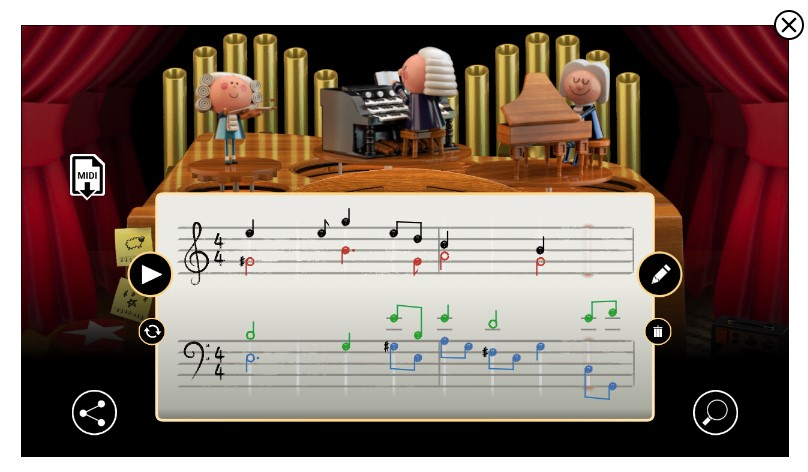
\includegraphics[width=\textwidth]{images/related_works/bachdooldle/bachdoodle.jpg}
    \caption{Bach Doodle application}
    Source: \href{https://www.google.com/doodles/celebrating-johann-sebastian-bach}{BachDoodle}
    \label{fig:bachdoodle}
\end{figure}

% -------------------- Music Representation--------------------

\section{Music Representation}
\label{sec:related-works:music-representation}

In this section, I will present different types of inputs the related works use.

\subsection{Audio Signal} 

The first data used to create music is the audio signal. Some works \cite{oord_wavenet:_2016, dieleman_challenge_2018, donahue_adversarial_2019, kalchbrenner_efficient_2018, mehri_samplernn_2017, lu_play_2018} have been done to generate music audio signal.
This signal can be represented either by its waveform \cite{oord_wavenet:_2016}, its Fourier Transform, or its spectrogram (figures \ref{fig:waveform_example}, \ref{fig:spectrogram_example}).

\begin{figure}[H]
   \begin{minipage}{0.5\textwidth}
     \centering
     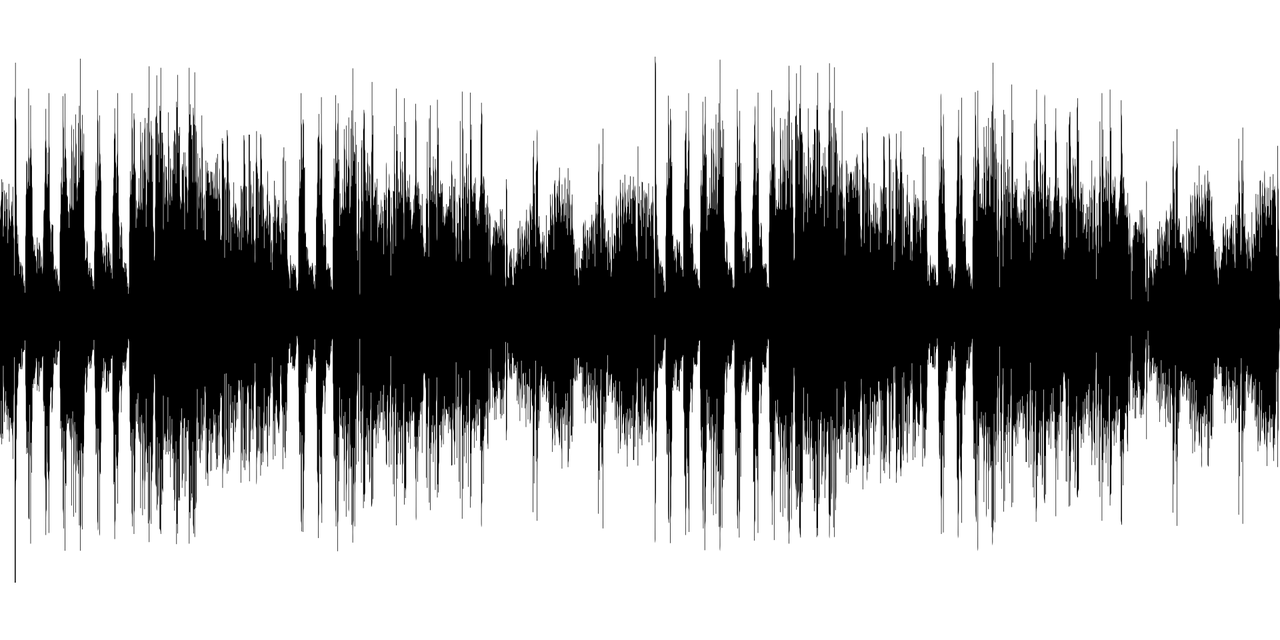
\includegraphics[width=.9\linewidth, height=4cm]{images/music/waveform/waveform.png}
     \caption{Example of an audio waveform}
     Source: \href{https://www.needpix.com/photo/856116/audio-aural-ear-hearing-music-musical-recording-silhouette-sonic}{Needpix.com}
     \label{fig:waveform_example}
   \end{minipage}\hfill
   \begin{minipage}{0.5\textwidth}
     \centering
     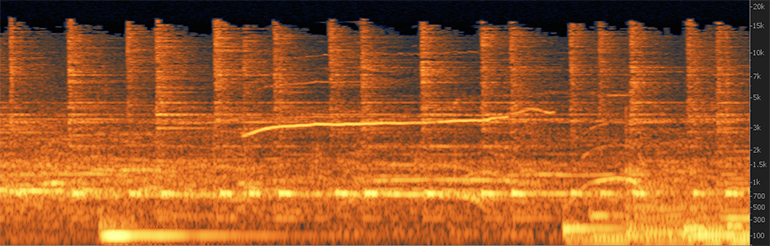
\includegraphics[width=\linewidth, height=4cm]{images/music/spectrogram/izotope-spectrogram.png}
     \caption{Example of audio spectrogram}
     Source: iZotope's tutorial \cite{noauthor_understanding_nodate} %\href{https://commons.wikimedia.org/wiki/File:Spectrogram_of_Bach\%27s_Chorales_for_Organ.jpg}{Wikipedia}
     \label{fig:spectrogram_example}
   \end{minipage}
\end{figure}

Using the audio signal allows the model to handle every aspects of the song at the same time (instrument, timber, emotion...), and every song in the same way.
The biggest issue of this method is that the number of points needed to create a waveform is incredibly huge.
The usual sampling frequency is $48kHz$. 
Therefore, the main difficulty is to stay consistent through time.

\subsection{MIDI Signal}

Most of the works done on music generation use the \textit{MIDI} representation (or any other translation of midi like pianoroll or text). \cite{chuan_modeling_nodate, hadjeres_deepbach:_2016, huang_counterpoint_2017, liang_automatic_2017, adiloglu_machine_2007, herremans_composing_2013, herremans_modeling_2017, boulanger-lewandowski_modeling_2012, lattner_imposing_2018, colombo_learning_2019, brunner_symbolic_2018, wu_hierarchical_2018}

\subsubsection{Pianoroll}
\label{sec:rw:pianoroll}

The pianoroll representation can be considered as an image.
Thus, usual deep learning methods on images can  be applied \cite{huang_counterpoint_2017, chuan_modeling_nodate, boulanger-lewandowski_modeling_2012, lattner_imposing_2018, donahue_adversarial_2019}.
The figure \ref{fig:pianoroll_to_array} shows a very simple example of how to convert a pianoroll view to an array.

\begin{figure}[H]
   \begin{minipage}{0.5\textwidth}
     \centering
     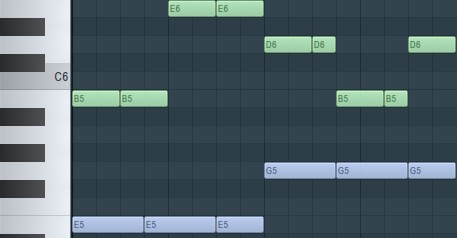
\includegraphics[width=.9\linewidth]{images/music/pianoroll/pianoroll_small.jpg}
   \end{minipage}\hfill
   \begin{minipage}{0.5\textwidth}
     \centering
     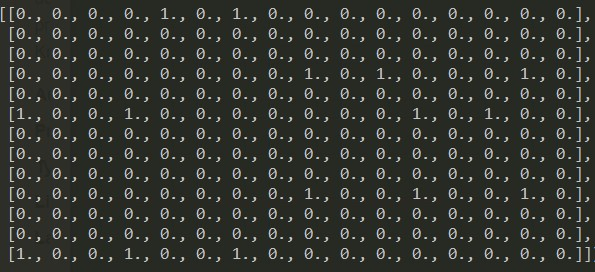
\includegraphics[width=\linewidth]{images/music/pianoroll/pianoroll_small_array.jpg}
   \end{minipage}
 \caption{Example of correspondence between a pianoroll representation and an array}
 \label{fig:pianoroll_to_array}
\end{figure}

\bigskip

Chin-Hua Chuan et al. \cite{chuan_modeling_nodate} introduced another representation to help the model to understand relations between notes.
They use \textit{Tonnetz} matrix \cite{mason_essential_nodate} to represent polyphonic music.
As explained in their paper, \textit{"Tonnetz is a graphical representation used by music theorists and musicologists in order to study tonality and tonal spaces"}.

Instead of encoding notes in a one-dimensional tensor (figure \ref{fig:tonnetz}), they encode them in a 2-dimensional tensor where the relative positions between two notes is meaningful.

The figure \ref{fig:tonnetz} illustrates a common form of tonnetz.
In the tonnetz network, each node represents one of the 12 pitch classes.
The nodes on the same horizontal line follow the Fifth circle ordering. Two adjacent nodes on the horizontal line is a Fourth or Fifth interval
An upside-down triangle filled with diagonal lines in the figure \ref{fig:tonnetz} is $C$ major chord, and the solid triangle on the top is $C$ minor chord.

In Chuan's paper, they extended this matrix.
The figure \ref{fig:tonnetz_extended} shows an extended tonnetz matrix example.
They include to this extended matrix the pitch (octave number) which was missing in the first one.

\begin{figure}[h]
    \centering
    \newlength{\MyOtherHeightThree}
    \settoheight{\MyOtherHeightThree}{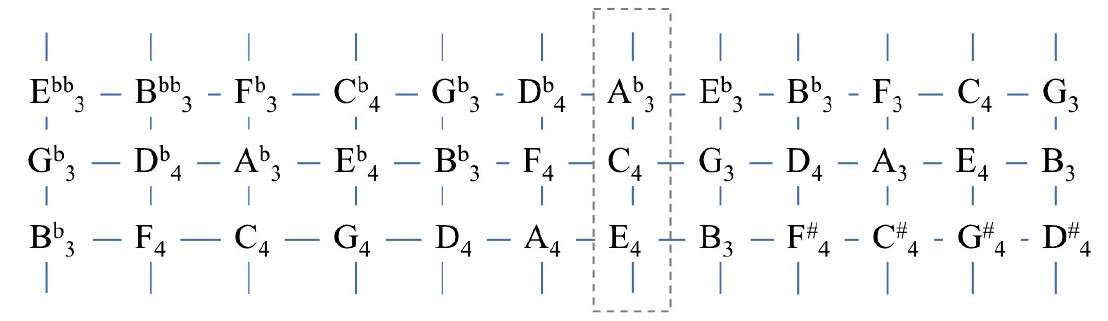
\includegraphics[width=0.9 \textwidth]{images/music/pianoroll/tonnetz_extended.jpg}}
    \begin{subfigure}[t]{0.38\textwidth}
        \centering
        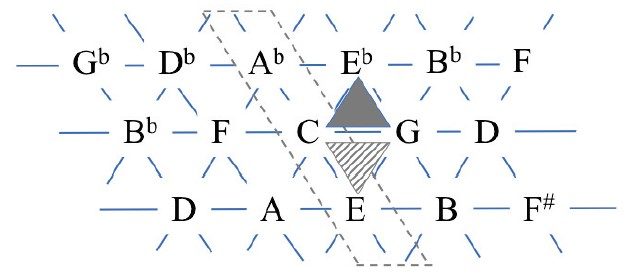
\includegraphics[width=\textwidth]{images/music/pianoroll/tonnetz.jpg}
        \caption{}
        \label{fig:tonnetz}
    \end{subfigure}
    \hfill
    \begin{subfigure}[t]{0.6\textwidth}
        \centering
        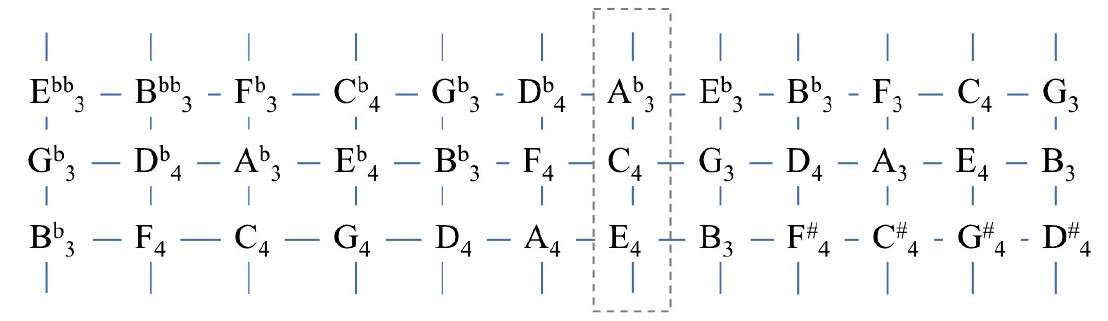
\includegraphics[width=\textwidth]{images/music/pianoroll/tonnetz_extended.jpg}
        \caption{}
        \label{fig:tonnetz_extended}
    \end{subfigure}
    \caption{(a) tonnetz and (b) the extended tonnetz matrix with pitch register}
    Source: Ching-Hua Chuan's paper \cite{chuan_modeling_nodate}.
    \label{fig:tonnetz_representation}
\end{figure}

\subsubsection{Text}
\label{sec:rw:midi:text}

Another approach is to convert the MIDI format into text. \cite{hadjeres_deepbach:_2016}

\begin{figure}[H]
   \begin{minipage}{0.5\textwidth}
     \centering
     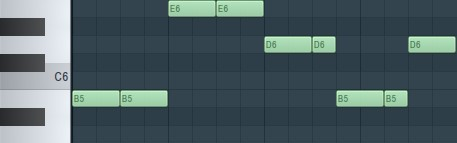
\includegraphics[width=.9\linewidth]{images/music/pianoroll/pianoroll_small_2.jpg}
   \end{minipage}\hfill
   \begin{minipage}{0.5\textwidth}
     \centering
     B5, \_, B5, \_, E6, \_, E6, \_, D6, \_, D6, B5, \_, B5, D6, \_ 
   \end{minipage}
 \caption{Example of correspondence between a pianoroll representation and a text}
 \label{fig:pianoroll_to_text}
\end{figure}

The figure \ref{fig:pianoroll_to_text} shows a simple example of how it is possible to convert an pianoroll view to a text.
However, using text to represent a pianoroll usually forces the framework to work only in a monophonic way.
A common choice of the existing works that work with text is to embed the text into a fix-sized vector using a \texttt{word2vec} \cite{goldberg_word2vec_2014, karani_introduction_2018, rong_word2vec_2016, noauthor_beginners_nodate, mikolov_distributed_2013} model \cite{liang_automatic_2017, herremans_modeling_2017}.

\bigskip

Despite the text constraints, Feynman Liang and al. \cite{liang_automatic_2017} managed to encode polyphonic music in text and use it to correctly train their model: \textit{"BachBot"}.

They quantize time into sixteenth notes (\musEighth). Consecutive frames are separated by a unique delimiter ("\texttt{|||}").
Within each frame, they represent individual notes rather than entire chords.
Each frame consists of four (Soprano, Alto, Tenor, and Bass) \texttt{<Pitch; Tie>} tuples where $\texttt{Pitch} \in \{0; 1; \dots ; 127\}$ represents the MIDI pitch of a note and $\texttt{Tie} \in \{\texttt{True}; \texttt{False}\}$ distinguishes whether a note is tied with a note at the same pitch from the
previous frame or is articulated at the current timestep.
They \textit{order notes within a frame in descending MIDI pitch}.
The figure \ref{fig:relatedwork_bachbot} shows the encoding process.

\begin{figure}[h]
    \centering
    \newlength{\MyOtherHeightTwo}
    \settoheight{\MyOtherHeightTwo}{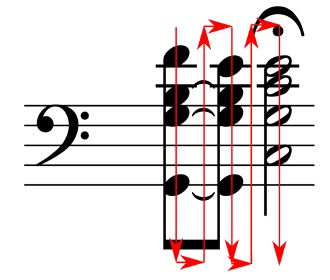
\includegraphics[width=0.9 \textwidth]{images/related_works/bachbot/bachbot_encoding_stave.jpg}}
    \begin{subfigure}[t]{0.28\textwidth}
        \centering
        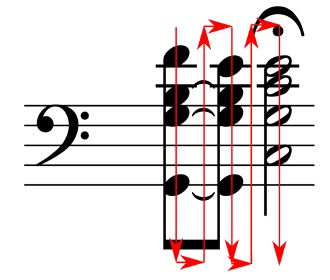
\includegraphics[width=.9 \textwidth]{images/related_works/bachbot/bachbot_encoding_stave.jpg}
        \caption{ {\setstretch{1.}Three musical chords in traditional music notation. The red arrows indicate the order in which notes are sequentially encoded.}}
        \label{fig:relatedwork_bachbot_stave}
    \end{subfigure}
    \hfill
    \begin{subfigure}[t]{0.67\textwidth}
        \centering
        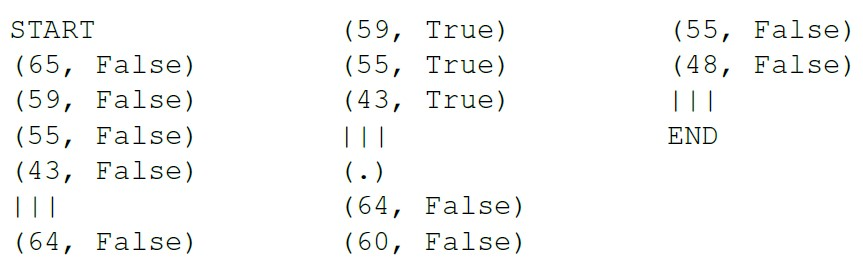
\includegraphics[width=.9 \textwidth]{images/related_works/bachbot/bachbot_encoding_text.jpg}
        \caption{A corresponding sequential encoding of the three chords in an eighth-note time quantization (for illustration, broken over three columns). Each line within a column corresponds to an individual token in the encoded sequence. ||| delimit frames and (.) indicate a fermata is present within the corresponding frame.}
        \label{fig:relatedwork_bachbot_text}
    \end{subfigure}
    \caption{BachBot's example encoding of three musical chords ending with a fermata ("pause") chord}
    Source: Feynman Lian's paper \cite{liang_automatic_2017}.
    \label{fig:relatedwork_bachbot}
\end{figure}


\subsubsection{Chords}

This is the last approach I will describe in this paper.
As the same way as Jazz music, it is possible to simplify the description of a musical piece by writing down the chords.

\begin{figure}[H]
   \begin{minipage}{0.5\textwidth}
     \centering
     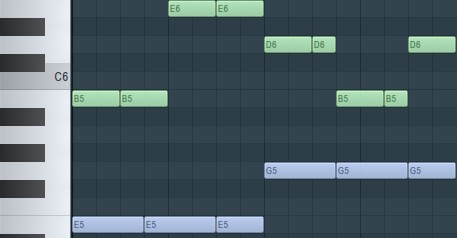
\includegraphics[width=.9\linewidth]{images/music/pianoroll/pianoroll_small.jpg}
   \end{minipage}\hfill
   \begin{minipage}{0.5\textwidth}
     \centering
     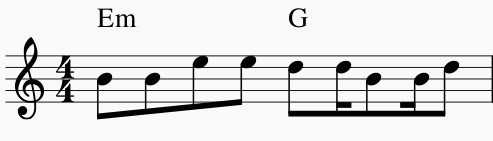
\includegraphics[width=.9\linewidth]{images/music/stave/stave_with_chords.jpg}
   \end{minipage}
 \caption{Example of correspondence between a pianoroll and its chords representation}
 \label{fig:pianoroll_to_chords}
\end{figure}

For instance, in the figure \ref{fig:pianoroll_to_chords}, the bass line can be simplified by considering the chords.
The chords are then written and be considered as notes.

% -------------------- Encoding --------------------

\section{Encoding}
\label{sec:related-works:encoding}

\subsection{Features}

It is possible to extract features from the data to help the neural network to understand how music works, like the chords, the current key signature...
\begin{itemize}
    \item The first option is to do it manually and give the features as an input of the model
    \item The second option is to let the model learn it by itself. This is the choice I have made for this project.
\end{itemize}

\subsubsection{Metadata}

The features that can be passed as an input to the model can also be metadata like the time signature or the key of the music...

Deep Bach from Gaëtan Hadjeres et al.'s paper \cite{hadjeres_deepbach:_2016} considers the fermata symbol (figure \ref{fig:fermata}) and the beat subdivision number (an integer between 1 and 4).

\begin{figure}[htbp]
     \centering
     
\includegraphics[width=.1\linewidth]{images/music/symbols/fermata.png}
     \caption{Fermata symbol}
     Source: \href{https://publicdomainvectors.org/en/free-clipart/Music-symbol/70183.html}{publicdomainvector}
     \label{fig:fermata}
\end{figure}

In this project I chose to not include any metadata in the model because of the difficulty to find or reconstruct them for the available dataset.
However, I give to the model the information about the beats number and subdivisions by considering the entire measure as one entire object or step.

\bigskip

Another way to help the model by giving it information without actually passing metadata is to normalize the data.
For example, BachBot \cite{liang_automatic_2017} and other works \cite{chuan_modeling_nodate, boulanger-lewandowski_modeling_2012} transpose all their dataset in either $C$ major or $A$ minor key.

For the same reason as not passing metadata, I didn't normalize the data before training my models.
However, because I was having poor results, I decided afterward to transpose all the song sin either the $C$ major scale or the $A$ minor scale.

\subsection{Tensor encoding}

It is possible to extract two different methods on how to encode the tensor which will be given to the neural network

The first method is the \textit{value encoding}.
It means that the values in the input and/or output tensor are actually meaningful.
For example, it can be an integer which is the pitch of a note.

The second method is called \textit{item encoding}.
Instead of having the number of the pitch in the tensor (let's say $60$), it will be a very sparse tensor with a bunch on $0$ and a $1$ at the position $60$ in the pitch dimension.
This values stored in the tensors can be considered as \textit{activation} values.
This is the retained method in my Dissertation.


\section{Architectures}
\label{sec:related-works:architectures}


In this section, I will present different architectures that have already been used for music generation. It will expose the architecture of my project in the section \ref{sec:rmvae}.


\subsection{RBM}

The RBM architecture is explained in the section \ref{sec:back:rbm}.

Nicolas Boulanger-Lewandowski et al. \cite{boulanger-lewandowski_modeling_2012} use an RBM based model RTRBM \cite{sutskever_recurrent_nodate, mittelman_structured_nodate} and created their own architecture called RNN-RBM.
They applied their model on different MIDI dataset to create polyphonic music.

Stefan Lattner et al. \cite{lattner_imposing_2018} use another RBM based model called C-RBM \cite{norouzi_convolutional_nodate, norouzi_stacks_nodate}.
They apply this model on pianoroll images.
They also implement a different constraints like their self-similarity constraint to specify a repetition structure (e.g. AABA) in the general music piece.


\subsection{NADE}
\label{sec:rw:nade}

The NADE architecture is explained in the section \ref{sec:back:nade}.

And as an example, Cheng-Zhi Anna Huang et al. \cite{huang_counterpoint_2017} use an orderless NADE \cite{uria_deep_2014} to generate music. They introduce COCONET, a deep convolutional model to reconstruct partial scores.
It consists of a corruption process that masks out a subset $x_{\neg C}$ of variables, followed by a process that independently resamples variables $x_{i}$ (with $i \not \in C$) according to the distribution $p_{\theta} (x_i | x_C )$ emitted by the model with parameters $\theta$.


The figure \ref{fig:coconet_process} illustrates how the process works.
At each step, a random subset of notes is removed, and the model is asked to infer their values.
New values are sampled from the probability distribution put out by the model, and the process is repeated.

Google also created Bach Doodle \cite{huang_bach_2019}, an online tool re-implementing COCONET in Tensorflow.js \cite{noauthor_tensorflowjs_nodate} which harmonizes a melody given by the user.


\subsection{AE}

The AutoEncoder architecture is explained in the section \ref{sec:back:ae}.

This is the most common architecture used for music generation at the time I am writing this report.
The AutoEncoder can be recurrent  \cite{liang_automatic_2017, chuan_modeling_nodate, hadjeres_deepbach:_2016, kalchbrenner_efficient_2018, mehri_samplernn_2017} as Feynman Liang et al.'s BachBot \cite{liang_automatic_2017} or not \cite{dieleman_challenge_2018}.

For instance, BachBot \cite{liang_automatic_2017} and DeepBach \cite{hadjeres_deepbach:_2016} use an encoder/decoder architecture with LSMT layers on the latent space. \cite{chuan_modeling_nodate}

Soroush Mehri et al. \cite{mehri_samplernn_2017} or Nal Kalchbrenner et al. \cite{kalchbrenner_efficient_2018} have created different AE architecture to synthesize audio waveform and can be applied to music sounds.

\subsection{VAE}

The Variational AutoEncoder architecture is explained in the section \ref{sec:back:vae}. 

Sander Dieleman et al. \cite{dieleman_challenge_2018} use a VAE (or more precisly a VQ-VAE \cite{van_den_oord_neural_2017}  or a AMAE \cite{dieleman_challenge_2018}) to encode audio waveform and reconstruct it with a stylistic consistency accross tens of seconds.



\subsection{GAN}

The Generative Adversarial Network architecture is explained in the section \ref{sec:back:gan}

For instance, the model WaveGan from Chris Donahue et al. \cite{donahue_adversarial_2019} use a GAN architecture to synthesize audio waveform in several domains including drums and piano.

Gino Brunner et al. \cite{brunner_symbolic_2018} use CycleGAN \cite{zhu_unpaired_2018} to create a model able to apply a style transfer on musical pieces (between jazz, pop and classical style).

\subsection{Transformers}

The Transformer's architecture is explained in the section \ref{sec:back:transformers}.
Some works have already been done on music generation with Transformers as, for instance, Cheng-Zhi Anna Huang et al. \cite{huang_music_2018} and Kristy Choi et al. \cite{choi_encoding_2019}.

Huang et al. introduce the Music Transformer, a model able to generate consistent samples longer than samples generated by a RNN architecture.
They achieve this perfomance by using a Transformer with relative attention (equation \ref{eq:relative-attention}).

\begin{equation}
    \text{RelativeAttention} = \text{Softmax} (\frac{QK^T + S^{rel}}{\sqrt{D_h}})V
    \label{eq:relative-attention}
\end{equation}

\section{Generation Process}
\label{sec:related-works:generation-process}

In this section, I will enumerate different techniques to generate music from different model architectures.

\subsection{Sampling}

The sampling process can either be done with a VAE, or an GAN architecture \cite{donahue_adversarial_2019}.

A VAE keeps its latent space distribution as close as the standard normal distribution $\mathcal{N}(0, 1)$.
Thus, by giving a random vector sampled from a standard normal distribution $\mathcal{N}(0, 1)$, the decoder will construct an output similar to the dataset the model trained on.

The generator of a GAN has been trained to generated consistent data from noise.
Then, the process generation for a GAN is to give a random input from a standard normal distribution to generator.

\subsection{Input Manipulation}

Generating music by manipulating the input is typically how style transfer algorithms work \cite{shetty_neural_2019, gatys_neural_2015, li_universal_2017}.
The input is considered as a variable which is updated to minimize a loss function constructed from a content target and a style target.
The content similarities between the input and the content target is reduced through iterations.
In the same way, the style similarities between the style target and the input will be minimized.

This process works well for images to create a new image combining content and style from 2 different images.
People tried to apply the same methods on music \cite{kaliakatsos-papakostas_conceptual_2017, hung_musical_2019, brunner_symbolic_2018, lu_play_2018}.
However, as Shuqi et al. \cite{dai_music_2018} say, music is more complex and has several level of style (timber, performance and composition).
Therefore, creating a music style transfer algorithm is more complicated than for images and the results are currently not as good.

\subsection{Feed forward and RNN architecture}
\label{sec:rw:feed-forward}

This is the easiest and most common generation process through all the works \cite{liang_automatic_2017, chuan_modeling_nodate, huang_counterpoint_2017, wu_hierarchical_2018}, and this is the one I chose for this project.
An input is given to the model and the model returns an output.
The figure \ref{fig:feed_forward_generation_process} illustrates this process.
This output can be the next frame/beat/measure of the music.

In my case, the model returns the next measure of the music.

\begin{figure}[h]
\begin{center}
    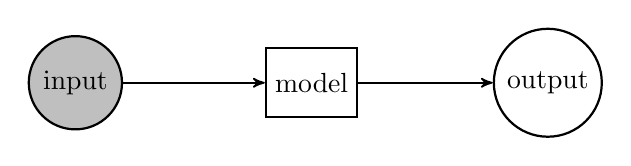
\begin{tikzpicture}[->, >=stealth', auto, semithick, node distance=3cm]
    \tikzstyle{every state}=[fill=white,draw=black,thick,text=black,scale=1]
    \node[state, rectangle](model){model};
    \node[state, fill=lightgray](input)[left of=model]{input};
    \node[state](output)[right of=model]{output};
    \path
        (input) edge    node{}  (model)
        (model) edge    node{}  (output);
    \end{tikzpicture}
\caption{Feed forward generation process}
\label{fig:feed_forward_generation_process}
\end{center}
\end{figure}

\subsubsection{DeepBach}

To give an illustration, DeepBach \cite{hadjeres_deepbach:_2016} uses a Markov Chain Monte Carlo algorithm to re-harmonize a song and transform it. 
From the existing song, it re-predicts every notes one by one.
The algorithm is describe in the figure \ref{fig:relatedworks:deepbach_architecture}.

\begin{figure}[htbp]
     \centering
     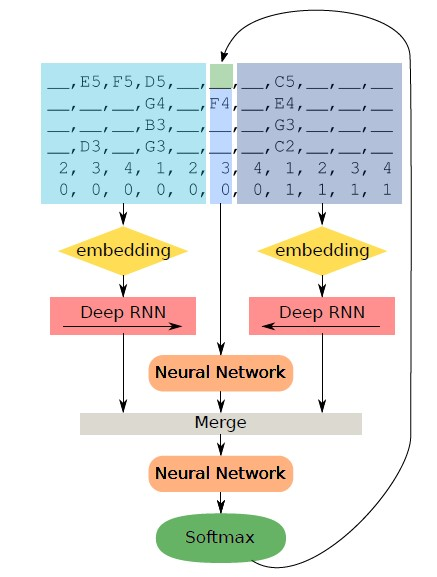
\includegraphics[width=.5\linewidth]{images/related_works/deepbach/deepbach_algo.jpg}
     \caption{Graphical representation of DeepBach's neural network architecture for the soprano prediction}
     Source: DeepBach paper \cite{hadjeres_deepbach:_2016}
     \label{fig:relatedworks:deepbach_architecture}
\end{figure}

\section{Thesis contributions and relation to prior work}

As explained in the introduction, I aim to create only one model which can handle several tasks as:
\begin{itemize}
    \item Generate or complete music with several musical parts (meaning several instruments)
    \item Create a accompaniment from a melody
    \item Create a melody from a accompaniment
    \item Create a musical part from other musical parts
\end{itemize}

Unfortunately, the related works don't have a such objective and the used neural architectures couldn't fit my needs.
That is why I created a new architecture called Recurrent Multimodal Variational AutoEncoder.
This architecture is explained in the section \ref{sec:rmvae}.

Because of the difficulty of obtaining clean data and of extracting meta data from a musical score, I decided to not work on that part and mostly focus my efforts on the deep learning part.
However, the results I obtained didn't satisfied me.
That is why I decided to transpose all the songs from my datasets in the $C$ major key or the $A$ minor key.

I decided to use the pianoroll representation (section \ref{sec:rw:pianoroll}) because this is how I (as a pianist) personally visualize the music).
And I chose to consider the measure as an entire object (and not a frame) because this is how I conceptualize music.

Finally, all along my project, I had the hope to be able to play and jam with a trained model, that is why I chose my generation process to be feed-forward (section \ref{sec:rw:feed-forward}).
This is the simplest way to consider the notes I play and build a real time application.

% ----------------------------------------------------------------------------------------------------
% Contribution
% ----------------------------------------------------------------------------------------------------
\newpage
\chapter{Contribution: Multi-Modal Music Generation}
\label{chap:contribution}

I will explain in this chapter what have been my original works for my Dissertation.
In the section \ref{sec:objectives}, I will explain what I have been aiming to do.
In the section \ref{sec:data_represetation}, I will explain how I decided to represent the data and how I decided to work with it.
In the section \ref{sec:rmvae}, I will describe my novel architecture (RMVAE) that I have created for my Dissertation.
In the section \ref{sec:loss}, I'll illustrate how I gave some prior knowledge to the network with custom loss functions.
And finally, in the section \ref{sec:learning-process}, I will explain how the RMVAE is trained and how it can be used to create a new song.

% -------------------- Objectives --------------------

\section{Objectives}
\label{sec:objectives}

As a musician, I wanted to create a model architecture who could copy the way I think about music.
The challenge is to use only one trained model to be able to:
\begin{itemize}
    \item Generate or complete music with several musical parts (meaning several instruments)
    \item Create a accompaniment from a melody
    \item Create a melody from a accompaniment
    \item Create a musical part from other musical parts
\end{itemize}
The created model can also handle missing data (for example a missing measure from an instrument).

To summarize, the objective is to create a unique trained model which can generate or arrange a musical piece whatever is already present or missing.

\section{Data representation}
\label{sec:data_represetation}

This project works with MIDI data. This music representation is explained in the section \ref{sec:midi}. \\
The shortest beat division is a quarter of a beat (sixteenth note: \musSixteenth) \\
The considered music are binary and with 4 beats per measure. \\
Because I think that a measure can be considered as an entire object (with its rhythm, its chords ...), I chose to divide music by measure. Thus, a time step for the neural network is the representation of an entire measure.
The shape of a tensor representing a measure will be \texttt{(16, 128, channels)}:
\begin{itemize}
    \item \texttt{16} is the number of sixteenth notes (\musSixteenth) is a measure.
    \item \texttt{128} is the number of different MIDI notes possible (from $0$ to $127$).
    \item \texttt{channels} $\in \{1, 2\}$ is explained in the sections \ref{sec:poly} and \ref{sec:mono}.
\end{itemize}

The number of instruments is fixed and are different inputs of the neural network.
Hence, for one instrument, its associated tensor has a shape of \texttt{(nb\_measures, 16, 128, channels)}. \texttt{nb\_measures} is the number of measures considered to predict the next one.

\subsection{Polyphonic music}
\label{sec:poly}

For polyphonic music, the number of \texttt{channels} it $2$.

The first channel is called the \textit{activation} channel. The value is either $1$ for a played note or $0$ for a non-played note.

The second channel is called the \textit{duration} channel. The value is an integer corresponding of \textit{"how many sixteenth notes (\musSixteenth) it lasts"}.
The table \ref{tab:duration} shows the correspondence between the value of the duration channel and the musical length representation.

\begin{table} [ht]
    \begin{center}
        \begin{tabular} {c|c}
            Duration value & Musical length \\
            \hline
            $1$ & \musSixteenth \\
            $2$ & \musEighth \\
            $3$ & \musEighthDotted \\
            $4$ & \musQuarter \\
            $5$ & $\musQuarter_{\smile}$\musSixteenth \\
            $6$ & \musQuarterDotted \\
            $7$ & $\musQuarter_{\smile} \musEighthDotted$ \\
            $8$ & \musHalf \\
            $9$ & $\musHalf_{\smile} \musSixteenth$ \\
            $10$ & $\musHalf_{\smile} \musEighth$ \\
            $11$ & $\musHalf_{\smile} \musEighthDotted$ \\
            $12$ & \musHalfDotted \\
            $13$ & $\musHalfDotted_{\smile} \musSixteenth$ \\
            $14$ & $\musHalfDotted_{\smile} \musEighth$ \\
            $15$ & $\musHalfDotted_{\smile} \musEighthDotted$ \\
            $16$ & \musWhole \\
        \end{tabular}
        \caption{Correspondence between duration value and musical length}
        \label{tab:duration}
    \end{center}
\end{table}

If a note is not activated (activation channel $ = 0$), then the duration channel is set to $0$ too.

\begin{equation}
    \texttt{channel}_{\texttt{activation}} = 0 \iff \texttt{channel}_{\texttt{duration}} = 0
\end{equation}

\subsection{Monophonic Music}
\label{sec:mono}

The goal was too reduce the memory space and simplify the model for monophonic music.
Since monophonic music means there is a maximum of one note played simultaneously at one time $t$, I chose to not consider musical rests and consider that every notes last until the next note is played.\\
Thus, I deleted the duration channel.
Now, the number of $\texttt{channels} = 1$.

An \textit{additional note} is inserted which is the $note_{continue}$.
The tensor shape of a step is now \texttt{(16, 128 + 1, 1)}.
When $note_{continue}$ is set to $1$, it means there is no new note to be played.
And when $note_{continue}$ is set to $0$, it means a new notes has to be played.

\begin{equation}
    note_{continue} = 1 \implies \forall~ note \in notes_{[0:128]}, note = 0
\end{equation}

\begin{equation}
    note_{continue} = 0 \implies \exists!~ note \in notes_{[0:128]}, note = 1
\end{equation}

And since I consider in this part only monophonic music, there is only on note (included $note_{continue}$ per each time division).

\begin{equation}
    \exists! note \in notes_{[0:129]}, note = 1
\end{equation}

% -------------------- Architecture --------------------

\section{RMVAE Architecture}
\label{sec:rmvae}

I have created a new architecture which is able to handle all the objectives defined in the section \ref{sec:objectives}.

To do so, I continued the work of Mike Wu et al. \cite{wu_multimodal_2018} and their Multimodal Varational AutoEncoder (MVAE) (see section \ref{sec:back:mvae}) and I simplified the work of Tan Zhi-Xuan et al. \cite{tan_factorized_2019} and their Multimodal Deep Markov Models (MDMM).

\subsection{Global Architecture}

I use the capability of the MVAE to reconstruct data and handle several modalities at the same time with the help of the product of expert operation.
But because the MVAE doesn't handle time across the data, it had to be transformed.
And that is basically what does the MDMM.
However, the training process of a MDMM is quite complicated and slow.
Because of this, I came up with a novel architecture that I call RMVAE (Recurrent Multimodal Varational AutoEncoder).
This architecture is described in the figure \ref{fig:rmvae_architecture}.


% Good example how to use tikz:
% https://tex.stackexchange.com/questions/193694/drawing-graph-of-markov-chain-with-patches-using-tikz
\begin{figure}
\begin{center}
    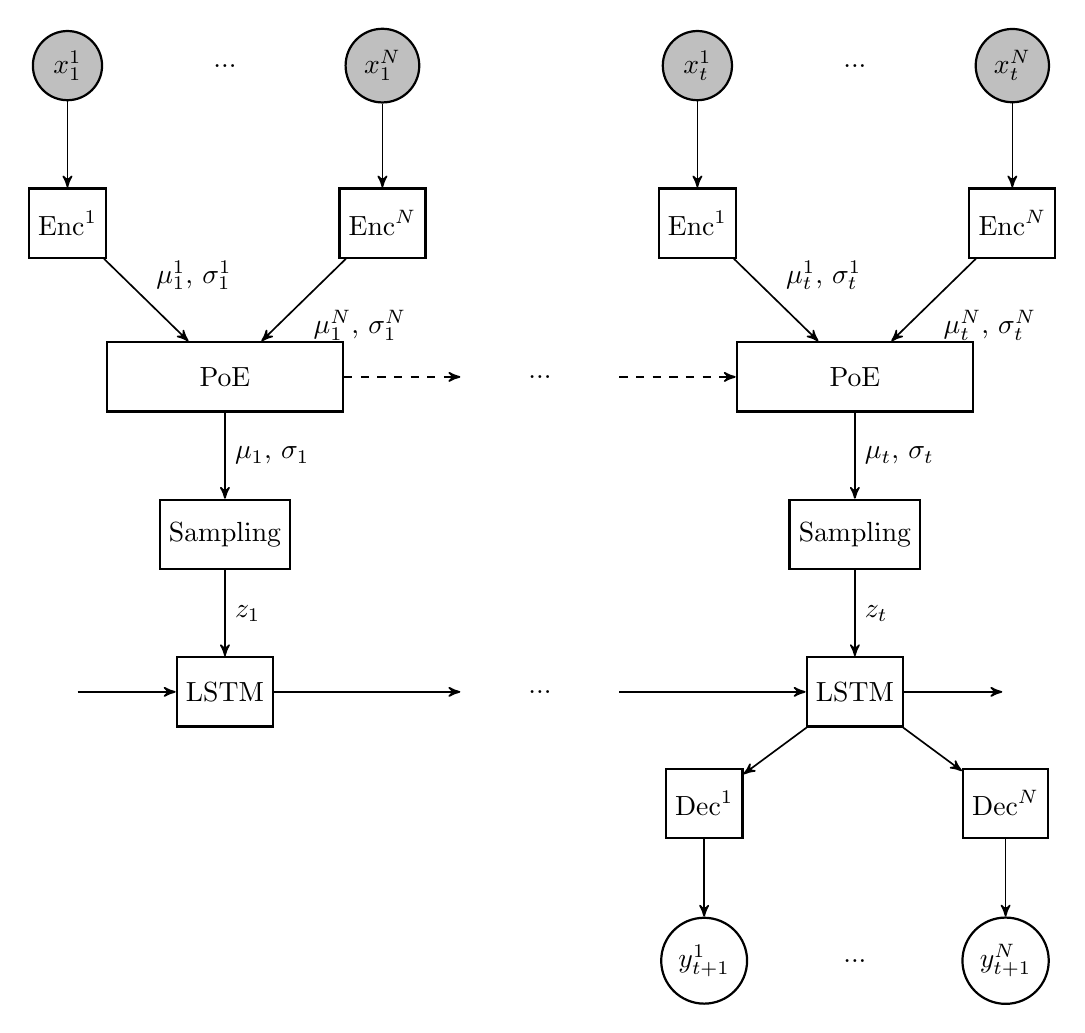
\begin{tikzpicture}[->, >=stealth', auto, semithick, node distance=2cm]
    \tikzstyle{every state}=[fill=white,draw=black,thick,text=black,scale=1]
    \node[state, fill=lightgray](x11)[]{$x_1^1$};
    \node[](dots1)[right of=x11]{$...$};
    \node[state, fill=lightgray](x1n)[right of=dots1]{$x_1^N$};
    \node[state, rectangle](enc11)[below of=x11]{$\text{Enc}^1$};
    \node[state, rectangle](enc1n)[below of=x1n]{$\text{Enc}^N$};
    \node[state, rectangle, below=1.5cm, minimum width=3cm](poe1) at ($(enc11)!0.5!(enc1n)$) {PoE};
    \node[state, rectangle](samp1)[below of=poe1]{Sampling};
    \node[state, rectangle](lstm1)[below of=samp1]{LSTM};
    
    \node[state, fill=lightgray, right=2cm](xt1)[right of=x1n]{$x_t^1$};
    \node[](dots2)[right of=xt1]{$...$};
    \node[state, fill=lightgray](xtn)[right of=dots2]{$x_t^N$};
    \node[state, rectangle](enct1)[below of=xt1]{$\text{Enc}^1$};
    \node[state, rectangle](enctn)[below of=xtn]{$\text{Enc}^N$};
    \node[state, rectangle, below=1.5cm, minimum width=3cm](poet) at ($(enct1)!0.5!(enctn)$) {PoE};
    \node[state, rectangle](sampt)[below of=poet]{Sampling};
    \node[state, rectangle](lstmt)[below of=sampt]{LSTM};
    
    \node[minimum width=2cm](lstmdots) at ($(lstm1)!0.5!(lstmt)$) {...};
    
    \node[](lstm0)[left of=lstm1]{};
    \node[](lstminf)[right of=lstmt]{};
    
    \node[](dec1)[below of=lstm1]{};
    \node[state, rectangle, left=0.5cm](dect1)[below left of=lstmt]{$\text{Dec}^1$};
    \node[state, rectangle, right=0.5cm](dectn)[below right of=lstmt]{$\text{Dec}^N$};
    \node[state](yt1)[below of=dect1]{$y_{t+1}^1$};
    \node[state](ytn)[below of=dectn]{$y_{t+1}^N$};
    \node[](dots3) at ($(yt1)!0.5!(ytn)$)   {...};
    
    \node[minimum width=2cm](dotspoe) at ($(poe1)!0.5!(poet)$) {...};
    
    \path
        (x11)   edge    node{}      (enc11)
        (x1n)   edge    node{}      (enc1n)
        (enc11) edge    node{$\mu_1^1$, $\sigma_1^1$}   (poe1)
        (enc1n) edge    node{$\mu_1^N$, $\sigma_1^N$}   (poe1)
        (poe1)  edge    node{$\mu_1$, $\sigma_1$}   (samp1)
                edge[dashed]    node{} (dotspoe)
        (dotspoe)   edge[dashed]    node{}  (poet)
        (samp1) edge    node{$z_1$}   (lstm1)
        
        (xt1)   edge    node{}      (enct1)
        (xtn)   edge    node{}      (enctn)
        (enct1) edge    node{$\mu_t^1$, $\sigma_t^1$}   (poet)
        (enctn) edge    node{$\mu_t^N$, $\sigma_t^N$}   (poet)
        (poet)  edge    node{$\mu_t$, $\sigma_t$}   (sampt)
        (sampt) edge    node{$z_t$}   (lstmt)
        
        (lstm0) edge    node{}  (lstm1)
        (lstm1) edge    node{}  (lstmdots)
        %        edge    node{}  (dec1)
        (lstmdots)  edge    node{}  (lstmt)
        (lstmt) edge    node{}  (lstminf)
                edge    node{}  (dect1)
                edge    node{}  (dectn)
        (dect1) edge    node{}  (yt1)
        (dectn) edge    node{}  (ytn);
        
    \end{tikzpicture}
\caption{Architecture of the RMVAE}
\label{fig:rmvae_architecture}
\end{center}
\end{figure}

\subsection{Encoder}
\label{sec:encoder}

Each instruments (each modalities) has its own encoder.
As explained in the section \ref{sec:data_represetation}, the input tensor for one instrument has the following shape: \texttt{(nb\_steps, 16, 128, channels)}.

I tried 2 different architectures of encoders and decoder.
The first architecture (section \ref{sec:encoder:cnn}) considers a measure as an image and apply image operations on it with convolution layers.
The second architecture (section \ref{sec:encoder:rnn}) considers a measure as a time series of notes and uses an RNN architecture to encode it.

Each instrument or musical voice has its own couple of encoder and decoder.
During the training, each couple of encoder and decoder will specialize themselves to represent the specificity of each voices in the best possible way.

\subsubsection{Convolutional encoder}
\label{sec:encoder:cnn}

For a given instrument $i$, and a given step $t$, the tensor (with a shape of \texttt{(16, 128, channels)}) can be considered as a pianoroll image, hence usual imaging operations can be applied.

The encoder $\text{Enc}^i$ processes each steps of a the instrument $i$. And encoder is composed of:
\begin{enumerate}
    \item Convolutional layers and pooling layers
    \item Fully Connected layers
\end{enumerate}
The general architecture of the encoder is showed in the figure \ref{fig:rmvae_encoder}.

\begin{figure}[htbp]
    \centering
    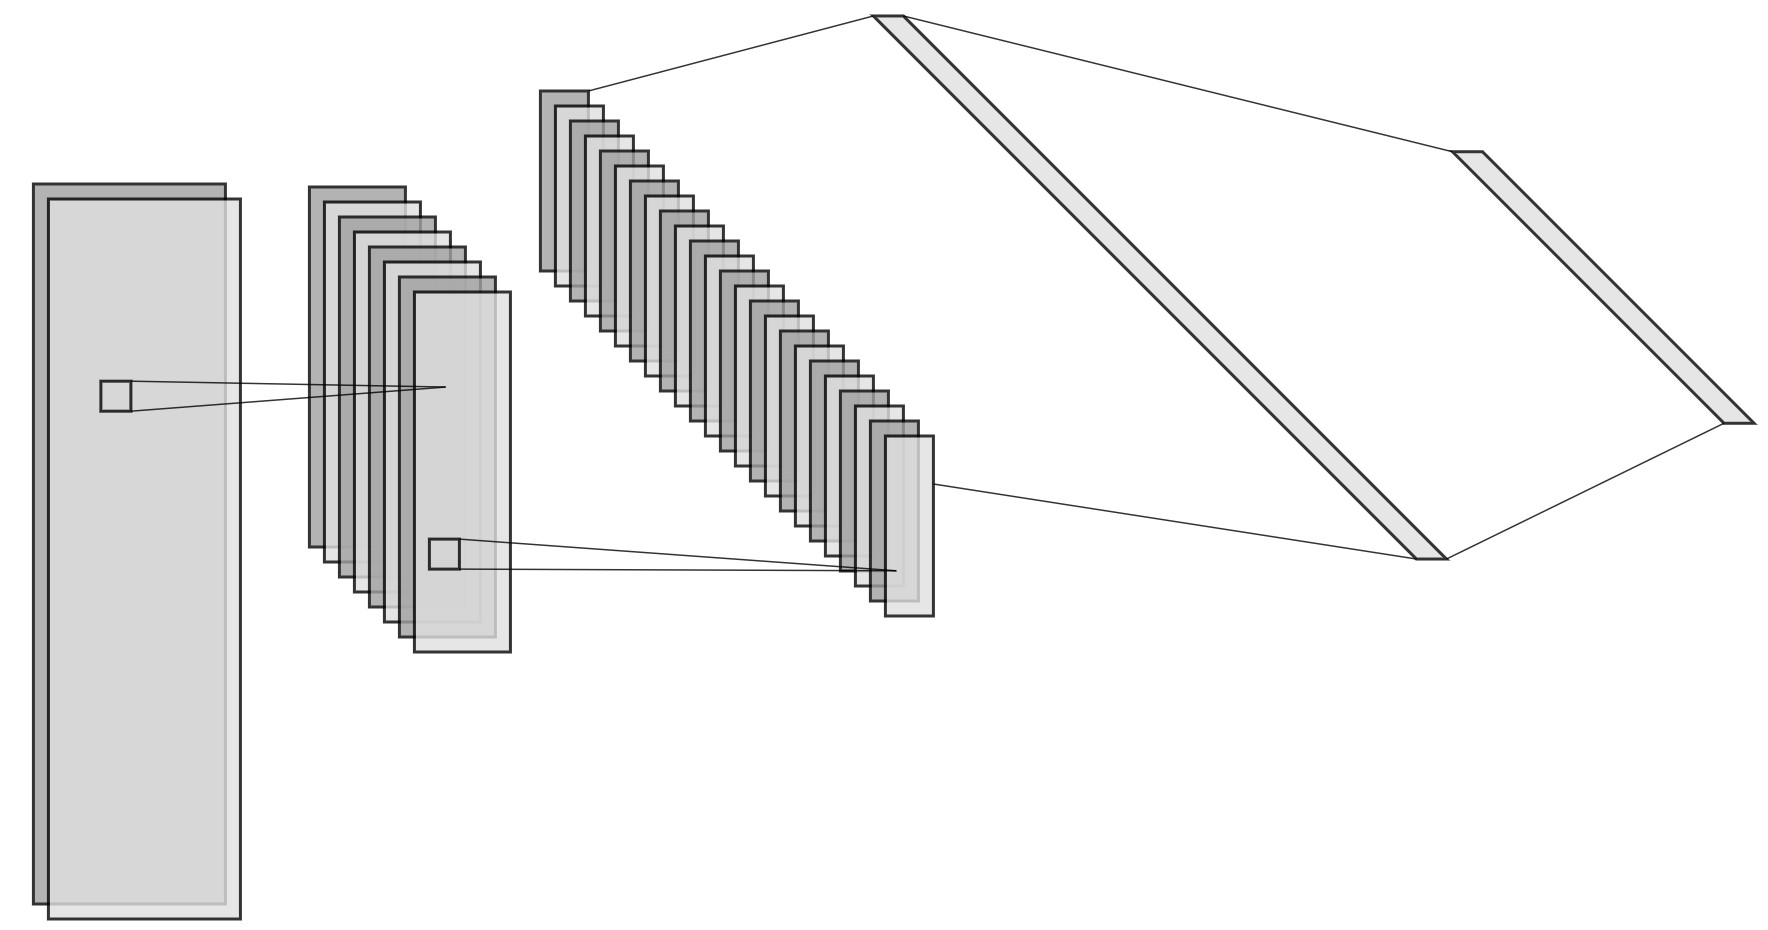
\includegraphics[width=0.8\textwidth]{images/nn/architectures/rmvae/encoder.jpg}
    \caption{RMVAE encoder architecture}
    \label{fig:rmvae_encoder}
\end{figure}

The filter sizes of the convolutional layers are \texttt{(5, 5)}.
I chose this dimension so the receptive field of the first layer is a third major interval and an entire beat.

\subsubsection{Recurrent encoder}
\label{sec:encoder:rnn}

For a given instrument $i$, and a given measure $m$, the tensor has a shape of \texttt{(16, 128, channels)}.
The first dimension ( \texttt{(16,)} ) corresponds of a sixteenth note (\musSixteenth) in time.
Therefore, I created an encoder using bidirectional LSTM cells.
This architecture is shown in the figure \ref{fig:lstm-encoder}.

\begin{figure}[htbp]
    \begin{center}
        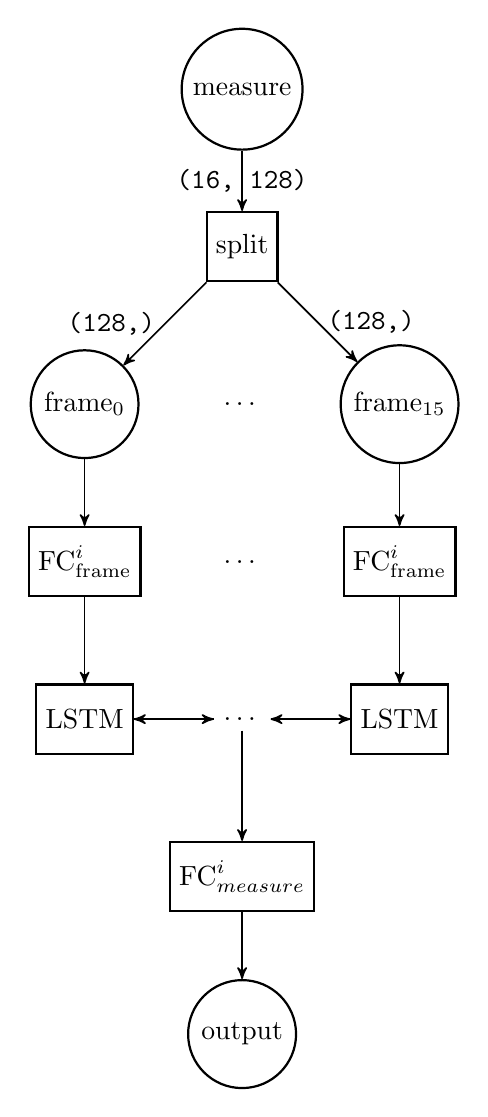
\begin{tikzpicture}[->, >=stealth', auto, semithick, node distance=2cm]
        \tikzstyle{every state}=[fill=white,draw=black,thick,text=black,scale=1]
        
        \node[state](measure)[]{measure};
        \node[state, rectangle](split)[below of=measure]{split};
        \node[](framedots)[below of=split]{$\dots$};
        \node[state](frame0)[left of=framedots]{$\text{frame}_0$};
        \node[state](frame15)[right of=framedots]{$\text{frame}_{15}$};
        
        \node[state, rectangle](fc0)[below of=frame0]{$\text{FC}_{\text{frame}}^i$};
        \node[](fcdots)[below of =framedots]{$\dots$};
        \node[state, rectangle](fc15)[below of=frame15]{$\text{FC}_{\text{frame}}^i$};
        
        \node[state, rectangle](lstm0)[below of=fc0]{LSTM};
        \node[](lstmdots)[below of=fcdots]{$\dots$};
        \node[state, rectangle](lstm15)[below of=fc15]{LSTM};
        
        \node[state, rectangle](fc)[below of=lstmdots]{$\text{FC}_{measure}^i$};
        
        \node[state](output)[below of=fc]{output};
        
        
        \path[]
            (measure)   edge    [anchor=center]node{\texttt{(16, 128)}}  (split)
            (split) edge    [anchor=east]node{\texttt{(128,)}}  (frame0)
                    edge    [anchor=west]node{\texttt{(128,)}}  (frame15)
            (frame0)    edge    node{}  (fc0)
            (frame15)   edge    node{}  (fc15)
            (fc0)   edge    node{}  (lstm0)
            (fc15)  edge    node{}  (lstm15)
            (lstm0) edge    node{}  (lstmdots)
            (lstmdots)  edge    node{}  (lstm0)
                        edge    node{}  (lstm15)
            (lstm15)    edge    node{}  (lstmdots)
            (lstmdots)  edge    node{}  (fc)
            (fc)    edge    node{}  (output);
                    
        \end{tikzpicture}
    \caption{Measure Encoder using bidirectional LSTM}
    Encoder for a measure of an instrument $i$. A measure has a shape of \texttt{(16, 128)} and a frame as a shape of \texttt{(128,)}.
    \label{fig:lstm-encoder}
    \end{center}
\end{figure}


\subsection{PoE}

For a given instrument $i$ and a given step $t$, the output of the encoder $\text{Enc}^i$ will then go through 2 different FC layers $\text{fc}^i_\mu$ and $\text{fc}^i_\sigma$ which will return the mean and variance of the encoded normal distribution (figure \ref{fig:rmvae_poe_fc}).

\begin{figure}[h]
    \centering
    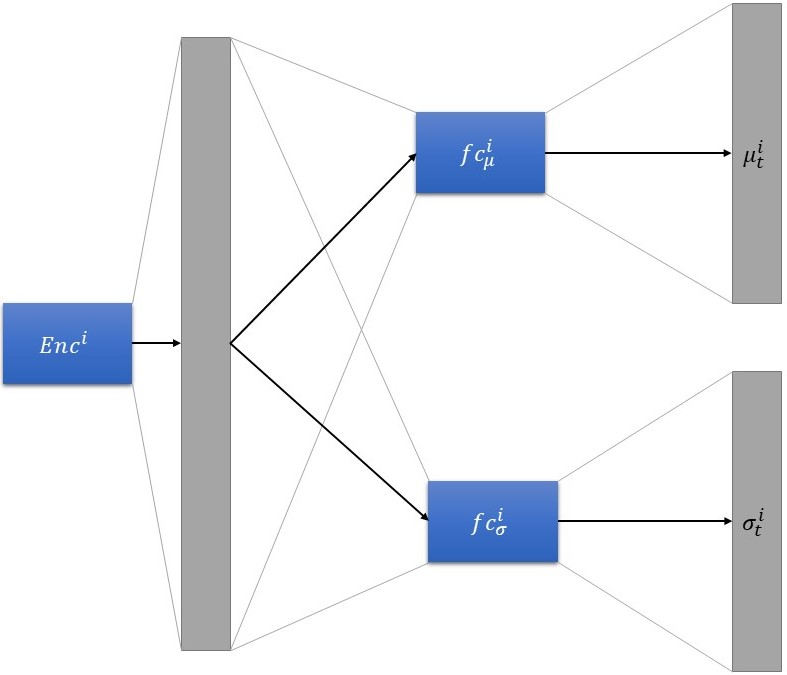
\includegraphics[width=0.6\textwidth]{images/nn/architectures/rmvae/poe_fc.jpg}
    \caption{RMVAE PoE Fully Connected layers}
    \label{fig:rmvae_poe_fc}
\end{figure}

Then, for a given step $t$, all the distribution representation go through the PoE layer to be combined and sampled as shown in the figure \ref{fig:mvae_architecture}.

\subsection{Recurrent layers}

I have now all the latent representations for every steps : $\{z_1, ..., z_T\}$.

\subsubsection{LSTM cells}

To learn, how this latent space evolves through time, RMVAE uses recurrent layers with LSTM cells (figures \ref{fig:rnn} , \ref{fig:lstm-gru}).
This is shown in the figure \ref{fig:rmvae_lstm}.


\begin{figure}
\begin{center}
    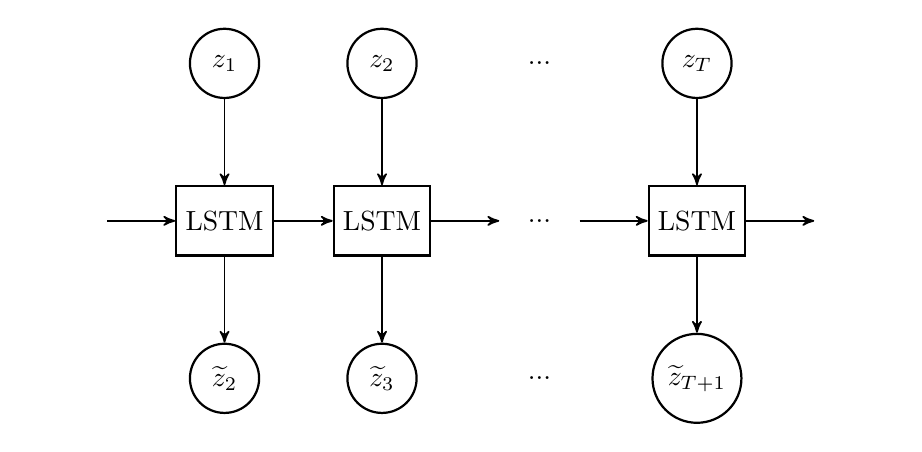
\begin{tikzpicture}[->, >=stealth', auto, semithick, node distance=2cm]
    \tikzstyle{every state}=[fill=white,draw=black,thick,text=black,scale=1]
    \node[state](z1)[]{$z_1$};
    \node[state](z2)[right of=z1]{$z_2$};
    \node[](dotsz)[right of=z2]{...};
    \node[state](zt)[right of=dotsz]{$z_T$};
    
    \node[state, rectangle](lstm1)[below of=z1]{$\text{LSTM}$};
    \node[state, rectangle](lstm2)[below of=z2]{$\text{LSTM}$};
    \node[minimum width=1cm](dotslstm)[below of=dotsz]{...};
    \node[state, rectangle](lstmt)[below
    of=zt]{$\text{LSTM}$};
    
    \node[state](zp2)[below of=lstm1]{$\widetilde{z}_2$};
    \node[state](zp3)[below of=lstm2]{$\widetilde{z}_3$};
    \node[](dotsz)[below of=dotslstm]{...};
    \node[state](zpt1)[below of=lstmt]{$\widetilde{z}_{T+1}$};
    
    \node[minimum width=1cm](whitelstmleft)[left of=lstm1]{};
    \node[minimum width=1cm](whitelstmright)[right of=lstmt]{};
    
    % -----
    
    \draw (z1) -> (lstm1);
    \draw (z2) -> (lstm2);
    \draw (zt) -> (lstmt);
    
    \draw (whitelstmleft) -> (lstm1);
    \draw (lstm1) -> (lstm2);
    \draw (lstm2) -> (dotslstm);
    \draw (dotslstm) -> (lstmt);
    \draw (lstmt) -> (whitelstmright);
    
    \draw (lstm1) -> (zp2);
    \draw (lstm2) -> (zp3);
    \draw (lstmt) -> (zpt1);
    
    \end{tikzpicture}
\end{center}
\caption{RMVAE LSTM layer}
\label{fig:rmvae_lstm}
\end{figure}

\subsubsection{RPoE}
\label{sec:rpoe}

To try to catch the time dependency as good as possible, I implemented a new layer architecture. I call it Recurrent Product of Experts (RPoE).

The result of the Product of Experts at the step $t$ is given as a modality for the Product of Experts at the step $t+1$.

The architecture is displayed in the figure \ref{fig:rpoe_architecture}.

\begin{figure}[h]
    \centering
    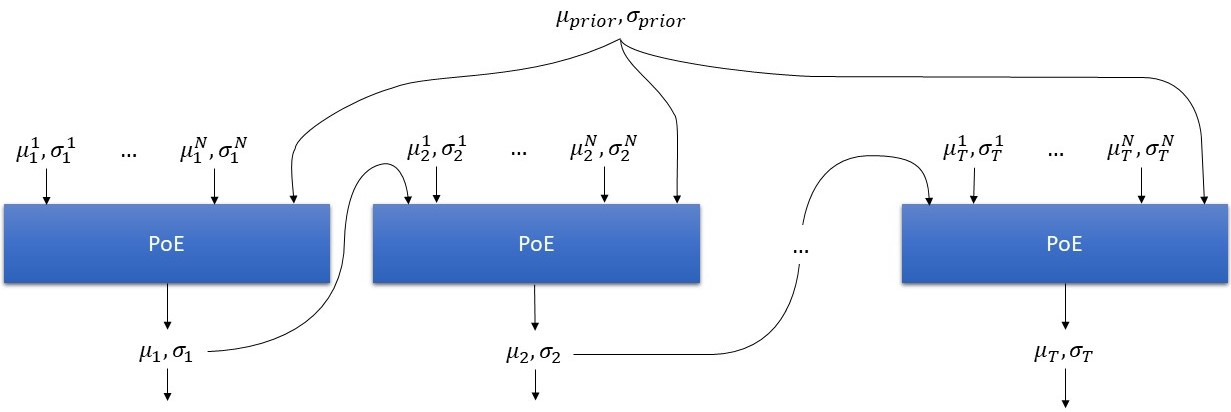
\includegraphics[width=\textwidth]{images/nn/architectures/rmvae/rpoe_architecture.jpg}
    \caption{RPoE architecture}
    \label{fig:rpoe_architecture}
\end{figure}


\subsection{Decoder}
\label{sec:decoder}

Each instruments (each modalities) has its own decoder.
The decoder $\text{Dec}^i$ associated to the instrument $i$ will, for a given step $t$, reconstruct back the output with the same shape as the input (\texttt{(16, 128, channels)}).

\subsubsection{Convolutional decoder}
\label{sec:decoder:cnn}

A decoder is composed of:
\begin{enumerate}
    \item Fully Connected layers
    \item Transposed Convolutional layers
\end{enumerate}
The dimensions of the layers of the encoder $\text{Enc}^i$ are the same as the dimensions of the decoder $\text{Dec}^i$.

The decoder global architecture is showed in the figure \ref{fig:rmvae_decoder}.

\begin{figure}[ht]
    \centering
    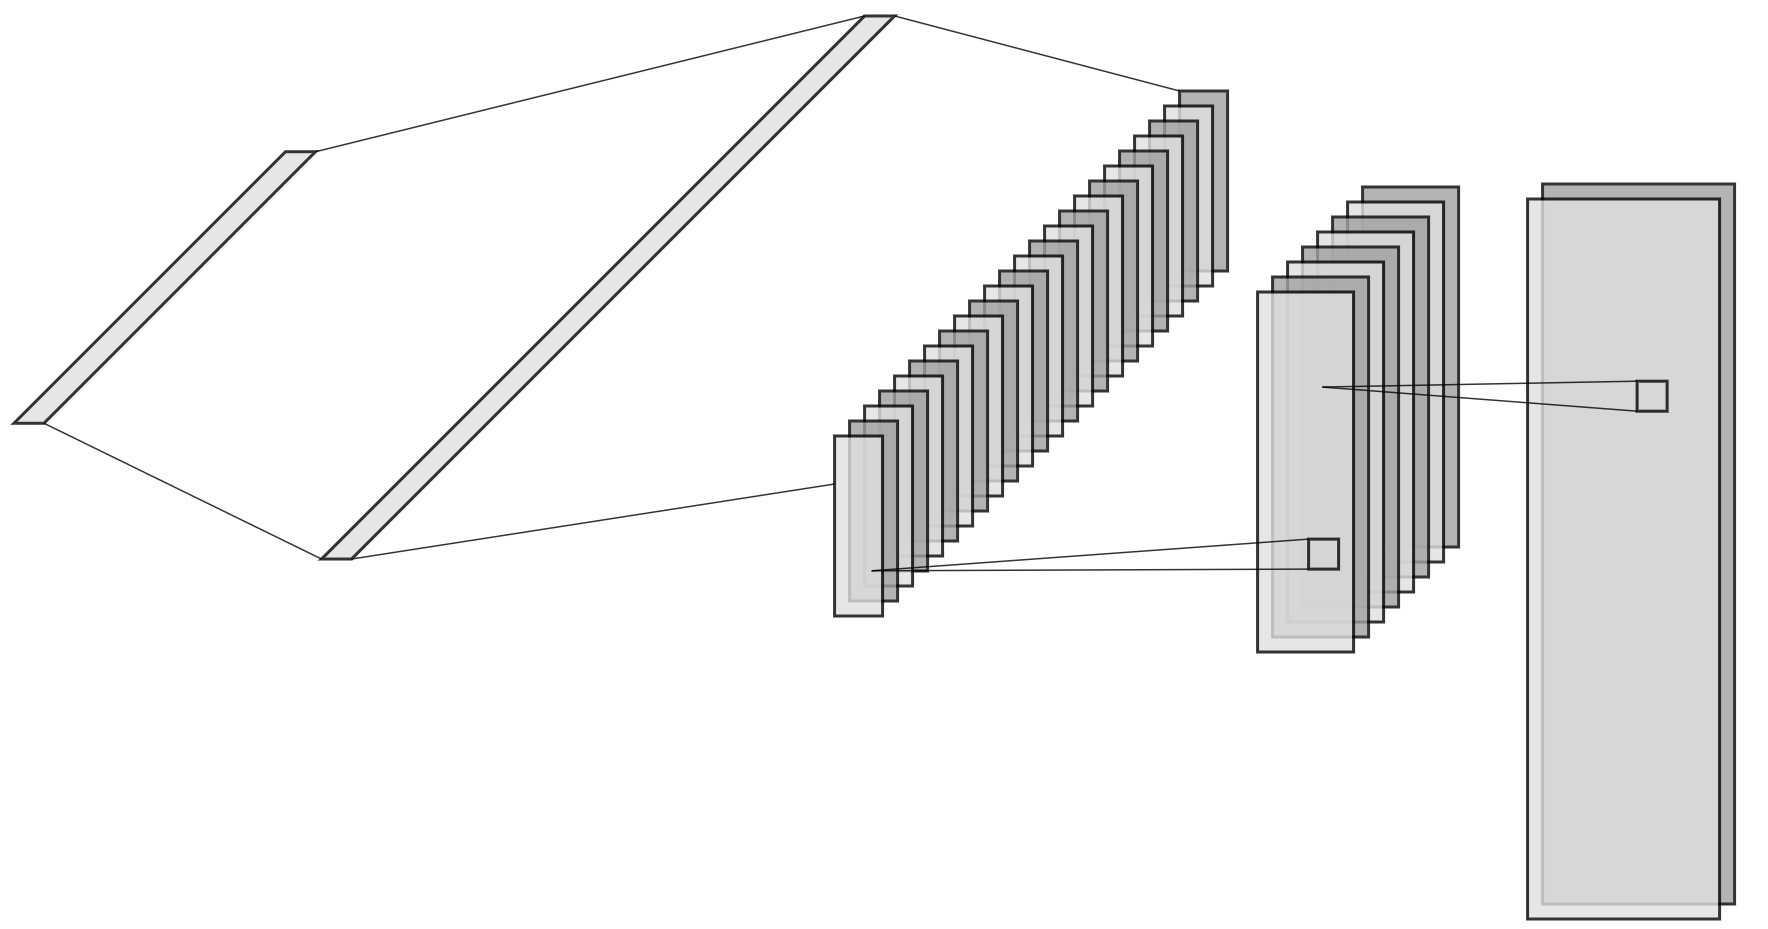
\includegraphics[width=\textwidth]{images/nn/architectures/rmvae/decoder.jpg}
    \caption{RMVAE decoder architecture}
    \label{fig:rmvae_decoder}
\end{figure}

This decoder was associated with the convolutional encoder from the section \ref{sec:encoder:cnn}.

\subsubsection{Recurrent decoder}
\label{sec:decoder:rnn}

To decode the latent space encoded with the recurrent encoder (from the section \ref{sec:encoder:rnn}), I use a recurrent architecture composed with bidirectional LSTM cells.
This architecture is illustrated in the figure \ref{fig:lstm-decoder}

\begin{figure}[H]
    \begin{center}
        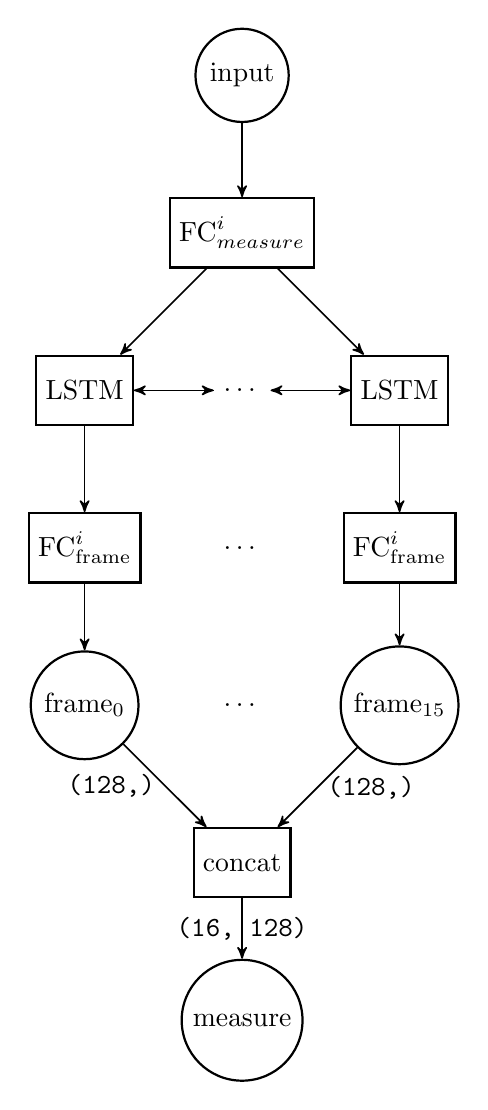
\begin{tikzpicture}[->, >=stealth', auto, semithick, node distance=2cm]
        \tikzstyle{every state}=[fill=white,draw=black,thick,text=black,scale=1]
        
        \node[state](measure)[]{measure};
        \node[state, rectangle](concat)[above of=measure]{concat};
        \node[](framedots)[above of=concat]{$\dots$};
        \node[state](frame0)[left of=framedots]{$\text{frame}_0$};
        \node[state](frame15)[right of=framedots]{$\text{frame}_{15}$};
        
        \node[state, rectangle](fc0)[above of=frame0]{$\text{FC}_{\text{frame}}^i$};
        \node[](fcdots)[above of =framedots]{$\dots$};
        \node[state, rectangle](fc15)[above of=frame15]{$\text{FC}_{\text{frame}}^i$};
        
        \node[state, rectangle](lstm0)[above of=fc0]{LSTM};
        \node[](lstmdots)[above of=fcdots]{$\dots$};
        \node[state, rectangle](lstm15)[above of=fc15]{LSTM};
        
        \node[state, rectangle](fc)[above of=lstmdots]{$\text{FC}_{measure}^i$};
        
        \node[state](input)[above of=fc]{input};
        
        
        \path[]
            (input) edge    node{}  (fc)
            (fc)    edge    node{}  (lstm0)
                    edge    node{}  (lstm15)
            (lstm0) edge    node{}  (fc0)
                    edge    node{}  (lstmdots)
            (lstmdots)  edge    node{}  (lstm0)
                        edge    node{}  (lstm15)
            (lstm15)    edge    node{}  (fc15)
                        edge    node{}  (lstmdots)
            (fc0)   edge    node{}  (frame0)
            (fc15)  edge    node{}  (frame15)
            (frame0)    edge    node[anchor=east]{\texttt{(128,)}}  (concat)
            (frame15)   edge    node[anchor=west]{\texttt{(128,)}}  (concat)
            (concat)    edge    node[anchor=center]{\texttt{(16, 128)}}  (measure);
                    
        \end{tikzpicture}
    \caption{Measure Decoder using bidirectional LSTM}
    Decoder for a measure of an instrument $i$. A measure has a shape of \texttt{(16, 128)} and a frame as a shape of \texttt{(128,)}.
    \label{fig:lstm-decoder}
    \end{center}
\end{figure}


\subsection{Last layer}

The last layer of the NN is a Fully Connected layer with a well chosen activation function.

\subsubsection{Polyphonic Music}

For polyphonic music (section \ref{sec:poly}), the activation function is a \textit{sigmoid} function for the \texttt{channel 1} which represents the activation of the notes.
The activation function for the \texttt{channel 2} is a \textit{ReLU} function.

\subsubsection{Monophonic Music}
\label{sec:last-layer-mono}

For monophonic music (section \ref{sec:mono}), the activation function is s \textit{sigmoid} function for the \textit{additional note} (index 128: $note_{continue}$) because it is an activation note indicating if it wants to continue the previous note or play a new one. And for the other 128 notes, the activation function is a \textit{softmax} function since only one note can be played at the same time.

At the beginning of my project, I was considering the $note_{continue}$ as a \textit{normal note} and I was simply applying a softmax activation across all the notes.
But the result was disappointing: the frequency of $note_{continue}$ in the dataset was to high.
The network wasn't generating anything because the $note_{continue}$ had the highest probability.

% -------------------- Loss Function --------------------

\section{Loss Function}
\label{sec:loss}

For this project, I created new loss functions to help the network to understand how music works.
As a musician, I asked myself how I would proceed if I was given the same task as the NN (generation of music, accompaniment...).
This is how I got the idea to create those new loss functions.

In a song, when a musician is playing, it is not possible for him play every one of the 12 notes whenever he wants.
A music usually follows a pattern, a chord progression, and the musician has to follows it.
From the chords played, the scale, some notes sounds better to the human ears than others.
But there is no \textit{"ground truth"} for a solo part for example.
Every solo can be considered as a \textit{"ground truth"} if it sounds nice.
I wanted my model to be able to \textit{improvise}, generate new music.

I got the idea of helping the model to do \textit{acceptable mistakes} and restraint it do to \textit{unacceptable mistakes}.
In other words, during the training part, if the model doesn't hit the note it should have hit, I don't want to \textit{punish} it to much with a high loss value if the note sounds actually nice with the music.
On the other side, I want to \textit{punish} it if the note it hits is completely wrong with a higher loss value.

To summarize what I previously just said, during the training part, if the model hits a note which sounds nice, a reward is given by adding a negative number to the loss.
If the hit note doesn't sound nice, then a penalty is given by adding a positive number to the loss.
The algorithm \ref{alg:loss} describes the process.

\begin{algorithm}
    \begin{algorithmic}[1]
        \Require{$noteTruth, notePredict$}
        \Ensure{$loss$}
        \Statex
        \State {$reward > 0, penalty >0$}
        \Function{Loss}{$noteTruth, notePredict$}
            \State {$loss \gets \texttt{commonLoss}(noteTruth, notePredict)$}
            \If{$\texttt{soundsGood}(notePredict)$}
                \State $loss \gets loss - reward$
            \Else
                \State $loss \gets loss + penalty$
            \EndIf
            \State \Return {$loss$}
        \EndFunction
    \end{algorithmic}
    \caption{Add a Reward or a penalty to the generated note}
    \label{alg:loss}
\end{algorithm}

The difficulty is to create the function \texttt{soundsGood} from the algorithm \ref{alg:loss}.
The following sections describe the idea I have had to know whether a note sounds nice or not.

\subsection{Scale}
\label{sec:scale}

I call this loss function \textit{Scale} because the idea is to reconstruct the \textit{local scale}.
This loss function takes as inputs all the instruments output:
\begin{center}
$\texttt{Scale}(truth, predict)$
\end{center}
where the shape of both input tensors is \texttt{(nb\_instruments, 16, 128)}.
It represents the activated notes (where there is a 1) of every instruments for the next measure.
The figure \ref{fig:loss_scale} shows the operations of this function.

The idea is to take all the played notes for all the instruments in the truth tensor.
Because the same note from different octaves should be considered as the same note, I apply a segment sum to get in the end a tensor of shape \texttt{(12,)} which corresponds to the 12 notes.
The details of the segment sum operation are explained in the appendix \ref{appendix:segment_sum}.
The result of this function will be positive for a note in the predict tensor which is not in the truth tensor.
Conversely, if the note in the predicted tensor is present in the truth tensor, the result will be negative.


\begin{figure}[h]
\begin{center}
    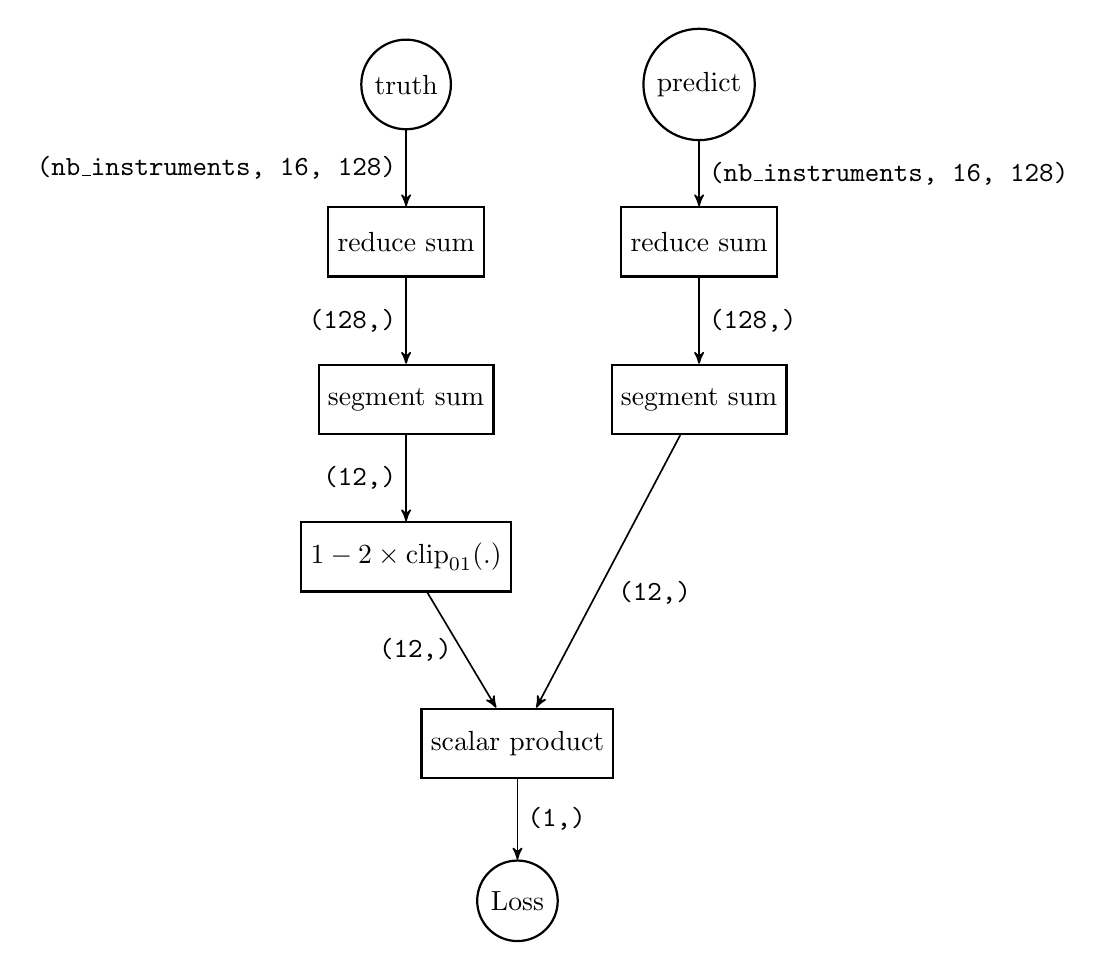
\begin{tikzpicture}[->, >=stealth', auto, semithick, node distance=2cm]
    \tikzstyle{every state}=[fill=white,draw=black,thick,text=black,scale=1]
    
    \node[state](truth)[left=1.cm]{ truth };
    \node[state](predict)[right of=truth, right=1.cm]{predict};
    
    \node[state, rectangle](t1)[below of=truth]{reduce sum};
    \node[state, rectangle](t2)[below of=t1]{segment sum};
    
    \node[state, rectangle](p1)[below of=predict]{reduce sum};
    \node[state, rectangle](p2)[below of=p1]{segment sum};
    
    \node[state, rectangle](t3)[below of=t2]{$1 - 2 \times \text{clip}_{01}(.)$};
    
    \node[state, rectangle](n1)[below right of=t3, below=0.5cm]{scalar product};
    
    \node[state](loss)[below of=n1]{Loss};
    
    
    \path[]
        (truth) edge    node[left]{\texttt{(nb\_instruments, 16, 128)}}   (t1)
        (t1)    edge    node[left]{\texttt{(128,)}}   (t2)
        
        (predict)   edge    node{\texttt{(nb\_instruments, 16, 128)}}   (p1)
        (p1)    edge    node{\texttt{(128,)}}   (p2)
        
        (t2)    edge    node[left]{\texttt{(12,)}}    (t3)
        (t3)    edge    node[left]{\texttt{(12,)}}    (n1)
        (p2)    edge    node{\texttt{(12,)}}    (n1)
        (n1)    edge    node{\texttt{(1,)}} (loss);
        
    \end{tikzpicture}
\end{center}
\caption{Scale Loss}
\label{fig:loss_scale}
\end{figure}

\subsection{Rhythm}
\label{sec:rhythm}

The idea behind the Rhythm loss is that we want to preserve the rhythm of the music.
Indeed, the rhythm is sometimes important and consistence is needed through the musical piece.
Thus, to preserve it, every time the model plays a note that is not played at the same time as an instrument in the ground truth, it gets a penalty.
Conversely, every time the model plays a note at the same time as another one in the ground truth, it gets a reward.

The implementation showed in the figure \ref{fig:loss_rhythm} is very similar to the Scale implementation.


\begin{figure}[h]
\begin{center}
    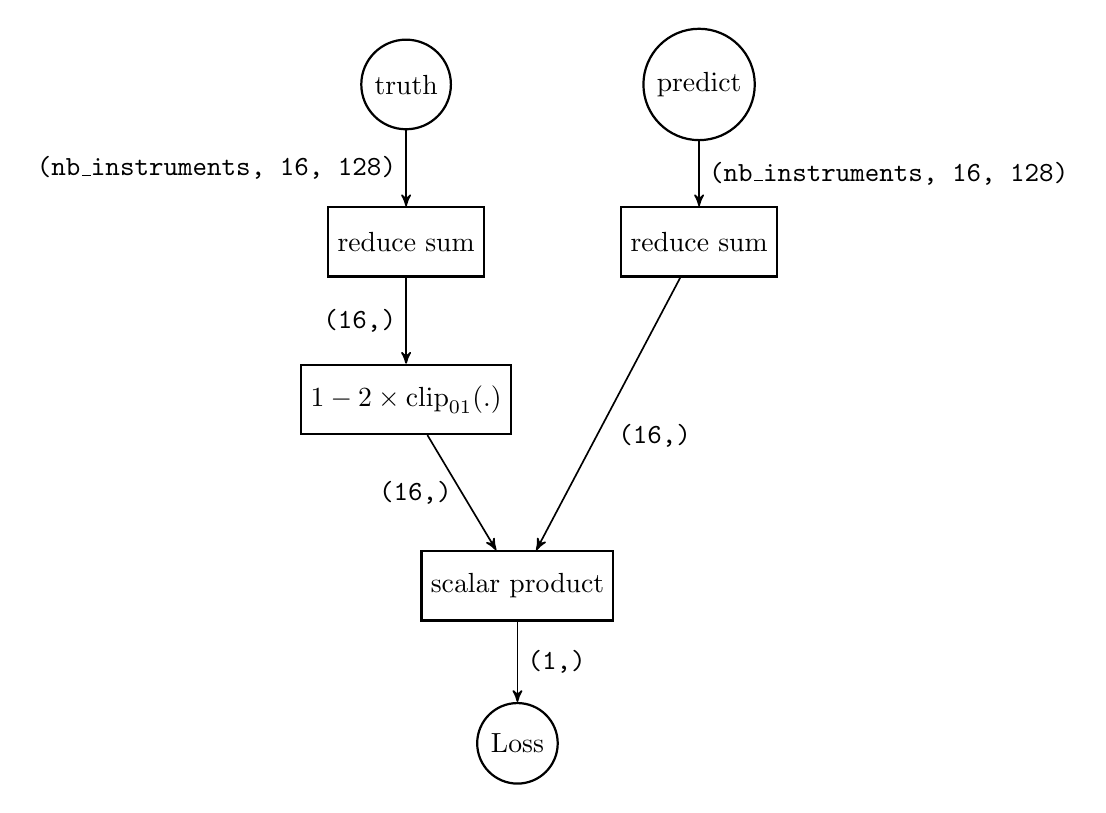
\begin{tikzpicture}[->, >=stealth', auto, semithick, node distance=2cm]
    \tikzstyle{every state}=[fill=white,draw=black,thick,text=black,scale=1]
    
    \node[state](truth)[left=1.cm]{ truth };
    \node[state](predict)[right of=truth, right=1.cm]{predict};
    
    \node[state, rectangle](t1)[below of=truth]{reduce sum};
    
    \node[state, rectangle](p1)[below of=predict]{reduce sum};
    
    \node[state, rectangle](t2)[below of=t1]{$1 - 2 \times \text{clip}_{01}(.)$};
    
    \node[state, rectangle](n1)[below right of=t2, below=0.5cm]{scalar product};
    
    \node[state](loss)[below of=n1]{Loss};
    
    
    \path[]
        (truth) edge    node[left]{\texttt{(nb\_instruments, 16, 128)}}   (t1)
        
        (predict)   edge    node{\texttt{(nb\_instruments, 16, 128)}}   (p1)
        
        (t1)    edge    node[left]{\texttt{(16,)}}    (t2)
        (t2)    edge    node[left]{\texttt{(16,)}}    (n1)
        (p1)    edge    node{\texttt{(16,)}}    (n1)
        (n1)    edge    node{\texttt{(1,)}} (loss);
        
    \end{tikzpicture}
\end{center}
\caption{Rhythm Loss}
\label{fig:loss_rhythm}
\end{figure}

\subsection{Harmony}
\label{sec:harmony}

I explained in the section \ref{sec:harmonics} that some notes will sound smooth together because of their common harmonics.
On the other side, some notes won't be elegant when played together because of the resonance problem between some of their harmonics.

This is something every composer has in mind when he creates a second musical part which will harmonize the first one.
He will keep the second voice in the scale and he will keep an acceptable musical interval between the notes of the 2 melodic parts.

The figure \ref{fig:harmony_circle} shows the \textit{acceptable} and \textit{non-acceptable} musical intervals for a $A$ note.

\begin{figure}[ht]
    \centering
    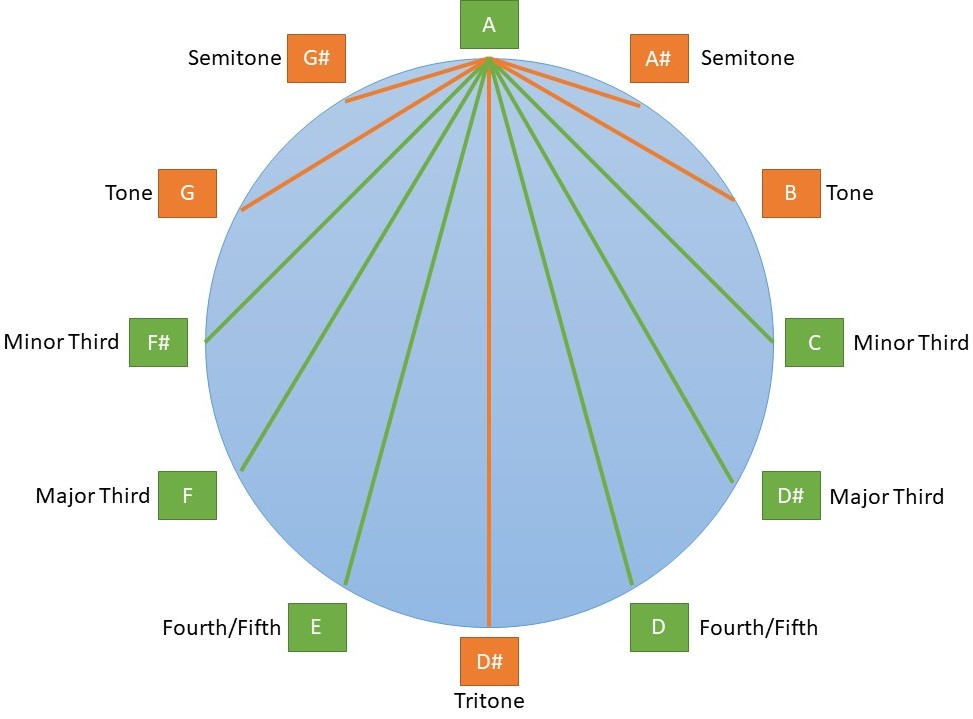
\includegraphics[width=\textwidth]{images/music/circle_harmony.jpg}
    \caption{Harmony Circle for $A$}
    \label{fig:harmony_circle}
\end{figure}

From this figure, I realized there are actually 3 musical intervals to avoid:
\begin{itemize}
    \item The \textit{semitone} interval
    \item The \textit{tone} interval
    \item The \textit{tritone} interval. This interval was named \textit{"Diabolus in musica"} ("Devil in the music") and was forbidden by the church.
\end{itemize}

To prevent the model to produce such intervals, I created a loss function which gives a penalty every time there is one of this intervals.
To do so, I created a sub-function $\text{harmony}_n$ which penalizes the presence of the $n^{th}$ interval (counted in semitone).

The operations of the cost function harmony and $\text{harmony}_n$ are showed in the figures \ref{fig:loss_harmony} and \ref{fig:loss_harmony_n}.
As for the Scale loss, the $\text{harmony}_{n}$ use a segment sum operation to get rid of the octaves.
The trick is to apply a $\text{roll}_{n}$ operation on the result and compute a scalar product with the original.
The $\text{roll}_n$ operation is explained in the appendix \ref{appendix:roll_n}.
It will return a positive and high value if an interval of $n$ semitones is present in the tensor.

The function Harmony do the sum of the functions $\text{harmony}_1$, $\text{harmony}_{2}$ and $\text{harmony}_{6}$ which respectively handle the semitone, tone, and tritone intervals.


\begin{figure}[htbp]
    \begin{minipage}{0.5\textwidth}
        \begin{center}
            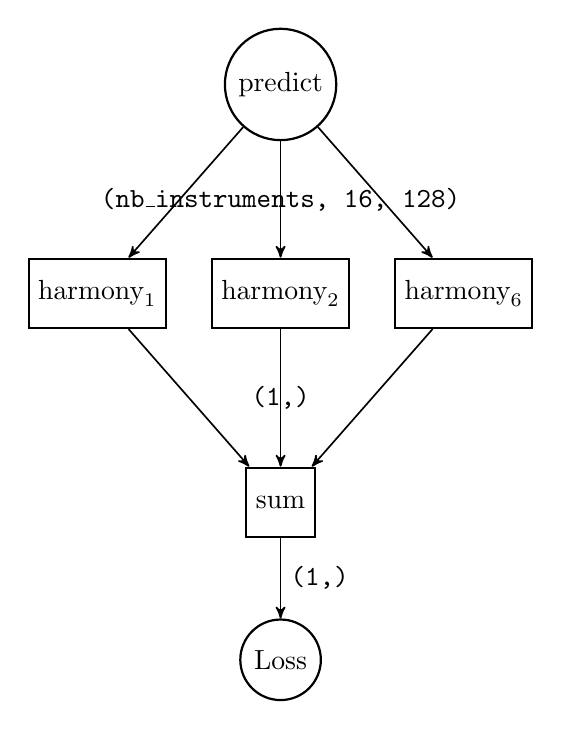
\begin{tikzpicture}[->, >=stealth', auto, semithick, node distance=2cm]
            \tikzstyle{every state}=[fill=white,draw=black,thick,text=black,scale=1]
            
            \node[state](n0)[]{predict};
            \node[](nleft)[left of=n0, left=0.2cm]{};
            \node[](nrigth)[right of=n0, right=0.2cm]{};
            
            
            \node[state, rectangle](h1)[below of=nleft, below=0.2cm]{$\text{harmony}_1$};
            \node[state, rectangle](h2)[below of=n0, below=0.2cm]{$\text{harmony}_2$};
            \node[state, rectangle](h6)[below of=nrigth, below=0.2cm]{$\text{harmony}_6$};
            
            \node[state, rectangle](s)[below of=h2, below=0.2cm]{sum};
            
            \node[state](loss)[below of=s]{Loss};
            
            \path[]
                (n0)    edge    node{}  (h1)
                        edge    node[anchor=center]{\texttt{(nb\_instruments, 16, 128)}}   (h2)
                        edge    node{}  (h6)
                (h1)    edge    node{}  (s)
                (h2)    edge    node[anchor=center]{\texttt{(1,)}}  (s)
                (h6)    edge    node{}  (s)
                (s)     edge    node{\texttt{(1,)}} (loss);
                
            \end{tikzpicture}
        \end{center}
        \caption{Harmony Loss}
        \label{fig:loss_harmony}
    \end{minipage} \hfill
    \begin{minipage}{0.5\textwidth}
        \begin{center}
            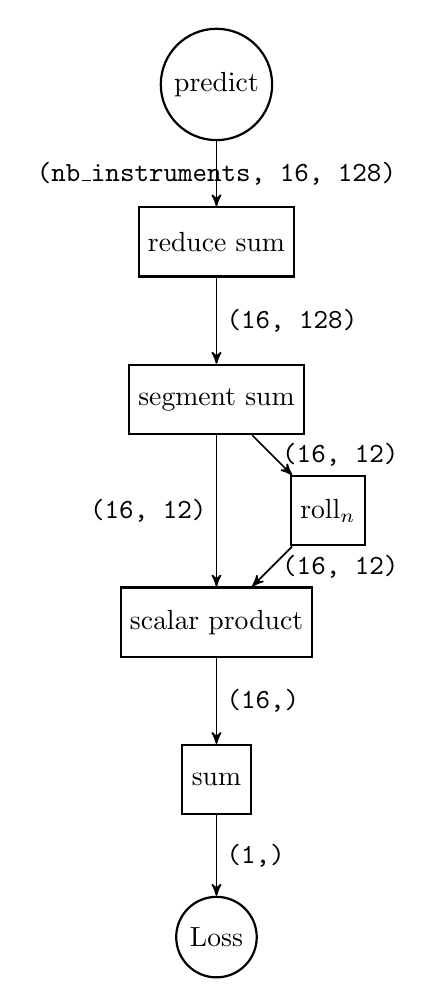
\begin{tikzpicture}[->, >=stealth', auto, semithick, node distance=2cm]
            \tikzstyle{every state}=[fill=white,draw=black,thick,text=black,scale=1]
            
            \node[state](predict)[]{predict};
            
            \node[state, rectangle](n1)[below of=predict]{reduce sum};
            \node[state, rectangle](n2)[below of=n1]{segment sum};
            
            \node[state, rectangle](r)[below right of=n2]{$\text{roll}_n$};
            
            \node[state, rectangle](s)[below left of=r]{scalar product};
            
            \node[state, rectangle](sum)[below of=s]{sum};
            
            \node[state](loss)[below of=sum]{Loss};
            
            
            \path[]
                (predict)   edge    node[anchor=center]{\texttt{(nb\_instruments, 16, 128)}}    (n1)
                (n1)    edge    node{\texttt{(16, 128)}}   (n2)
                (n2)    edge    node[right]{\texttt{(16, 12)}}    (r)
                        edge    node[left]{\texttt{(16, 12)}}  (s)
                (r)     edge    node[right]{\texttt{(16, 12)}} (s)
                (s)     edge    node{\texttt{(16,)}} (sum)
                (sum)     edge    node{\texttt{(1,)}} (loss);
                
            \end{tikzpicture}
        \end{center}
        \caption{$\text{Harmony}_n$ Loss}
        \label{fig:loss_harmony_n}
    \end{minipage}
\end{figure}

\section{Learning process}
\label{sec:learning-process}

% TODO: training : prediction
% DONE

In this section I will describe how I train the Recurrent Multimodal Variational AutoEncoder.
I use the model differently between the training time and the creation time.

During the training, the model is trained to predict the next measure of a song from a fixed number of measures.
In practice, I give 8 measures of a song from the Bach Chorale corpus and ask the model to predict the next one.
The goal is not to \textit{over fit} the training dataset.
During the training time, the model will try to \textit{guess} and learn what is the next measure from the previous ones for the songs in the dataset.
The idea is that the model will not learn all the songs \textit{by heart}, but it will learn music in a more general and meaningful way.
It will learn musical rules, tendencies, and styles from the dataset.

Then, when the model is correctly trained, it will be able to complete a song in a consistent way from the given seed and the train dataset.
When 8 measures from the test dataset are given to the model, it will create the next measure which can be a possible continuation of the given seed.
Obviously the model won't be able to guess and recreate the correct measure from the song because it is impossible to \textit{guess} a song without hearing it before.
So the model will create an alternative continuation of a song and this is how it can be used to create a new song.

Alternatively, the seed given to the model can be random so the RMVAE will generate new measures on its own. 


% ----------------------------------------------------------------------------------------------------
% Results
% ----------------------------------------------------------------------------------------------------
\chapter{Results}
\label{chap:results}

In this chapter I will share the results I got.
In the section \ref{sec:results:evaluation}, I will explained how I decided to evaluate the music samples created by my model.
In the section \ref{sec:results:samples}, I will describe what sample the model usually produces.
In the section \ref{sec:results:note-continue}, I will show the results obtained when the model is using or not the $\text{note}_{\text{continue}}$ note.
Finally, in the section \ref{sec:tasks}, I will enumerate what tasks I have actually implemented.
To be fair, the results are quite poor and disappointing.

% -------------------- Generated samples --------------------

\section{Music evaluation}
\label{sec:results:evaluation}

% TODO: Explain how to evaluate the music

Music is by definition an art, it is therefore subjective.
There is no way to measure the \textit{goodness} of a song.
Some people can like a music while others won't consider it is not enjoyable.
A way to rank songs is to look at how famous they are.
The most famous songs are the ones liked by more, therefore they must be good ?
This is not wrong but I am sure everyone reading this sentence can come with multiple famous songs they really don't like and multiple unknown songs they consider as outstanding...
It is possible to extract some rules, trends or recurrent patterns from music and this is what I have been trying to do during my all project.

However musicians always try to break these rules in different elegant ways to add some variation, originality and keep their songs interesting.
Consequently, every time I was identifying a trend, I was then facing a huge number of counter example to invalidate my thinking.
These counter examples can be encountered for different reasons:
\begin{itemize}
    \item The style of music is different.
    Classical, jazz or pop musics don't have the same rules and trends within each other.
    \item The instrument is different.
    A guitar musical line and an organ musical line are different.
    These differences comes from 2 factors.
    The first one is because of the way the instruments are played by the player.
    A guitar gives access of only 6 strings to the guitarist and the organ provides several keyboards to the organist.
    The sound also is important, the harmonics, the sustain, attack, release of a instrument impact how it is played.
    As a comparison, harpsichord, piano and organ songs are very different whereas the players have access to a keyboard to play.
    \item The player or composer is different.
    Different people will have different opinion and preferences about how their music should be.
\end{itemize}

\subsection{Prediction evaluation}

During the training time, the model performs a prediction task, the objective is to reconstruct the next measure from the previous ones given as in input.
Therefore, several metrics can be used to evaluate the performance of the neural network.
I will enumerate here the metrics I have been using to evaluate a train.
The objective is to reach the best value of the following metrics on the train and validation dataset (mostly validation data).

\subsubsection{Loss Function}

The loss function is a categorical cross-entropy loss function from a softmax activation (equations \ref{eq:ce} and \ref{eq:softmax}).
The goal is to obtain a loss as low as possible because this is an error function.

\begin{equation}
    CE = - \sum_{c=1}^{C} y_{truth} \log(y_{predict})
    \label{eq:ce}
\end{equation}
\begin{equation}
    \text{Softmax}(x)_{i} = \frac{e^{x_i}}{\sum_{c=1}^{C} e^{x_{c}}}
    \label{eq:softmax}
\end{equation}

However, two facts don't allow us to be able to generalize and rely to much on this loss value.
\begin{enumerate}
    \item This value is \textit{directly} minimized by the gradient descent algorithm.
    Therefore, the value has no choice but decrease through time.
    \item This value is artificial and is not musically meaningful.
    I have constructed this loss from a computer student's point of view.
    There is no direct link with music quality.
\end{enumerate}

\subsubsection{Accuracy metric}

The accuracy between the output of the model and the actual next measure of song can be calculated.
The accuracy represents the proportion of notes the model correctly predicts (including the note $\text{note}_{\text{continue}}$).
The algorithm \ref{alg:accuracy} describes how the accuracy is calculated.
The objective is to inscrease the accuracy as much as possible.

\begin{algorithm}
    \begin{algorithmic}[1]
        \Require{$truth$ (tensor of shape \texttt{(16, 128 + 1)}), $predict$ (tensor of shape \texttt{(16, 128 + 1)})} 
        \Ensure{$acc$}
        \Statex
        \Function{accuracy}{$truth$, $predict$}
            \State $truthArgs \gets argmax(truth, axis=1)$ \texttt{// (16,)}
            \State $predictArgs \gets argmax(predict, axis=1)$ \texttt{// (16,)}
            \State $acc = 0$
            \For{$k \gets 0$ to $15$}
                \If{$truthArgs[k] == predictArgs[k]$}
                    \State $acc \gets acc + 1$
                \EndIf
            \EndFor
            \State $acc \gets acc / 16$
            \State \Return {$acc$}
        \EndFunction
        \end{algorithmic}
    \caption{Accuracy function}
    \label{alg:accuracy}
\end{algorithm}

This accuracy is more meaningful than the loss because it is not directly minimized by the gradient descent algorithm.
However, it is still strongly linked to the loss value by the way it is constructed.
As the loss value, the accuracy is not musically meaningful.

For example, in the figure \ref{fig:acc-difference}, let us say the first measure is the target measure, and the measures 2 and 3 are 2 measures created by 2 different models.
\begin{itemize}
    \item  The measures 1 and 2 are musically similar: both of them are a arpeggio of the $G$ major chord and the accuracy computed would be $0.5$.
    \item The measures 1 and 3 are not musically alike, the measure 3 contains a melody which is not in $G$ major.
    However, the accuracy computed would be $0.75$.
\end{itemize}
The first model would be the best for a musician but for a computer student or an gird search algorithm, the second model would be the preferred one.

\begin{figure}[htbp]
    \centering
    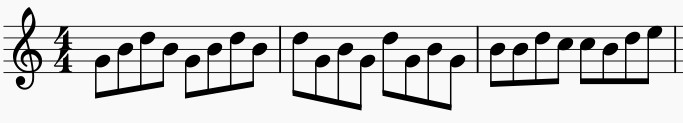
\includegraphics[width=\textwidth]{images/metrics/training/acc.jpg}
    \caption{musical measure examples}
    \label{fig:acc-difference}
\end{figure}

\subsubsection{KLD}

The KLD is a cost function applied on the latent space of the VAE, MVAE and RMVAE.
The goal is to have a KLD as low as possible.
The lower the KLD value is, the higher are the chances the model is not overfitting and generalizing in a meaningful the data it is feed with.
However, this value is directly minimized by the gradient descent and has no link with musical quality.

\subsubsection{Custom loss functions}
\label{sec:evaluate:train:custom-loss}

The custom loss functions I have created for this project (Scale, Rhythm and Harmony) can be used as metric to evaluate a model.
For all of them, the objective is to have a value as low as possible.
However there are several issues with these values:
\begin{itemize}
    \item The values of the loss functions are directly minimized by the gradient descent algorithm.
    The values are forced to decreased and a low value won't necessarily imply a successful train.
    \item I have constructed these values from my understanding and music.
    As said previously, there is no fixed rules in music, and the logic behind these functions can sometimes goes against a song philosophy.
\end{itemize}

\subsection{Creation evaluation}

After the training, the trained model has learnt a representation about music and generalized it in its own way.
As explained in the section \ref{sec:learning-process}, the model will either generate a song or complete one in a consistent way.
During this creation process, there is no ground truth to compare the generation with as during the training time.
As I said previously, the model is expected to \textit{create a new song} with new musical part as it was performing a solo or composing music.
And every solo can be considered as \textit{correct} as long as it sounds nice to us, which is very subjective.

However for this project, I need to evaluate the created musical parts by my different models.
To do so, I can look at the harmony loss value I created (section \ref{sec:harmony}).
And the most common process to evaluate music through the related works about music is to ask the public.
Some surveys are organized, and people are answering them to vote for the best produced sample.

\subsubsection{Harmony loss function}
\label{sec:eval:creation:harmony}

The harmony loss function I have created in the section \ref{sec:harmony}, is a cost function which takes as an input only the created tensor.
It doesn't need the truth tensor from the training, therefore I can evaluate its value with a created sample.

However, as explained previously in the section \ref{sec:evaluate:train:custom-loss}, the harmony value is directly minimized by the gradient descent and a low value doesn't necessarily mean the produced music is satisfactory.

Unfortunately, after several creation of music sample in the section \ref{sec:tasks} and some comparisons between different models in the chapter \ref{chap:experiments}, it appears the value of the harmony loss function doesn't add any understanding to the quality to the music...
The harmony value between a seed and the completed part (explained in the section \ref{sec:tasks:generate}) is not actually different.

Therefore, I won't use it to evaluate created sample in this report and I will only mention it when I consider it pertinent.

Moreover, \textit{real music} doesn't have an harmony value of $0$ because the compositors and players like to put some \textit{tension} in their songs.
That is another reason to not focus too long on the harmony value, a low value doesn't imply it is a good song.

\subsubsection{Public opinion}
\label{sec:eval:creation:public}

The strongest evaluation for music is the general opinion.
Despite the existence of some musical rules, judging and evaluating a musical piece is a subjective task.
Most of the papers working on music use the population to evaluate whether their model is qualitative enough. \cite{huang_counterpoint_2017, hadjeres_deepbach:_2016, huang_music_2018, liang_automatic_2017, huang_bach_2019}.
They create a poll and let the people decide what sample they prefer between several of them.

By lack of time and result, I haven't been able to create many polls to evaluate the musical samples my model creates.
The appendix \ref{appendix:google-forms} contains the list of all the different polls I have made for this Dissertation.

\section{Created Samples}
\label{sec:results:samples}

\subsection{CNN Encoder Decoder}

For a CNN encoder and decoder, the results weren't matching my expectation.
To illustrate it with an image, the figure \ref{fig:rmvae-generated} shows a completed sample by a RMVAE.

\begin{figure}[htpb]
    \centering
    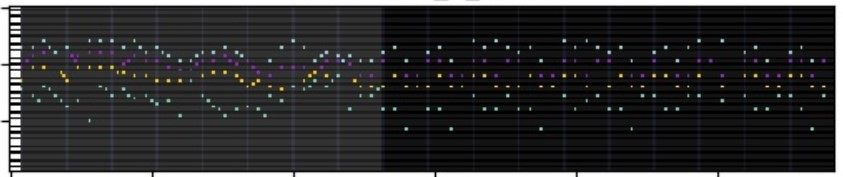
\includegraphics[width=\textwidth]{images/generated_midis/RMVAE/generated_cnn.jpg}
    \caption{Created pianoroll by the RMVAE with CNN encoder decoder}
    The grey part is the seed given to the model and the black part is the created part   (\href{https://github.com/ValentinVignal/midiGenerator/blob/master/samples/results/generated_pianoroll.mid}{Link})
    \label{fig:rmvae-generated}
\end{figure}

As we can see on the figure \ref{fig:rmvae-generated}, the global shape of the the created part is very different from the seed part.
The main reason is a lack of rhythm and variation.
Most of the created notes are quarter notes (\musQuarter), and the model produces always the same notes.

However, even though the created sample have huge lack of rhythm and variation, it is not wrong.
It is on tune, consistent with the seed, and the four voices work well together.

\subsection{Recurrent Encoder Decoder}

For the recurrent encoder and decoder, the results have been slightly better but not much.
The created samples are mostly composed of quarter notes (\musQuarter) and the variations are too poor.
One sample is showed in the figure \ref{fig:rrmvae-generated}.
The generated sample seems more complex with more variations.
And this is verified when you listen to it.
There are more small variations in the rhythm and the played note than the sample from the cnn encoder decoder.

\begin{figure}[htpb]
    \centering
    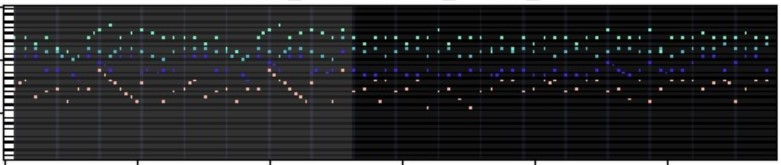
\includegraphics[width=\textwidth]{images/generated_midis/RRMVAE/generated-rnn.jpg}
    \caption{Created pianoroll by the RMVAE with recurrent encoder decoder}
    The grey part is the seed given to the model and the black part is the created part   (\href{https://github.com/ValentinVignal/midiGenerator/blob/master/samples/results/generated-pianoroll-rnn.mid}{Link})
    \label{fig:rrmvae-generated}
\end{figure}


% -------------------- Activation function --------------------


\section{Activation function of the $\text{note}_{\text{continue}}$ for monophonic music}
\label{sec:results:note-continue}

\subsection{CNN Encoder Decoder}

As explained in the section \ref{sec:last-layer-mono}, for monophonic music, I consider an extra note ($note_{continue}$) which indicates that the previous note is sustained.
The shape for a tensor describing a measure is \texttt{(16, 128 + 1)}.

At the beginning, I considered the $note_{continue}$ as a \textit{normal} note, and apply a softmax activation through the \texttt{128 + 1} notes for each of the 16 frames.
Unfortunately, it resulted with a too high probability for the $note_{continue}$ and the model wasn't generated anything.
The figure \ref{fig:rmvae-generated-silence} shows a created sample.
As explained, the produced part (black part) contains only few notes.

\begin{figure}[htbp]
    \centering
    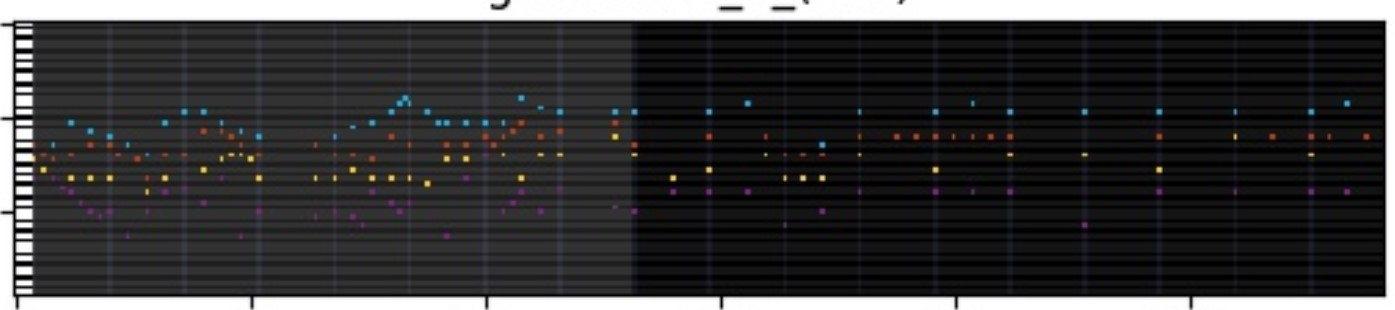
\includegraphics[width=\textwidth]{images/generated_midis/RMVAE/cnn_generation_silence.jpg}
    \caption{Created pianoroll by the RMVAE with a softmax activation}
    The grey part is the seed given to the model and the black part is the created part
    (\href{https://github.com/ValentinVignal/midiGenerator/blob/master/samples/results/generated_silence.mid}{Link})
    \label{fig:rmvae-generated-silence}
\end{figure}

To counter this silence problem I changed the activation function of the notes:
\begin{itemize}
    \item The $note_{continue}$ activation is a sigmoid activation.
    If the value is $\geq 0.5$, then no new note is played and the previous note is sustained.
    If the value is $< 0.5$, then a new note is played
    \item The \texttt{128} remaining notes are still going through a softmax activation to chose what is the note to be played (if $note_{continue} <0.5$).
\end{itemize}

By doing so, I helped the model to produce new notes and get results like the figure \ref{fig:rmvae-generated}.
However, the lack of rhythm is still present and most of the notes have a length of one beat (\musQuarter).


\subsection{LSTM Encoder and Decoder}

With the recurrent architecture (explained in sections \ref{sec:encoder:rnn} and \ref{sec:decoder:rnn}), I obtained the same behavior as with convolutional architecture (sections \ref{sec:encoder:cnn} and \ref{sec:decoder:cnn}).

The figures \ref{fig:pianoroll:rrmvae:no-binary} and \ref{fig:pianoroll:rrmvae:with-binary} illustrate it.
We can see on the pianoroll views that the created music is more consistent when the activation function on the note $note_{continue}$ is the sigmoid function.

\begin{figure}[htbp]
    \centering
    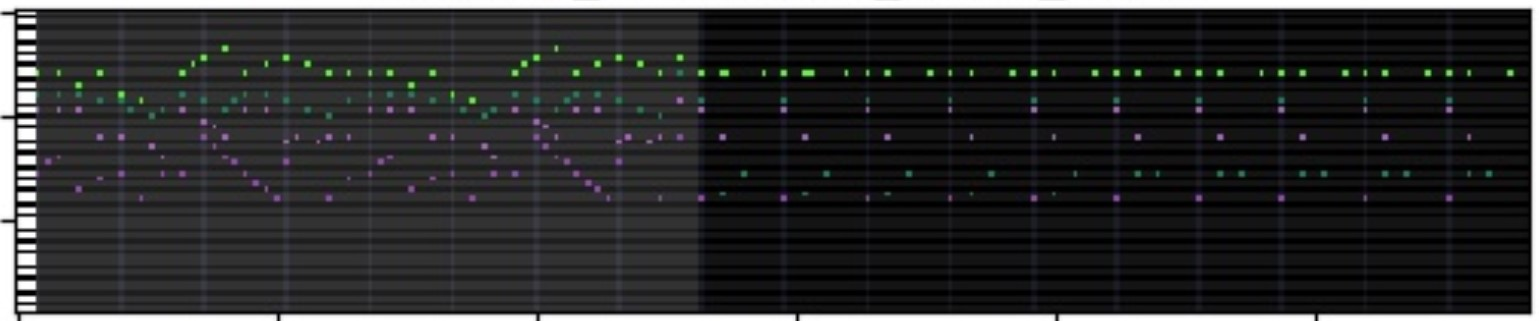
\includegraphics[width=\textwidth]{images/generated_midis/RRMVAE/pianoroll-rrmvae-no-binary.jpg}
    \caption{Created pianoroll by the RMVAE with recurrent architecture with softmax activation}
    The grey part is the seed given to the model and the black part is the created part
    (\href{https://github.com/ValentinVignal/midiGenerator/blob/master/samples/results/lstm_encoder_decoder.mid}{Link})
    \label{fig:pianoroll:rrmvae:no-binary}
\end{figure}

\begin{figure}[htbp]
    \centering
    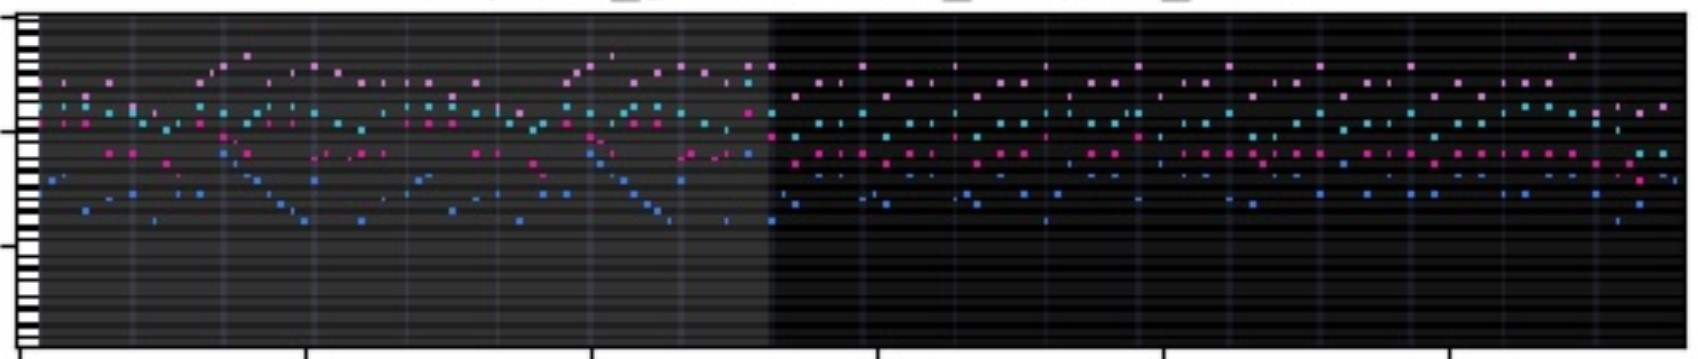
\includegraphics[width=\textwidth]{images/generated_midis/RRMVAE/pianoroll-rrmvae-with-binary.jpg}
    \caption{Created pianoroll by the RMVAE with recurrent architecture with softmax and sigmoid activation}
    The grey part is the seed given to the model and the black part is the created part
    (\href{https://github.com/ValentinVignal/midiGenerator/blob/master/samples/results/rrmvae-with-binary.mid}{Link})
    \label{fig:pianoroll:rrmvae:with-binary}
\end{figure}

However, the issues stay the same.
There is absolutely no rhythm, all the notes are quarter notes (\musQuarter) and there is no variation.
For instance, in the figure \ref{fig:pianoroll:rrmvae:with-binary}, the first voice (the pink one at the top) is only playing 3 different notes.

\section{Tasks}
\label{sec:tasks}

I created several scripts to use a single trained model for several tasks.
Those tasks are:
\begin{itemize}
    \item Complete (section \ref{sec:tasks:generate})
    \item Fill (section \ref{sec:tasks:fill})
    \item Redo (section \ref{sec:tasks:redo})
    \item Generate (section \ref{sec:tasks:generate-noise})
\end{itemize}


\subsection{Complete}
\label{sec:tasks:generate}

This is the simplest task I have created for the model.
The figure \ref{fig:tasks:generate} is the result of it.

\begin{figure}[htbp]
    \centering
    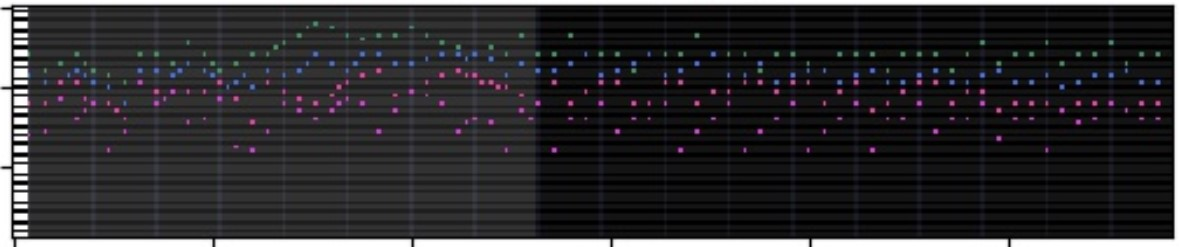
\includegraphics[width=\textwidth]{images/generated_midis/tasks/generate/generate.jpg}
    \caption{Task \textit{Complete}}
    (\href{https://github.com/ValentinVignal/midiGenerator/blob/master/samples/tasks/generate.mid}{Link})
    \label{fig:tasks:generate}
\end{figure}

The model is given a seed (grey part of the figure \ref{fig:tasks:generate}).
From this seed it creates the next measure.
It will then consider the seed and the previously created measure to create the next one.
And so one...

The algorithm \ref{alg:tasks:generate} describes this task.

\begin{algorithm}
    \begin{algorithmic}[1]
        \Require{$seed$ (list of measures), $n$ (number of generated measures)} 
        \Ensure{$generation$ (list of measures)}
        \Statex
        \Function{complete}{$seed$, $n$}
            \State $seed\_length \gets len(seed)$
            \State $generation \gets seed$
            \For{$k \gets 1$ to $n$}
                \State $input \gets generation[-seed\_length:]$
                \State $output \gets model.predict(input)$
                \State $generation.append(output)$
            \EndFor
            \State \Return {$generation$}
        \EndFunction
        \end{algorithmic}
    \caption{Complete function}
    \label{alg:tasks:generate}
\end{algorithm}

The RMVAE takes a mask as an input with a shape of \texttt{(nb\_instruments, nb\_measure)}.
Therefore, to ignore one or several instrument(s), the only thing to do is to put $0$ at the positions $mask[i, :]$ for every instrument $i$ we want to ignore.

However, as you can see in the figures \ref{fig:tasks:generate}, the created sample is poor in variation and complexity.
The accuracy of the model to create the next measure is around $0.8$, the harmony loss value of the  

\subsection{Fill}
\label{sec:tasks:fill}

The \textit{Fill} task creates a musical part (an instrument voice) from the others.
As an example, the figures \ref{fig:tasks:fill:truth} and \ref{fig:tasks:fill:0} illustrate this task.

\begin{figure}[htbp]
    \centering
    \includegraphics[width=\textwidth]{images/generated_midis/tasks/fill/task-fill-truth.jpg}
    \caption{Song given to the model for the \textit{Fill} task}
    (\href{https://github.com/ValentinVignal/midiGenerator/blob/master/samples/tasks/fill_truth.mid}{Link})
    \label{fig:tasks:fill:truth}
\end{figure}

\begin{figure}[htbp]
    \centering
    \includegraphics[width=\textwidth]{images/generated_midis/tasks/fill/task-fill-0.jpg}
    \caption{Output of the model for the \textit{Fill} task of the first voice}
    (\href{https://github.com/ValentinVignal/midiGenerator/blob/master/samples/tasks/fill_1.mid}{Link})
    \label{fig:tasks:fill:0}
\end{figure}

I gave to the model the figure \ref{fig:tasks:fill:truth} and apply the fill algorithm on the voice $0$ (the one at the top, yellow in the figure \ref{fig:tasks:fill:truth} and pink in the figure \ref{fig:tasks:fill:0}).
To do so, the model deletes the voice to fill and uses the remaining ones as a seed to create the next measure of the missing voice.
This is described in the algorithm \ref{alg:tasks:fill}.


\begin{algorithm}
    \begin{algorithmic}[1]
        \Require{$song$ (list of measures), $instrument$ (instrument to replace)} 
        \Ensure{$filled$ (list of measures)}
        \Statex
        \Function{Fill}{$song$, $instrument$}
            \State $song.deleteInstrument(instrument)$
            \State $filled \gets song$
            \For{$k \gets 0$ to $len(song) - seedLength - 1$}
                \State $input \gets song[k:k + seedLength]$
                \State $output \gets model.predict(input)$
                \State $filled[k + seedLength, instrument] \gets output[instrument]$
            \EndFor
            \State \Return {$filled$}
        \EndFunction
        \end{algorithmic}
    \caption{Fill function}
    \label{alg:tasks:fill}
\end{algorithm}

As you can see in the figure \ref{fig:tasks:fill:0}, the filled voice has a big lack of complexity.
Most of the notes are quarter notes (\musQuarter) and $E$.
However, this note doesn't sound bad with the song and at the end, the model plays other notes than $E$ which also aren't completely wrong.

The accuracy of the model on the prediction on the next measure for one voice is usually around $0.7$.

\subsection{Redo}
\label{sec:tasks:redo}

The \textit{Redo} task is used to recreate a song.
The model will replace one by one all the different voices from a given song.
To do so, it will iterate the \textit{Fill} task over all the voices.
The algorithm \ref{alg:tasks:redo} and the figures \ref{fig:tasks:redo:truth}, \ref{fig:tasks:redo:0}, \ref{fig:tasks:redo:1}, \ref{fig:tasks:redo:2}, \ref{fig:tasks:redo:3} illustrate this task.

\begin{algorithm}
    \begin{algorithmic}[1]
        \Require{$song$ (list of measures)} 
        \Ensure{$redone$ (list of measures)}
        \Statex
        \Function{Redo}{$song$}
            \State $redone \gets song$
            \For{$k \gets 0$ to $nb\_instruments - 1$}
                \State $redone \gets Fill(redone, k)$
            \EndFor
            \State \Return {$redone$}
        \EndFunction
        \end{algorithmic}
    \caption{Redo function}
    \label{alg:tasks:redo}
\end{algorithm}


\begin{figure}[htbp]
    \centering
    \includegraphics[width=\textwidth]{images/generated_midis/tasks/redo/task-redo-truth.jpg}
    \caption{Song given to the model for the \textit{Redo} task}
    (\href{https://github.com/ValentinVignal/midiGenerator/blob/master/samples/tasks/redo_truth.mid}{Link})
    \label{fig:tasks:redo:truth}
\end{figure}

\begin{figure}[htbp]
    \centering
    \includegraphics[width=\textwidth]{images/generated_midis/tasks/redo/task-redo-0.jpg}
    \caption{Iteration 1 of the \textit{Redo} task}
    (\href{https://github.com/ValentinVignal/midiGenerator/blob/master/samples/tasks/redo_0_(inst_2).mid}{Link})
    \label{fig:tasks:redo:0}
\end{figure}

\begin{figure}[htbp]
    \centering
    \includegraphics[width=\textwidth]{images/generated_midis/tasks/redo/task-redo-1.jpg}
    \caption{Iteration 2 of the \textit{Redo} task}
    (\href{https://github.com/ValentinVignal/midiGenerator/blob/master/samples/tasks/redo_1_(inst_3).mid}{Link})
    \label{fig:tasks:redo:1}
\end{figure}

\begin{figure}[htbp]
    \centering
    \includegraphics[width=\textwidth]{images/generated_midis/tasks/redo/task-redo-2.jpg}
    \caption{Iteration 3 of the \textit{Redo} task}
    (\href{https://github.com/ValentinVignal/midiGenerator/blob/master/samples/tasks/redo_2_(inst_0).mid}{Link})
    \label{fig:tasks:redo:2}
\end{figure}

\begin{figure}[htbp]
    \centering
    \includegraphics[width=\textwidth]{images/generated_midis/tasks/redo/task-redo-3.jpg}
    \caption{Iteration 4 of the \textit{Redo} task}
    (\href{https://github.com/ValentinVignal/midiGenerator/blob/master/samples/tasks/redo_3_(inst_1).mid}{Link})
    \label{fig:tasks:redo:3}
\end{figure}

The song from the figure \ref{fig:tasks:redo:truth} as been given to the model.
It has 4 voices (4 different instruments).
Here are the for steps:
\begin{enumerate}
    \item (figure \ref{fig:tasks:redo:0}) The model apply the \textit{Fill} task on the voice 3 (from the top)
    \item (figure \ref{fig:tasks:redo:1}) The model apply the \textit{Fill} task on the voice 4 (from the top)
    \item (figure \ref{fig:tasks:redo:2}) The model apply the \textit{Fill} task on the voice 1 (from the top)
    \item (figure \ref{fig:tasks:redo:3}) The model apply the \textit{Fill} task on the voice 2 (from the top)
\end{enumerate}

As you can see, the song loses a lot in complexity.
The notes are mostly quarter notes (\musQuarter).
Each voice mostly stays on few notes.
This is very repetitive.

However, the created sample doesn't contain much tension and is not dissonant.

\subsection{Generate}
\label{sec:tasks:generate-noise}

% TODO: Write the "generate part"
% Completion part from noise

The \textit{generate} task is used to generate a song from a noise.
The model task a random seed from a noise, and apply the generate task on this seed.
In that way, the model creates its own music and doesn't continue an existing song.
The results from generate task are quite surprising because they are consistent with the previous tasks.

I tried 3 different kind of noise:
\begin{itemize}
    \item Gaussian
    \item Uniform
    \item Binomial
\end{itemize}

As a reminder, for a monophonic music, there is only one \texttt{channel}: the channel \textit{activation}.
The dimension of a tensor for an instrument is \texttt{(16, 128 + 1, channel=1)}.
\texttt{16} is the number of Sixteenth notes (\musSixteenth) in a measure, \texttt{128} is the number of possible pitches provided by the MIDI format.
An extra note ($\text{note}_{\text{continue}}$) is added to symbolize the fact that the previous note is continued and no new note is played.
for the pitch dimension (\texttt{128 + 1}), all the values are $0$, and there is only one $1$ at the adequate position.

The results from the different noises are similar.
Except for the Gaussian loss which produces samples less complex than the others.

\subsubsection{Gaussian}
\label{sec:task:generate-noise:gaussian}

I give to the model a Gaussian noise with a mean of $0.5$: $\mathcal{N}(0.5, 1)$.

The figure \ref{fig:task:noise:gaussian} shows a sample generated by the model from this noise.
The grey part at the beginning is the noise given as a seed.

\begin{figure}[htbp]
    \centering
    \includegraphics[width=\textwidth]{images/generated_midis/tasks/generate-noise/generate-noise-gaussian.jpg}
    \caption{Generation of music by the model from a \textit{Gaussian} noise}
    \href{https://github.com/ValentinVignal/midiGenerator/blob/master/samples/tasks/generated_noise_gaussian.mid}{Link}
    \label{fig:task:noise:gaussian}
\end{figure}

\subsubsection{Uniform}

The second noise is a Uniform noise.
At the beginning, all the values of the seed are $0$.
For each Sixteenth notes (\musSixteenth) for each measures of each instruments, a value is chosen between $\{0, 1, \dots, 128\}$ with a uniform probability ($\frac{1}{129}$).
A $1$ is put at the index of the chosen value.

The figure \ref{fig:task:noise:uniform} shows as sample generated by the model with the \textit{Uniform} noise.
The grey part at the beginning is the noise given as a seed.

\begin{figure}[htbp]
    \centering
    \includegraphics[width=\textwidth]{images/generated_midis/tasks/generate-noise/generate-noise-softmax.jpg}
    \caption{Generation of music by the model from a \textit{Uniform} noise}
    \href{https://github.com/ValentinVignal/midiGenerator/blob/master/samples/tasks/generated_noise_softmax.mid}{Link}
    \label{fig:task:noise:uniform}
\end{figure}

\subsubsection{Binomial}

The last noisy seed I created is called \textit{Binomial}.
First, for each sixteenth notes of each measure of each instruments, the value of the $\text{note}_{\text{continue}}$ as a probability $p_0=0.5$ to be set to $0$ and a probability $p_1=0.5$ to be set to $1$.
If $\text{note}_{\text{continue}} = 1$, then all the others notes are set to $0$.
And if $\text{note}_{\text{continue}} = 0$ then, one of the other notes is set to $1$ and the others to $0$.
The activated note is chosen uniformly among the \texttt{128} remaining ones ($p=\frac{1}{128}$).

The figure \ref{fig:task:noise:binomial} shows as sample generated by the model with the \textit{Binomial} noise.
The grey part at the beginning is the noise given as a seed.

\begin{figure}[htbp]
    \centering
    \includegraphics[width=\textwidth]{images/generated_midis/tasks/generate-noise/generate-noise-binary.jpg}
    \caption{Generation of music by the model from a \textit{Binomial} noise}
    \href{https://github.com/ValentinVignal/midiGenerator/blob/master/samples/tasks/generated_noise_binary.mid}{Link}
    \label{fig:task:noise:binomial}
\end{figure}

\subsubsection{Better than noise}

The good news is that the RMVAE generates better sample than noise.
First it is obvious when you listen to the samples, the musical quality of the generated parts is actually surprising.
There are some variation of notes and sometimes rhythm too.
Also, the harmony value is here relevant.

\begin{figure}[htbp]
    \centering
    \includegraphics[width=\textwidth]{images/generated_midis/tasks/generate-noise/generate-noise-gaussian-harmony.jpg}
    \caption{Harmony value per measure for generated sample from a Gaussian noise}
    \label{fig:task:noise:gaussian-harmony}
\end{figure}

The figure \ref{fig:task:noise:gaussian-harmony} shows the value of the harmony loss of the sample generated with a Gaussian noise in the section \ref{sec:task:generate-noise:gaussian} (figure \ref{fig:task:noise:gaussian}).
As showed, the harmony value is much lower on the created musical part than on the seed (8 first measures).
In average the harmony value of a noise is 10 times higher than the one for the generated part (respectively around $0.6$ and $0.04$).

% ----------------------------------------------------------------------------------------------------
% Experiments
% ----------------------------------------------------------------------------------------------------

\chapter{Experiments}
\label{chap:experiments}

In this chapter I expose the experiments I have conducted for this project.
Evaluating a produced musical piece is a complex task, I have explained this issue in the section \ref{sec:results:evaluation}.
The best way to evaluate a musical piece is to ask the population by creating some polls.

Conducting several of experiments was very laborious and slow.
I use the python framework Tensorflow \cite{noauthor_tensorflow_nodate} and Keras \cite{noauthor_keras_nodate} and faced a lot of memory leak issues \cite{noauthor_memory_nodate-1, noauthor_memory_nodate-2}.
Because of that I had to launch every training manually.
Moreover, training a model is very long, for example, the average time to train a model for 50 epochs was about 1 day and a half.
Also, I was sharing the GPUs with limited memory provided by NUS with other students, so I couldn't use all the memory space to train all my different models in parallel.

The appendix \ref{appendix:exp} contains some figures useful for this chapter.

\section{Transposed data}
\label{sec:exp:transpose}

The appendix \ref{appendix:transpose} contains the useful plots for this section.
The first model is trained on a transposed dataset while the second one is trained on a non transposed dataset.
\begin{itemize}
    \item The figure \ref{fig:loss-output-comparison-transpose} shows the value of the loss of an output.
    \item The figure \ref{fig:acc-output-comparison-transpose} shows the accuracy value of an output.
    \item The figure \ref{fig:loss-comparison-transpose} shows the global loss value.
    \item The figure \ref{fig:kld-comparison-transpose} shows the KLD value.
    \item The figure \ref{fig:harmony-comparison-transpose} shows the value of the harmony loss.
    \item The figure \ref{fig:all-outputs-comparison-transpose} shows the scale and rhythm loss value.
\end{itemize}
To help the model and get sharper distributions, I created a script to transpose all the musics in C major or A minor scale.

Unfortunately, it didn't help much the model.
The output and accuracy of an output stays the same for the train dataset, and becomes worse for the validation dataset (figures \ref{fig:loss-output-comparison-transpose}, \ref{fig:acc-output-comparison-transpose}, \ref{fig:loss-comparison-transpose}).
The value of KLD and the harmony loss is unchanged for the training and validation dataset (figures \ref{fig:kld-comparison-transpose} and \ref{fig:harmony-comparison-transpose}).
However, it looks like that for the scale and rhythm loss, the model performs better on the transposed validation set.

From the metric figures, it seems that transposing the data doesn't help the model to train.
However there is no noticeable difference between the samples created of the two models.
The figures \ref{fig:exp:tranpose:with} and \ref{fig:exp:tranpose:without} respectively show a sample created by the model trained and transposed data and a sample generated by the model train on the non transposed data.

\begin{figure}[htbp]
    \centering
    \includegraphics[width=\textwidth]{images/experiences/transpose-rnn/generated-with-transpose.jpg}
    \caption{Pianoroll created by the model which was trained on transposed data}
    \href{https://github.com/ValentinVignal/midiGenerator/blob/master/samples/transpose-comparison/generated-with-transpose.mid}{Link}
    \label{fig:exp:tranpose:with}
\end{figure}

\begin{figure}[htbp]
    \centering
    \includegraphics[width=\textwidth]{images/experiences/transpose-rnn/generated-without-transpose.jpg}
    \caption{Pianoroll created by the model which was trained on non transposed data}
    \href{https://github.com/ValentinVignal/midiGenerator/blob/master/samples/transpose-comparison/generated-without-transpose.mid}{Link}
    \label{fig:exp:tranpose:without}
\end{figure}


I created a \href{https://docs.google.com/forms/d/e/1FAIpQLSe3LEiDZFI9Y58OgWvHwKke4k1_2yPg8eJLQFBasSKUAdh3Ng/viewform?usp=sf_link}{Google Form} so people can evaluate what is the best model.
The figure \ref{fig:pie:transpose} displays the result of the preference of the persons who answered the survey.

\begin{figure}
    \begin{center}
    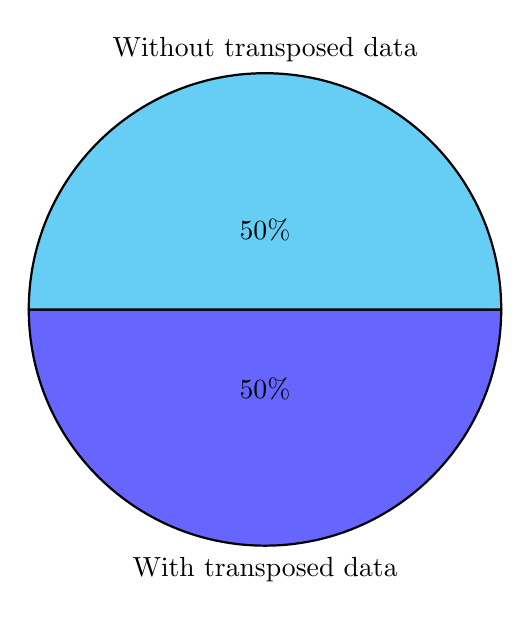
\begin{tikzpicture}
        \pie[rotate=180]{
        50/With transposed data,
        50/Without transposed data
        }
    \end{tikzpicture}
    \caption{\href{https://docs.google.com/forms/d/e/1FAIpQLSe3LEiDZFI9Y58OgWvHwKke4k1_2yPg8eJLQFBasSKUAdh3Ng/viewform?usp=sf_link}{Google Form} result on transposed data}
    The preferred model by the people
    \label{fig:pie:transpose}
    \end{center}
\end{figure}

14 people answered the it.
And the results match the expectations from the plots of the metrics.
People didn't prefer a model to another.

\section{Model size}
\label{sec:exp:size}

I tried to modify the model size to check if a bigger or smaller model could converge better.
I tried several combinations with some Grid-Search algorithm, Bayesian-Search algorithm (see appendix \ref{appendix:hp-tuning}) and by manual tries.

% The figures \ref{fig:loss-comparison-size}, \ref{fig:kld-comparison-size}, \ref{fig:loss-output-comparison-size} and \ref{fig:acc-output-comparison-size} shows respectively the value of the global loss, the KLD, the loss of one output, the accuracy of one output through 50 epochs of training for different size of models.
There are 3 size of models:
\begin{itemize}
    \item \textit{Small}: with a size of about $3000Mib$ on GPU
    \item \textit{Medium}: with a size of about $8500Mib$ on GPU
    \item \textit{Large}: with a size of about $10500Mib$ on GPU
\end{itemize}
Those memory sizes correspond to a batch size of 64.

I couldn't test with bigger model because of the GPU size limitation.

The graphs for this section are in the appendix \ref{appendix:size}.
\begin{itemize}
    \item The figure \ref{fig:loss-output-comparison-size} shows the value of the loss of an output.
    \item The figure \ref{fig:acc-output-comparison-size} shows the value of the accuracy of the loss.
    \item The figure \ref{fig:loss-comparison-size} shows the global loss value.
    \item The figure \ref{fig:kld-comparison-size} shows the KLD value.
\end{itemize}

From these different figures, we can see there is no concrete differences between the 3 models on the training data.
The values of the global loss, the accuracy and the loss for one output are basically the same.
However, the KLD value is slightly better when the model is bigger.

For the validation data, the medium model seems to perform better for every metrics.

However despite the difference of value between the different metrics, the created samples are not very different, the notes are mostly quarter notes (\musQuarter) and there is no variation is the generated music.

\begin{figure}[htbp]
    \centering
    \includegraphics[width=\textwidth]{images/experiences/size/generation-comparison-size-small.jpg}
    \caption{Pianoroll created by the small model}
    \href{https://github.com/ValentinVignal/midiGenerator/blob/master/samples/mode-size-comparison/small.mid}{Link}
    \label{fig:exp:size:generation-small}
\end{figure}

\begin{figure}[htbp]
    \centering
    \includegraphics[width=\textwidth]{images/experiences/size/generation-comparison-size-medium.jpg}
    \caption{Pianoroll created by the medium model}
    \href{https://github.com/ValentinVignal/midiGenerator/blob/master/samples/mode-size-comparison/medium.mid}{Link}
    \label{fig:exp:size:generation-medium}
\end{figure}

\begin{figure}[htbp]
    \centering
    \includegraphics[width=\textwidth]{images/experiences/size/generation-comparison-size-large.jpg}
    \caption{Pianoroll created by the large model}
    \href{https://github.com/ValentinVignal/midiGenerator/blob/master/samples/mode-size-comparison/large.mid}{Link}
    \label{fig:exp:size:generation-large}
\end{figure}

As shown in the figures \ref{fig:exp:size:generation-small}, \ref{fig:exp:size:generation-medium}, \ref{fig:exp:size:generation-large}, the created samples are quite similar through all the models.
The generated part is looping over the same notes.


I created a \href{https://docs.google.com/forms/d/e/1FAIpQLSdBn0DZZe-8YPvLYl-vovapk1iMnteeLzGfFJ7R00D3eA-Ydw/viewform?usp=sf_link}{Google Form} so people can evaluate what is the best model.
The figure \ref{fig:pie:size} displays the result of the preference of the persons who answered the survey.

\begin{figure}
    \begin{center}
    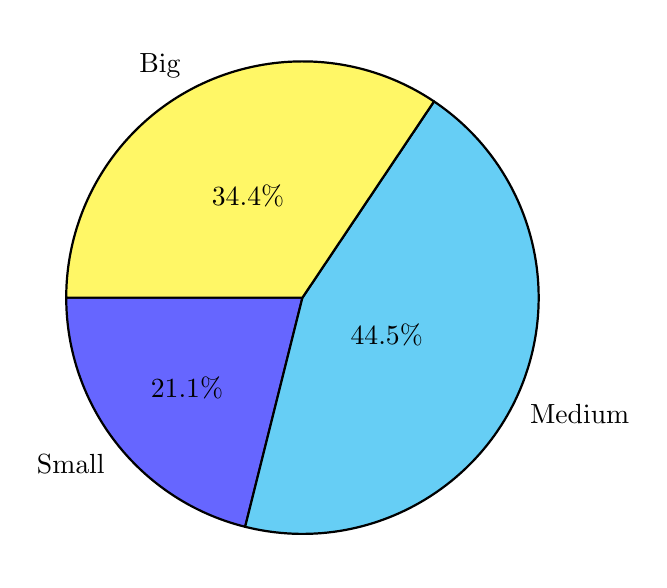
\begin{tikzpicture}
        \pie[rotate=180]{
        21.1/Small,
        44.5/Medium,
        34.4/Big
        }
    \end{tikzpicture}
    \caption{\href{https://docs.google.com/forms/d/e/1FAIpQLSdBn0DZZe-8YPvLYl-vovapk1iMnteeLzGfFJ7R00D3eA-Ydw/viewform?usp=sf_link}{Google Form} result on model size}
    The preferred model by the people
    \label{fig:pie:size}
    \end{center}
\end{figure}

32 persons answered the google form, and surprisingly, the results follow the metrics even though the generated samples are pretty similar.
This confirms that the metrics could actually be meaningful.

\section{Custom losses}

\subsection{Scale and Rhythm}
\label{sec:exp:scale-rhythm}

% with scale and rhythm : r0sr11h1b1p1
% without : r0sr00h1b1p1

The appendix \ref{appendix:scale-rhythm} contains useful graphs for this section.
The following figures display the difference of some metrics through the training of two models. The first one doesn't use the Scale and Rhythm losses while the second one uses them.
\begin{itemize}
    \item The figure \ref{fig:exp:scale-rhythm:loss-output-comparison} shows the loss of an output
    \item The figure \ref{fig:exp:scale-rhythm:acc-output-comparison} shows the accuracy of an output
    \item The figure  \ref{fig:exp:scale-rhythm:loss-comparison} shows the global loss
    \item The figure \ref{fig:exp:scale-rhythm:kld-comparison} shows the value of the KLD
    \item The figure \ref{fig:exp:scale-rhythm:harmony-comparison} shows the Harmony value. Both of the models are using the harmony loss
    \item The figure \ref{fig:exp:scale-rhythm:all-output-comparison} shows the value of the Scale and Rhythm losses.
\end{itemize}

As we can see on the figures, there is no much difference between the two models.
However, for the validation set, the model which doesn't use the scale and rhythm losses performs better than the other one for the accuracy and the loss of an output (figures \ref{fig:exp:scale-rhythm:loss-output-comparison} and \ref{fig:exp:scale-rhythm:acc-output-comparison}) and the global loss and the KLD value (figures \ref{fig:exp:scale-rhythm:loss-comparison} and \ref{fig:exp:scale-rhythm:kld-comparison}).

Both of the trained models here are using the harmony loss.
From the figure \ref{fig:exp:scale-rhythm:harmony-comparison}, we can see that both of the models have the same harmony value on the train and validation dataset.
It would mean the scale-and-rhythm losses and the harmony loss don't affect each other.

The scale and rhythm loss value in the figure \ref{fig:exp:scale-rhythm:all-output-comparison} are obviously different between the two models since the first one doesn't use those loss functions.

The figures \ref{fig:exp:scale-rhythm:with} and \ref{fig:exp:scale-rhythm:without} show respectively 2 generated samples from the model using the Scale and Rhythm losses and the model which doesn't use it.


\begin{figure}[htbp]
    \centering
    \includegraphics[width=\textwidth]{images/experiences/scale-rhythm-rnn/generated-with-scale-rhythm.jpg}
    \caption{Created sample with a model trained using the Scale and Rhythm losses}
    (\href{https://github.com/ValentinVignal/midiGenerator/blob/master/samples/scale-rhythm-comparison/generated-with-scale-rhythm.mid}{Link})
    \label{fig:exp:scale-rhythm:with}
\end{figure}
\begin{figure}[htbp]
    \centering
    \includegraphics[width=\textwidth]{images/experiences/scale-rhythm-rnn/generated-without-scale-rhythm.jpg}
    \caption{Created sample with a model trained which doesn't use the Scale and Rhythm losses}
    (\href{https://github.com/ValentinVignal/midiGenerator/blob/master/samples/scale-rhythm-comparison/generated-without-scale-rhythm.mid}{Link})
    \label{fig:exp:scale-rhythm:without}
\end{figure}

From the samples showed in the figures \ref{fig:exp:scale-rhythm:with} and \ref{fig:exp:scale-rhythm:without}, it looks like the sample from the model using the scale and rhythm losses is more complex and has more variations than the one generated by the other model.

We could think that with the help of the scale loss, the harmony value of the generated samples would show some pertinent results.
Unfortunately, it was not the case, the harmony value of the seeds given to the model was in average $0.094$,
From all the samples I have generated the harmony value for the model without the scale and rhythm loss is $0.087$ and the one using the custom loss function is $0.081$ which is slightly lower.
The figures \ref{fig:exp:scale-rhythm:harmony-generated:with} and \ref{fig:exp:scale-rhythm:harmony-generated:without} respectively show the value of the harmony value per measure of the samples showed in the figures \ref{fig:exp:scale-rhythm:with} and \ref{fig:exp:scale-rhythm:without}.




I created a \href{https://docs.google.com/forms/d/e/1FAIpQLSckCvIg1mZdXlh1fSv_yG68dEbfQRN-WwkGG2KVdcjQ4rQgbw/viewform?usp=sf_link}{Google Form} so people can evaluate what is the best model.
The figure \ref{fig:pie:scale-loss} display the result of the preference of the persons who answered to the poll.

\begin{figure}
    \begin{center}
    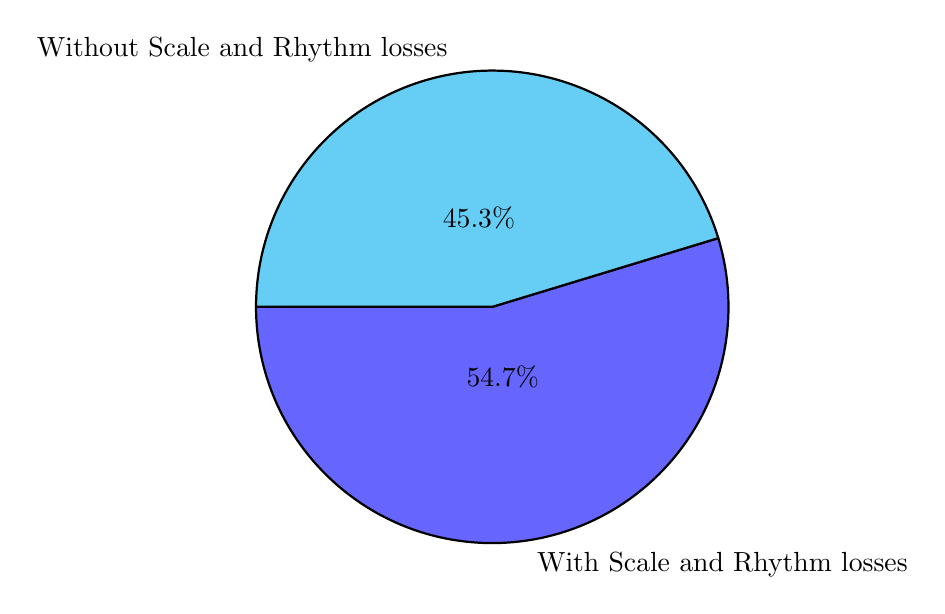
\begin{tikzpicture}
        \pie[rotate=180]{
        54.7/With Scale and Rhythm losses,
        45.3/Without Scale and Rhythm losses
        }
    \end{tikzpicture}
    \caption{\href{https://docs.google.com/forms/d/e/1FAIpQLSckCvIg1mZdXlh1fSv_yG68dEbfQRN-WwkGG2KVdcjQ4rQgbw/viewform?usp=sf_link}{Google Form} result on Scale and Rhythm losses}
    The preferred model by the people
    \label{fig:pie:scale-loss}
    \end{center}
\end{figure}

17 persons answered the google form.
And in that case, the result of the survey doesn't match the metrics but match my feeling about the generated samples.
People slightly preferred the samples created by the model with the scale and rhythm losses.



\subsection{Harmony}
\label{sec:exp:harmony}

% With: r0sr00h1b1p1
% Without: r0sr00h0b1p1

The appendix \ref{appendix:harmony} contains useful graphs for this section.
The following figures display the differences for some metrics through the training of two models.
The first one uses the custom loss \textit{Harmony}, and the second one doesn't use it.
\begin{itemize}
    \item The figure \ref{fig:acc-output-comparison-harmony} shows the accuracy of an output
    \item The figure \ref{fig:loss-output-comparison-harmony} shows the loss of an output
    \item The figure \ref{fig:loss-comparison-harmony} shows the global loss
    \item The figure \ref{fig:harmony-comparison-harmony} shows the harmony loss value
    \item The figure \ref{fig:kld-comparison-harmony} shows the KLD value
\end{itemize}


As we can see in the figure \ref{fig:acc-output-comparison-harmony}, there is no difference between the two models, the accuracy of an output is basically the same.
The same ascertainment can be done with the loss of an output (figure \ref{fig:loss-output-comparison-harmony}), the values are pretty similar.

However, the value of the loss function (figure \ref{fig:loss-comparison-harmony}) of the model which uses the Harmony loss is higher.
It can been explain because the second model doesn't use the harmony loss (see figure \ref{fig:harmony-comparison-harmony}), therefore the harmony loss value is not added to the global loss.

Because of time issues, I couldn't train the model using the Harmony loss too long.
So I trained the first model for 20 epochs and the second one for 50 epochs.
This is why the KLD value \ref{fig:kld-comparison-harmony} between the models is different.
Therefore the $\beta$ annealing (appendix \ref{appendix:kld-annealing}) follows a different evolution.
What we can notice, it that the final value of the KLD is basically the same for the validation set and the training set.


The figures \ref{fig:exp:harmony:with} and \ref{fig:exp:harmony:without} show respectively 2 generated samples from the model using the Harmony loss and the model which doesn't use it.

\begin{figure}[htbp]
    \centering
    \includegraphics[width=\textwidth]{images/experiences/harmony-rnn/with-harmony.jpg}
    \caption{Created sample with a model trained using the Harmony Loss}
    (\href{https://github.com/ValentinVignal/midiGenerator/blob/master/samples/harmony-comparison/generated_with_harmony.mid}{Link})
    \label{fig:exp:harmony:with}
\end{figure}
\begin{figure}[htbp]
    \centering
    \includegraphics[width=\textwidth]{images/experiences/harmony-rnn/without-harmony.jpg}
    \caption{Created sample with a model trained which doesn't use the Harmony loss}
    (\href{https://github.com/ValentinVignal/midiGenerator/blob/master/samples/harmony-comparison/generated_without_harmony.mid}{Link})
    \label{fig:exp:harmony:without}
\end{figure}

From these samples, it is not obvious to determine whether the loss is helping the model or not.
Maybe the produced samples from the model using the Harmony loss are \textit{"smoother"} than the other one, but this is very subtle.

The harmony value of the samples created by the different model are in average $0.092$ for the one not using the harmony loss and $0.087$ for the one using it.
The average of the harmony value in the seeds is $0.095$.
As expected the value of the harmony loss is lower for the model using the custom loss function.
The figures \ref{fig:exp:harmony:generated-harmony:with} and \ref{fig:exp:harmony:generated-harmony:without} respectively show the harmony value per measure of the samples showed in the figures \ref{fig:exp:harmony:with} and \ref{fig:exp:harmony:without}.

I created a \href{https://docs.google.com/forms/d/e/1FAIpQLScZ1ZAkCxwIRiuewNlDUFgZcpEY2O-Yg0T8IEQzp4k9_BCCJg/viewform?usp=sf_link}{Google Form} so people can evaluate what is the best model.
The figure \ref{fig:pie:harmony} displays the result of the preference of the persons who completed the survey.

\begin{figure}
    \begin{center}
    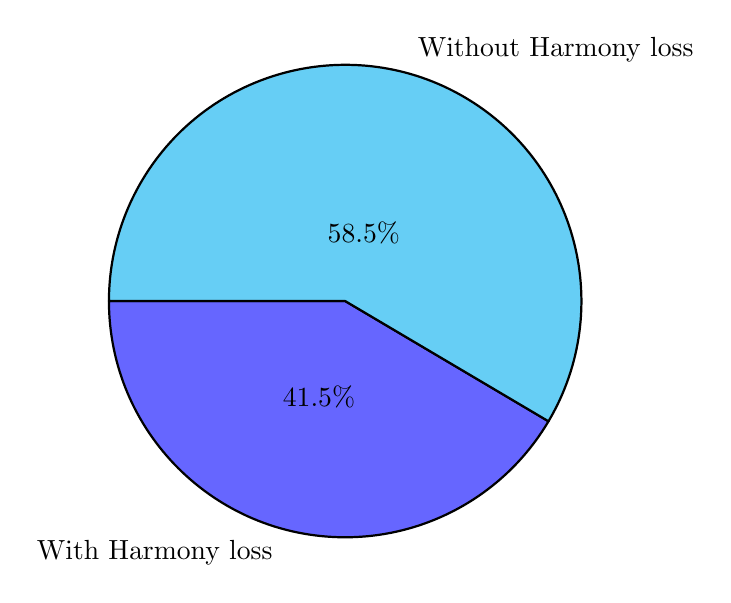
\begin{tikzpicture}
        \pie[rotate=180]{
        41.5/With Harmony loss,
        58.5/Without Harmony loss
        }
    \end{tikzpicture}
    \caption{\href{https://docs.google.com/forms/d/e/1FAIpQLScZ1ZAkCxwIRiuewNlDUFgZcpEY2O-Yg0T8IEQzp4k9_BCCJg/viewform?usp=sf_link}{Google Form} result on Harmony loss}
    The preferred model by the people
    \label{fig:pie:harmony}
    \end{center}
\end{figure}

22 persons answered the google form.
Unfortunately, the people have preferred the model which doesn't use the harmony loss.
It is quite disappointing and I was hoping the harmony loss would have helped the model.


\section{RPoE}
\label{sec:exp:rpoe}

The appendix \ref{appendix:exp:rpoe} contains useful figures for this section.
The following figures display the differences of the value of the several metrics during the training of two models.
The first model doesn't use a RPoE layer, and the second model is using it.
\begin{itemize}
    \item The figure \ref{fig:acc-output-comparison-rpoe} shows the accuracy of one output
    \item The figure \ref{fig:loss-output-comparison-rpoe} shows the loss of on output
    \item The figure \ref{fig:loss-comparison-rpoe} shows the global loss value
    \item The figure \ref{fig:kld-comparison-rpoe} shows the KLD value
    \item The figure \ref{fig:harmony-comparison-rpoe} shows the harmony loss value
    \item The figure \ref{fig:all-output-comparison-rpoe} shows the scale and rhythm losses value
\end{itemize}

As we can see on the figures \ref{fig:acc-output-comparison-rpoe}, \ref{fig:loss-output-comparison-rpoe}, \ref{fig:harmony-comparison-rpoe}, the accuracy and loss values of an output are not different between the two models for the training and validation set.

On the figure \ref{fig:all-output-comparison-rpoe}, it appears that on the validation set, the value of the scale and rhythm losses and seems to be better for the model which doesn't use the RPoE layer.

Finally, on the figures \ref{fig:loss-comparison-rpoe} and \ref{fig:kld-comparison-rpoe}, it appears the value of the KLD of the model using the RPoE is 2 times bigger than the one which doesn't use the RPoE.

From these results, it seems that the model using a RPoE layer doesn't perform better than the model that doesn't use the RPoE layer.

However, the samples sound a bit better to me when they are produced by the model containing a RPoE layer.
In my opinion, there are more variations and the repeated sequence is more complex.
The figures \ref{fig:exp:rpoe:with} and \ref{fig:exp:rpoe:without} show 2 generated samples.
The first one comes from the model with the RPoE layer and the second one comes from the model without the RPoE layer.

\begin{figure}[htbp]
    \centering
    \includegraphics[width=\textwidth]{images/experiences/rpoe-rnn/generated-with-rpoe.jpg}
    \caption{Created sample with a model trained using the RPoE layer}
    (\href{https://github.com/ValentinVignal/midiGenerator/blob/master/samples/rpoe-comparison/generated-with-rpoe.mid}{Link})
    \label{fig:exp:rpoe:with}
\end{figure}
\begin{figure}[htbp]
    \centering
    \includegraphics[width=\textwidth]{images/experiences/rpoe-rnn/generated-without-rpoe.jpg}
    \caption{Created sample with a model trained which doesn't use the RPoE layer}
    (\href{https://github.com/ValentinVignal/midiGenerator/blob/master/samples/rpoe-comparison/generated-without-rpoe.mid}{Link})
    \label{fig:exp:rpoe:without}
\end{figure}

I created a \href{https://docs.google.com/forms/d/e/1FAIpQLSf1tkCLj78u-IoMYjGWa3iTYWIT_gbPnGIShjFox4whfhkjLw/viewform?usp=sf_link}{Google Form} so people can evaluate what is the best model.
The figure \ref{fig:pie:rpoe} displays the result of the preference of the persons who completed the survey.


\begin{figure}
    \begin{center}
    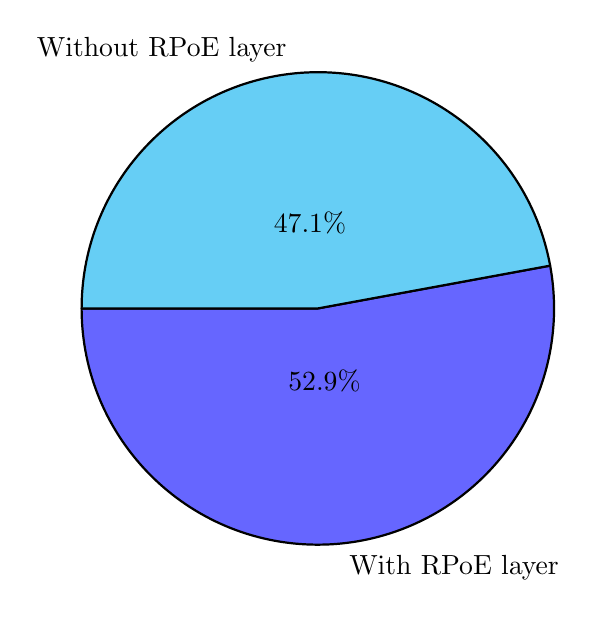
\begin{tikzpicture}
        \pie[rotate=180]{
        52.9/With RPoE layer,
        47.1/Without RPoE layer
        }
    \end{tikzpicture}
    \caption{\href{https://docs.google.com/forms/d/e/1FAIpQLSf1tkCLj78u-IoMYjGWa3iTYWIT_gbPnGIShjFox4whfhkjLw/viewform?usp=sf_link}{Google Form} result on PRoE layer}
    The preferred model by the people
    \label{fig:pie:rpoe}
    \end{center}
\end{figure}

14 persons answered the google form.
In that case the results of the survey match the suppositions from the metrics.
Using a RPoE layer doesn't add anything to the generation.



% ----------------------------------------------------------------------------------------------------
% Conclusion
% ----------------------------------------------------------------------------------------------------

\chapter{Conclusion}

The objective of my dissertation was to create a unique model to perform several tasks a musician could do as create a song, arrange one, create an accompaniment from a melody or create a melody from an accompaniment... 
However, the current works done about music generation using deep learning solution mostly focus on one objective.

In this work, I have created a new architecture called \textbf{RMVAE} (Recurrent Multimodal Variational AutoEncoder).
This architecture allows me to train only one model to perform several music generation tasks as:
\begin{itemize}
    \item Generating or completing one or several musical parts
    \item Creating one or several musical part(s) from one or several musical part(s).
    Each of them could be an accompaniment or a melody part
    \item Redoing a song by iteratively change a musical part after another
\end{itemize}
Moreover, the agile architecture and implementation of the \textbf{RMVAE} easily allows us to implement other tasks like reconstructing a missing measure, only consider some specific parts to generate others...
I created a new neural network layer called RPoE (Recurrent Product of Expert).
And finally, I came up with 3 additional loss functions to give prior knowledge to the model.
These loss functions are based on my understanding of music and on some physical phenomena as the musical harmonics and the resonance phenomena.

However, even though the \textbf{RMVAE} is general and can perform many tasks, the results are far from my expectations.
While DeepBach \cite{hadjeres_deepbach:_2016} or BachBot \cite{liang_automatic_2017} create realistic Bach's style music, my model gets stuck and usually produces the same sequence over and over.
The looping sequence is usually mostly composed of Quarter notes (\musQuarter) and each musical parts use around 3 or 4 different notes.

I have conducted some experiments and created several surveys to allow the population to evaluate the contribution from the custom losses.
Unfortunately, the results showed that a model using a custom loss were equivalent or worse than a model that doesn't use it.

% ----------------------------------------------------------------------------------------------------
% Future work
% ----------------------------------------------------------------------------------------------------

\section*{Future work}

I believe that this approach can lead to a well trained model able to generalize music and handle most of the tasks someone could ask to a neural network.

It looks like the text encoding (section \ref{sec:rw:midi:text}) is the one which performs the best for Bach's style music generation \cite{hadjeres_deepbach:_2016, liang_automatic_2017}.
This is something I can't explain because letters and words structure is, in my opinion, not linked in any way to musical notes structure.
Even though I don't understand it, this would be a possible solution to improve the model's performance.

The \textit{Scale} and \textit{Rhythm} loss functions could be ameliorated.
A scale template could be created to fit the local scale.
This template could contain some weights related the importance of the notes.
A \textit{strong} weight would give a \textit{strong} reward to the produced notes.
Those weights would be decreasing following the harmonics order (Tonic, Fifth, Major Third...) or the Third cycle (Tonic, Major Third, Fifth...) to fit music and chords theory.
This would encourage the model to produce notes that are not already in the target tensor but will (hopefully) still be musically correct.

If a dataset contains some additional information about music (like chords, local scale...), it would allow us integrate a deeper prior knowledge to the neural network.

The slowness of deep learning training, the leak memory issues, and the limited resources have been the biggest constraints for my Dissertation.
A deep and large investigation about all the different hyper-parameters used in my project, using for instance a Grid-Search or a Bayesian-Search algorithm, would dramatically help to trained a powerful \textbf{RMVAE}.


\newpage

% ####################################################################################################
% ####################################################################################################
% Bibliography
% ####################################################################################################
% ####################################################################################################
\bibliographystyle{IEEEtran}
\bibliography{IEEEabrv, biblio/Dissertation.bib}
% \printbibliography

% ####################################################################################################
% ####################################################################################################
% Appendix
% ####################################################################################################
% ####################################################################################################

\newpage

\chapter*{Appendices}
\addcontentsline{toc}{chapter}{Appendices}      % To not display number of chapter in table of content
\appendix

\section{Interpolation project}

At the start of my Dissertation, I first tried another project which was to create music with a waveform representation.
Subham S. Sahoo et al. \cite{sahoo_learning_2018} present their improved network for equation learning $\text{EQL}^\div$, that overcomes the limitation of the earlier works. In particular, their main contribution are:
\begin{itemize}
    \item They propose a network architecture that can handle divisions as well as techniques to keep training stable
    \item They improve model/instance selection to be more effective in identifying the right network/equation
    \item They demonstrate how to reliably control a dynamical robotic system by learning its forward dynamics equations from very few random tryouts/tails.
\end{itemize}

More precisely, their model is a shallow network able to learn complex function containing multiplication, sine and cosine functions, and it is able to extrapolate them.
Those are very usual operations processed by most of the VST to create musical sounds.

Thereby, I tried to interpolate musical waveform with their architecture.
My idea was to construct a transition between 2 parts (for example a verse and a chorus) or reconstruct some missing data from a song.

Unfortunately, the results were poor...
Most of the time, the model was converging to the mean of the functions (which is 0 for musical waveform).

I think their model is working well for their applications because they use it to extrapolate robotic dynamic equations which usually don't include many sine and cosine components.
Contrariwise, a musical waveform contains an enormous number of sine and cosine components. 


\section{Segment Sum}
\label{appendix:segment_sum}

The segment sum operation allows me to sum the values of a vector of shape \texttt{(128,)} (corresponding of all the different notes in the different octaves) in a vector of shape \texttt{(12,)} (corresponding to the different 12 notes).

The figure \ref{fig:segment_sum} describes what the segment sum operation would perform if there were only 4 different notes (\textit{A, B, C, D}) and 3 different octaves (\textit{1, 2, 3}) for a total of 12 notes.

\begin{figure}[ht]
    \centering
    \includegraphics[width=\textwidth]{images/nn/tensor/segment_sum.jpg}
    \caption{Segment sum operation}
    \label{fig:segment_sum}
\end{figure}

\section{$\text{Roll}_n$}
\label{appendix:roll_n}

The $\text{Roll}_n$ operation takes a one dimensional tensor, takes the first $n$ values and put them at the end.
The algorithm \ref{alg:roll_n} explains how it works and the figure \ref{fig:roll_2} shows an example with $n=2$.

\begin{algorithm}
    \begin{algorithmic}[1]
        \Require{tensor, n} 
        \Ensure{$tensor$ (Rolled tensor)}
        \Statex
        \Function{Roll}{$tensor, n$}
            \For{$k \gets 1$ to $n$}
                \State {$firstElement \gets tensor.pop(0)$}
                \State {$tensor.append(firstElement)$}
            \EndFor
            \State \Return {$tensor$}
        \EndFunction
        \end{algorithmic}
    \caption{$\text{Roll}_n$ function}
    \label{alg:roll_n}
\end{algorithm}

\begin{figure}[ht]
    \centering
    \includegraphics[width=\textwidth]{images/nn/tensor/roll_2.jpg}
    \caption{$\text{Roll}_2$ example}
    \label{fig:roll_2}
\end{figure}

\section{BandPlayer}

Training a model and generating music is interesting.
But as musician, I wasn't fully satisfied with this application.
To fulfil my needs, I created a python script to be able to play with the trained model in real time.
I call this application \texttt{BandPlayer} because the user can play with and jam with a virtual band.

The application I have created
\begin{itemize}
    \item Allows the user to play music with the instrument of his choice
    \item Can load a trained model
    \item Allows the user to choose what part he wants to play in the \textit{"band"}
    \item Allows the user to choose what parts from the \textit{"band"} he wants to play with
    \item Feeds the model with the notes played 
    \item Play the produced notes by the model with the user
    \item Display the notes played by the model and the user in a pianoroll view
\end{itemize}

Calling the model to make the notes prediction while the user is playing is computationally feasible because my model is working on an entire measure at one time.
Therefore, the model is called only one time per measure which is not to frequent to allow the application to be real time.


\section{Coconet Process}
\label{appendix:coconet_process}

The figure \ref{fig:coconet_process} illustrates the coconet process.
This process is explained in the section \ref{sec:rw:nade}.

\begin{figure}[htbp]
    \centering
    \includegraphics[width=0.8\textwidth]{images/related_works/coconet/coconet_process.jpg}
    \caption{COCONET process}
    Source: Cheng-Zhi Anna Huang et al.'s paper \cite{huang_counterpoint_2017}
    \label{fig:coconet_process}
\end{figure}

\section{Transformer architecture}

The figure \ref{fig:arch:transformer} illustrates the transformer's architecture. This architecture is explained in the section \ref{sec:back:transformers}.

\begin{figure}[htbp]
    \centering
    \includegraphics[width=\textwidth]{images/related_works/transformer/transformer_architecture.jpg}
    \caption{Transformer architecture}
    Source: Ashish Vaswani et al.'s paper \cite{vaswani_attention_2017-1}
    \label{fig:arch:transformer}
\end{figure}

\section{Hyper-Parameters tuning}
\label{appendix:hp-tuning}

Tuning hyper-parameters to train the best possible model is a difficult task in deep learning.
The reason is because every number or setting can be considered as a hyper-parameter and, most of time, there is no proof or rules to guide us to choose the best value a parameter should have.
The only help a researcher can have is his intuition and his understanding on how a specific parameter will influence a specific process.

A common doing is to implement a grid-search algorithm.
For each hyper-parameters, a set of possible value is specified and the algorithm is simply to train the model with all the possible combinations of parameters.
However, the number of iterations grows exponentially with the number of hyper-parameters.

It has been showed that a random-search algorithm is in average faster and better than a grid search.

Another possibility is to implement a Bayesian optimization \cite{frazier_tutorial_2018, adams_tutorial_nodate}.
It is a sequential design strategy for global optimization of black-box functions that doesn't require derivatives.
It uses GP to learn a unknown function.
Since the number of hyper-parameters in my project is very high, (at some point, I was trying to tune over 20 parameters), I implemented a script to do a Bayesian Search over them.
To do so I used the library scikit-optimize \cite{noauthor_scikit-optimize_nodate}.
The main advantages of a Bayesian Search over a Grid or a Random Search are:
\begin{itemize}
    \item It requires less iterations.
    \item The domain of search for a specific parameter value is not discrete but continuous.
\end{itemize}


\section{Implementation details}

My project is coded in Python language.
I have made my GitHub repository accessible at \url{https://github.com/ValentinVignal/midiGenerator}.

\subsection{Network details}

To create and train my models I used the python frameworks Tensorflow \cite{noauthor_tensorflow_nodate} and Keras \cite{noauthor_keras_nodate}.

\subsubsection{Hyper Parameters}

The table \ref{tab:network-hp} lists the value of the principal hyper-parameters used.

\begin{table}[htbp]
    \centering
    \begin{tabular}{c|c}
        Hyper Parameter & Value \\
        \hline
        optimizer &  Adam optimizer \cite{brownlee_gentle_2017, bushaev_adam_2018, kingma_adam_2017} \\
        learning rate & $10^{-3}$ \\
        fully connected layer dropout & $10^{-2}$ \\
        convolutional layer dropout & $10^{-3}$ \\
        lstm dropout & $10^{-3}$ \\
        decay & $10^{-1}$ \\
        $\lambda_{\text{scale}}$ & $10^{-1}$ \\
        $\lambda_{\text{rhythm}}$ & $10^{-2}$ \\
        $\lambda_{\text{semitone}}$ & $10^{-2}$ \\
        $\lambda_{\text{tone}}$ & $10^{-2}$ \\
        $\lambda_{\text{tritone}}$ & $10^{-2}$ \\
        $\text{epoch}_{\text{kld start}}$ & $10^{-2}$ \\
        $\text{epoch}_{\text{kld stop}}$ & $0.4$ \\
    \end{tabular}
    \caption{Neural Network Hyper-Parameters}
    \label{tab:network-hp}
\end{table}

Through all the manual training I manually launched, the Grid Search and Bayesian Search algorithm I ran, I have continuously been updated the value of these hyper-parameters.

\subsubsection{Masking}

To handle missing data, modalities (instruments), the model takes as input a mask.
The shape of a mask is \texttt{(nb\_instruments, nb\_measures)} and composed of 0 and 1.
If there is a 0 at the position $(i, m)$ of the mask, it means that the measure $m$ of the instrument $i$ is missing and the model will ignore it.


\subsection{Training details}

\subsubsection{Noise}

During the training, I insert some noise in the input data.
For monophonic music, an activation value will be changed (from 0 to 1 or from 1 to 0) with a probability $p$.
I usually have put $p \in [10^{-4}, 10^{-3}]$.
The chosen range of $p$ seems low but a higher noise can sometimes alter the input too much, even for a human ear.

For example, let's assume a noise with $p = 10^{-2}$.
A shape of a tensor representing a measure is \texttt{(16, 128)}.
For every frame (shape of \texttt{(128,)}), the expectation of altered note is $1.28$.
It is an added or deleted note for every frame (Sixteenth \musSixteenth) which completely deform the music.

\subsubsection{Tensor size}

For simplicity, I have written in all my dissertation that the shape of a tensor representing a measure was \texttt{(16, 128, channels)}.
However, because I have been sharing a GPU from NUS with other students, I tried to reduce the size of my models.
To do so, decided to reduce the pitch dimension (\texttt{(128,)}).
Instead of considering all the possible MIDI notes, I consider the minimum range of notes which contains all the notes actually present in the dataset.
This allows me to reduced the size from \texttt{128} to \texttt{58} (the range of the MIDI notes is $[\texttt{10}, \texttt{68})$).


\subsubsection{KLD Annealing}
\label{appendix:kld-annealing}

It is usually difficult to train a VAE because of the KLD which adds a substantial constraint on the latent space.
To help the model to converge, I implemented a \textit{KLD annealing} \cite{huang_improving_2018}.

\begin{equation}
    loss = loss_{output} + \beta \mathbb{D}_{KL}
\end{equation}

I linearly increases $\beta$ from 0 to 1 through the epochs from $\text{epoch}_{\text{kld start}}$ to $\text{epoch}_{\text{kld stop}}$.
Before $\text{epoch}_{\text{kld start}}$ $\beta = 0$, and after $\text{epoch}_{\text{kld stop}}$, $\beta = 1$.
For my project, I have set $\text{epoch}_{\text{kld start}} = 10^{-2}$ and $\text{epoch}_{\text{kld stop}} = 0.4$.

The equation \ref{eq:kld-annealing} and the figure \ref{fig:beta-annealing} show the evolution of $\beta$ through the training.

\begin{equation}
    \beta (\text{epoch}) =
    \begin{cases}
        0 & \text{if } \frac{\text{epoch}}{\text{epoch}_{\text{total}}} \leq \text{epoch}_{\text{kld start}} \\
        
        \frac{(\text{epoch} / \text{epoch}_{\text{total}}) - \text{epoch}_{\text{kld start}}}{\text{epoch}_{\text{kld stop}} - \text{epoch}_{\text{kld start}}} & \text{if } \text{epoch}_{\text{kld start}} \leq \frac{\text{epoch}}{\text{epoch}_{\text{total}}} \leq \text{epoch}_{\text{kld stop}} \\
        
        1 & \text{if } \frac{\text{epoch}}{\text{epoch}_{\text{total}}} \geq \text{epoch}_{\text{kld stop}} \\
    \end{cases}
    \label{eq:kld-annealing}
\end{equation}

\begin{figure}[htbp]
    \centering
    \includegraphics[width=0.8 \textwidth]{images/nn/training/beta-annealing.jpg}
    \caption{$\beta$ value through training for KLD annealing}
    \label{fig:beta-annealing}
\end{figure}

\subsubsection{Sub-sample Training Paradigm}

As explained in Mike Wu's paper for the MVAE \cite{wu_multimodal_2018}, a specific training paradigm is used to fully train the different experts.

Given a complete dataset with no missing modalities (i.e. missing instruments in my work), optimizing the equation \ref{eq:vae:elbo} is not optimal: the individual inference networks are never trained and thus, the model does not know how to use them when it encounters any missing data at test time.
Conversely, if the model is trained only on independent modalities, it will fail to capture the relationship between modalities in the generative model.
The idea is to combine the two extremes, including ELBO terms for whole and partial observations.
However, if there are $N$ modalities, training on every possible subsets would be computationally intractable (there are $2^{N}$ subsets).
To reduce the cost, the ELBO terms to optimize are sub-sampled.
Specifically, they chosen ones are (1) the ELBO using the product of $N$ Gaussians, (2) all ELBO terms using a single modality, and (3) $k$ ELBO terms using $k$ randomly chosen subsets $X_k$.
For each minibatch, I evaluate a random subset of the $2^{N}$ ELBO terms.
In expectation, it approximates the full objective.

The sub-sampled objective can be written as in the equation \ref{eq:appendix:sub-sampled-elbo}.

\begin{equation}
    ELBO(x_1, \dots, x_M) + \sum_{i=1}^{N} ELBO(x_i) + \sum_{j=1}^{k} ELBO(X_j)
    \label{eq:appendix:sub-sampled-elbo}
\end{equation}

In practice, $k = 2$

\section{Google Forms}
\label{appendix:google-forms}


For this Dissertation I created several google forms to determine what model was better than the other.
Here are the links of all the google forms I have created:
\begin{itemize}
    \item For the tranposed data (section \ref{sec:exp:transpose}): \href{https://docs.google.com/forms/d/e/1FAIpQLSe3LEiDZFI9Y58OgWvHwKke4k1_2yPg8eJLQFBasSKUAdh3Ng/viewform?usp=sf_link}{Google Form Link}
    \item For the size of the model (section \ref{sec:exp:size}):  \href{https://forms.gle/BdEcYZgYWXPigSdA6}{Google Form link}
    \item For scale and rhythm loss (section \ref{sec:exp:scale-rhythm}): \href{https://docs.google.com/forms/d/e/1FAIpQLSckCvIg1mZdXlh1fSv_yG68dEbfQRN-WwkGG2KVdcjQ4rQgbw/viewform?usp=sf_link}{Google Form link}
    \item For the harmony loss (section \ref{sec:exp:harmony}): \href{https://docs.google.com/forms/d/e/1FAIpQLScZ1ZAkCxwIRiuewNlDUFgZcpEY2O-Yg0T8IEQzp4k9_BCCJg/viewform?usp=sf_link}{Google From link}
    \item For the RPoE layer (section \ref{sec:exp:rpoe}): \href{https://docs.google.com/forms/d/e/1FAIpQLSf1tkCLj78u-IoMYjGWa3iTYWIT_gbPnGIShjFox4whfhkjLw/viewform?usp=sf_link}{Google Form Link}
\end{itemize}

\section{Experiment plots}
\label{appendix:exp}

This section contains the plots of the different experiments from the chapter \ref{chap:experiments}.

\subsection{Transposed data}
\label{appendix:transpose}

This section contains the graphs from the section \ref{sec:exp:transpose} (figures \ref{fig:loss-output-comparison-transpose}, \ref{fig:acc-output-comparison-transpose}, \ref{fig:loss-comparison-transpose}, \ref{fig:kld-comparison-transpose}, \ref{fig:harmony-comparison-transpose}, \ref{fig:all-outputs-comparison-transpose}).

\begin{figure}[htbp]
    \begin{minipage}{0.5\textwidth}
        \begin{center}
            \includegraphics[width=\textwidth]{images/experiences/transpose-rnn/loss-output-comparison-transpose.jpg}
            \caption{Loss value of an output for models training on transposed and non transposed data}
            \label{fig:loss-output-comparison-transpose}
        \end{center}
    \end{minipage} \hfill
    \begin{minipage}{0.5 \textwidth}
        \begin{center}
            \includegraphics[width=\textwidth]{images/experiences/transpose-rnn/acc-output-comparison-transpose.jpg}
            \caption{Accuracy value for an output for models training on transposed data and non transposed data}
            \label{fig:acc-output-comparison-transpose}
        \end{center}
    \end{minipage}
\end{figure}

\begin{figure}[htbp]
    \begin{minipage}{0.5\textwidth}
        \begin{center}
            \includegraphics[width=\textwidth]{images/experiences/transpose-rnn/loss-comparison-transpose.jpg}
            \caption{Global loss for models training on transposed and non transposed data}
            \label{fig:loss-comparison-transpose}
        \end{center}
    \end{minipage} \hfill
    \begin{minipage}{0.5 \textwidth}
        \begin{center}
            \includegraphics[width=\textwidth]{images/experiences/transpose-rnn/kld-comparison-transpose.jpg}
            \caption{KLD value for models training on transposed data and non transposed data}
            \label{fig:kld-comparison-transpose}
        \end{center}
    \end{minipage}
\end{figure}

\begin{figure}[htbp]
    \begin{minipage}{0.5\textwidth}
        \begin{center}
            \includegraphics[width=\textwidth]{images/experiences/transpose-rnn/harmony-comparison-transpose.jpg}
            \caption{Harmony loss for models training on transposed and non transposed data}
            \label{fig:harmony-comparison-transpose}
        \end{center}
    \end{minipage} \hfill
    \begin{minipage}{0.5 \textwidth}
        \begin{center}
            \includegraphics[width=\textwidth]{images/experiences/transpose-rnn/all-outputs-comparison-transpose.jpg}
            \caption{Scale and Rhythm loss value for models training on transposed data and non transposed data}
            \label{fig:all-outputs-comparison-transpose}
        \end{center}
    \end{minipage}
\end{figure}

\subsection{Model size}
\label{appendix:size}

This section contains the graphs from the section \ref{sec:exp:size} (figures \ref{fig:loss-output-comparison-size}, \ref{fig:acc-output-comparison-size}, \ref{fig:loss-comparison-size}, \ref{fig:kld-comparison-size}).

\begin{figure}[htbp]
    \begin{minipage}{0.5\textwidth}
        \begin{center}
            \includegraphics[width=\textwidth]{images/experiences/size/loss-output-comparison-size.jpg}
            \caption{Loss of one voice for different size of models}
            \label{fig:loss-output-comparison-size}
        \end{center}
    \end{minipage} \hfill
    \begin{minipage}{0.5 \textwidth}
        \begin{center}
            \includegraphics[width=\textwidth]{images/experiences/size/acc-output-comparison-size.jpg}
            \caption{Loss of one voice for different size of models}
            \label{fig:acc-output-comparison-size}
        \end{center}
    \end{minipage}
\end{figure}

\begin{figure}[htbp]
    \begin{minipage}{0.5\textwidth}
        \begin{center}
            \includegraphics[width=\textwidth]{images/experiences/size/loss-comparison-size.jpg}
            \caption{Global loss for different size of models}
            \label{fig:loss-comparison-size}
        \end{center}
    \end{minipage} \hfill
    \begin{minipage}{0.5 \textwidth}
        \begin{center}
            \includegraphics[width=\textwidth]{images/experiences/size/kld-comparison-size.jpg}
            \caption{KLD value for different size of models}
            \label{fig:kld-comparison-size}
        \end{center}
    \end{minipage}
\end{figure}


\subsection{Scale and Rhythm}
\label{appendix:scale-rhythm}

This section contains the graphs from the section \ref{sec:exp:scale-rhythm} (figures \ref{fig:exp:scale-rhythm:loss-output-comparison}, \ref{fig:exp:scale-rhythm:acc-output-comparison}, \ref{fig:exp:scale-rhythm:loss-comparison}, \ref{fig:exp:scale-rhythm:kld-comparison}, \ref{fig:exp:scale-rhythm:harmony-comparison},
\ref{fig:exp:scale-rhythm:all-output-comparison}).
The figures \ref{fig:exp:scale-rhythm:harmony-generated:with} and \ref{fig:exp:scale-rhythm:harmony-generated:without} respectively show the harmony value per measure for the created samples from the figures \ref{fig:exp:scale-rhythm:with} and \ref{fig:exp:scale-rhythm:without}.

\begin{figure}[htbp]
    \begin{minipage}{0.5\textwidth}
        \begin{center}
            \includegraphics[width=\textwidth]{images/experiences/scale-rhythm-rnn/loss-output-comparison-scale-rhythm.jpg}
            \caption{Loss value for one output comparison with and without scale and rhythm loss}
            \label{fig:exp:scale-rhythm:loss-output-comparison}
        \end{center}
    \end{minipage} \hfill
    \begin{minipage}{0.5 \textwidth}
        \begin{center}
            \includegraphics[width=\textwidth]{images/experiences/scale-rhythm-rnn/acc-output-comparison-scale-rhythm.jpg}
            \caption{Accuracy value for one output comparison with and without scale and rhythm loss}
            \label{fig:exp:scale-rhythm:acc-output-comparison}
        \end{center}
    \end{minipage}
\end{figure}

\begin{figure}[htbp]
    \begin{minipage}{0.5\textwidth}
        \begin{center}
            \includegraphics[width=\textwidth]{images/experiences/scale-rhythm-rnn/loss-comparison-scale-rhythm.jpg}
            \caption{Loss value for one output comparison with and without scale and rhythm loss}
            \label{fig:exp:scale-rhythm:loss-comparison}
        \end{center}
    \end{minipage} \hfill
    \begin{minipage}{0.5 \textwidth}
        \begin{center}
            \includegraphics[width=\textwidth]{images/experiences/scale-rhythm-rnn/kld-comparison-scale-rhythm.jpg}
            \caption{Loss value for one output comparison with and without scale and rhythm loss}
            \label{fig:exp:scale-rhythm:kld-comparison}
        \end{center}
    \end{minipage}
\end{figure}

\begin{figure}[htbp]
    \begin{minipage}{0.5\textwidth}
        \begin{center}
            \includegraphics[width=\textwidth]{images/experiences/scale-rhythm-rnn/harmony-comparison-scale-rhythm.jpg}
            \caption{Harmony value for one output comparison with and without scale and rhythm loss}
            \label{fig:exp:scale-rhythm:harmony-comparison}
        \end{center}
    \end{minipage} \hfill
    \begin{minipage}{0.5 \textwidth}
        \begin{center}
            \includegraphics[width=\textwidth]{images/experiences/scale-rhythm-rnn/loss-all-comparison-scale-rhythm.jpg}
            \caption{Scale and Rhythm value for one output comparison with and without scale and rhythm loss}
            \label{fig:exp:scale-rhythm:all-output-comparison}
        \end{center}
    \end{minipage}
\end{figure}

\begin{figure}[htbp]
    \begin{minipage}{0.5\textwidth}
        \begin{center}
            \includegraphics[width=\textwidth]{images/experiences/scale-rhythm-rnn/generated-harmony-with-scale-rhythm.jpg}
            \caption{Harmony value for per measure for the sample generated with the model using the Scale and Rhythm loss}
            Sample of the figure \ref{fig:exp:scale-rhythm:with}
            \label{fig:exp:scale-rhythm:harmony-generated:with}
        \end{center}
    \end{minipage} \hfill
    \begin{minipage}{0.5 \textwidth}
        \begin{center}
            \includegraphics[width=\textwidth]{images/experiences/scale-rhythm-rnn/generated-harmony-without-scale-rhythm.jpg}
            \caption{Harmony value for per measure for the sample generated with the model not using the Scale and Rhythm loss}
            Sample of the figure \ref{fig:exp:scale-rhythm:without}
            \label{fig:exp:scale-rhythm:harmony-generated:without}
        \end{center}
    \end{minipage}
\end{figure}

\subsection{Harmony}
\label{appendix:harmony}

This section contains the graphs from the section \ref{sec:exp:harmony} (figures \ref{fig:acc-output-comparison-harmony}, \ref{fig:loss-output-comparison-harmony}, \ref{fig:loss-comparison-harmony}, \ref{fig:kld-comparison-harmony}, \ref{fig:harmony-comparison-harmony}).
The figures \ref{fig:exp:harmony:generated-harmony:with} and \ref{fig:exp:harmony:generated-harmony:without} respectively show the harmony value per measure of the produced samples from a model using the harmony loss and a model that doesn't use it.
The samples are the ones from the figures \ref{fig:exp:harmony:with} and \ref{fig:exp:harmony:without}.


\begin{figure}[htbp]
    \begin{minipage}{0.5\textwidth}
        \begin{center}
            \includegraphics[width=\textwidth]{images/experiences/harmony-rnn/acc-output-comparison-harmony.jpg}
            \caption{Accuracy value for one output comparison with and without harmony loss}
            \label{fig:acc-output-comparison-harmony}
        \end{center}
    \end{minipage} \hfill
    \begin{minipage}{0.5 \textwidth}
        \begin{center}
            \includegraphics[width=\textwidth]{images/experiences/harmony-rnn/loss-output-comparison-harmony.jpg}
            \caption{Loss value for one output comparison with and without harmony loss}
            \label{fig:loss-output-comparison-harmony}
        \end{center}
    \end{minipage}
\end{figure}

\begin{figure}[htbp]
    \begin{minipage}{0.5\textwidth}
        \begin{center}
            \includegraphics[width=\textwidth]{images/experiences/harmony-rnn/loss-comparison-harmony.jpg}
            \caption{Global loss value comparison with and without harmony loss}
            \label{fig:loss-comparison-harmony}
        \end{center}
    \end{minipage} \hfill
    \begin{minipage}{0.5 \textwidth}
        \begin{center}
            \includegraphics[width=\textwidth]{images/experiences/harmony-rnn/harmony-comparison-harmony.jpg}
            \caption{Harmony loss value comparison with and without harmony loss}
            \label{fig:harmony-comparison-harmony}
        \end{center}
    \end{minipage}
\end{figure}

\begin{figure}[htbp]
    \centering
    \includegraphics[width=0.5\textwidth]{images/experiences/harmony-rnn/kld-comparison-harmony.jpg}
    \caption{KLD value comparison with and without harmony loss}
    \label{fig:kld-comparison-harmony}
\end{figure}

\begin{figure}[htbp]
    \begin{minipage}{0.5\textwidth}
        \begin{center}
            \includegraphics[width=\textwidth]{images/experiences/harmony-rnn/generated-harmony-with-harmony.jpg}
            \caption{Harmony value for per measure for the sample generated with the model using the Harmony loss}
            Sample of the figure \ref{fig:exp:harmony:without}
            \label{fig:exp:harmony:generated-harmony:with}
        \end{center}
    \end{minipage} \hfill
    \begin{minipage}{0.5 \textwidth}
        \begin{center}
            \includegraphics[width=\textwidth]{images/experiences/harmony-rnn/generated-harmony-without-harmony.jpg}
            \caption{Harmony value for per measure for the sample generated with the model no using the Harmony loss}
            Sample of the figure \ref{fig:exp:harmony:without}
            \label{fig:exp:harmony:generated-harmony:without}
        \end{center}
    \end{minipage}
\end{figure}

\subsection{RPoE}
\label{appendix:exp:rpoe}

This section contains the graphs from the section \ref{sec:exp:rpoe}(figures \ref{fig:loss-output-comparison-rpoe}, \ref{fig:acc-output-comparison-rpoe}, \ref{fig:loss-comparison-rpoe}, \ref{fig:kld-comparison-rpoe}, \ref{fig:harmony-comparison-rpoe}, \ref{fig:all-output-comparison-rpoe}).


\begin{figure}[htbp]
    \begin{minipage}{0.5\textwidth}
        \begin{center}
            \includegraphics[width=\textwidth]{images/experiences/rpoe-rnn/loss-output-comparison-rpoe.jpg}
            \caption{Loss value of an output comparison with and without RPoE layer}
            \label{fig:loss-output-comparison-rpoe}
        \end{center}
    \end{minipage} \hfill
    \begin{minipage}{0.5 \textwidth}
        \begin{center}
            \includegraphics[width=\textwidth]{images/experiences/rpoe-rnn/acc-output-comparison-rpoe.jpg}
            \caption{Accuracy value of an output comparison with and without RPoE layer}
            \label{fig:acc-output-comparison-rpoe}
        \end{center}
    \end{minipage}
\end{figure}

\begin{figure}[htbp]
    \begin{minipage}{0.5\textwidth}
        \begin{center}
            \includegraphics[width=\textwidth]{images/experiences/rpoe-rnn/loss-comparison-rpoe.jpg}
            \caption{Global loss value comparison with and without RPoE layer}
            \label{fig:loss-comparison-rpoe}
        \end{center}
    \end{minipage} \hfill
    \begin{minipage}{0.5 \textwidth}
        \begin{center}
            \includegraphics[width=\textwidth]{images/experiences/rpoe-rnn/kld-comparison-rpoe.jpg}
            \caption{KLD value comparison with and without RPoE layer}
            \label{fig:kld-comparison-rpoe}
        \end{center}
    \end{minipage}
\end{figure}

\begin{figure}[htbp]
    \begin{minipage}{0.5\textwidth}
        \begin{center}
            \includegraphics[width=\textwidth]{images/experiences/rpoe-rnn/harmony-comparison-rpoe.jpg}
            \caption{Harmony value comparison with and without RPoE layer}
            \label{fig:harmony-comparison-rpoe}
        \end{center}
    \end{minipage} \hfill
    \begin{minipage}{0.5 \textwidth}
        \begin{center}
            \includegraphics[width=\textwidth]{images/experiences/rpoe-rnn/all-output-comparison-rpoe.jpg}
            \caption{Scale and Rhythm losses value comparison with and without RPoE layer}
            \label{fig:all-output-comparison-rpoe}
        \end{center}
    \end{minipage}
\end{figure}




\end{document}

% Photographs, Illustrations and Other Attachments
% [For soft-bound, paper copy for Examination/Re-examination] Photographic and other illustrations that are to be included in the bound copy of the thesis have to be securely mounted using double-faced tape. Photograph album pockets or slits in the page are not adequate. In no circumstances should ‘cellophane tape’ or a similar material be used for any purpose in a copy of the thesis. All copies of the thesis should contain original photographs. Subsidiary papers and other loose material should be bound in wherever possible. If this is not possible, an adequately guarded pocket for each material should be provided at the end of the thesis. Any such loose material (and corrigenda sheets, if not bound in) should bear the candidate’s name, initials and degree.
% Photographic and other illustrations (e.g. line drawings, maps, musical scores, etc.) which need to be uploaded in the ETD system should be inserted in the thesis in PDF format as far as possible.
